% Template for final reports and dissertations (Instituto Politécnico de Beja)
% Version 0.8.1, 2021/10/01
% Author: João Paulo Barros, joao.barros@ipbeja.pt
% Com contribuições de Henrique Água-Doce, Nuno Mourinho e Raul Carvalho.


%para texto em Português
\documentclass[PT]{ipbeja-format}
%for text in English
%\documentclass[]{ipbeja-format}



% Para preencher 

\newcommand{\ESCOLA}{Escola Superior de Tecnologia e Gestão}
%\newcommand{\ESCOLA}{Escola Superior de Educação}
%\newcommand{\ESCOLA}{Escola Superior Agrária}
%\newcommand{\ESCOLA}{Escola Superior de Saúde}


\newcommand{\CURSO}{Licenciatura em Engenharia Informática}

\newcommand{\TITULO}{Sistema de apoio à decisão para o turismo no Alentejo}
\newcommand{\SUBTITULO}{Sistema de apoio à decisão com base em \textit{Data Mining} para o turismo no Alentejo}


\newcommand{\NOMEALUNO}{Gonçalo Amaro\\Pedro Tomás\\Vítor Abreu\\}

\newcommand{\LOCAL}{Beja}


 %se for um estágio deve ser retirado o comentário da linha seguinte e indicar o orientador na entidade de acolhimento do estágio
%\newcommand{\ORIENTADORENTIDADE}{Título académico e nome do(a) orientador(a) na entidade de acolhimento, NomeDaEntidade, por exemplo "Eng. Nome Completo ou Abreviado}

\newcommand{\ORIENTADORIPBEJAA}{Doutora Isabel Brito}
% se existir segundo orientador do IPBeja, retirar o comentário da linha seguinte
%\newcommand{\ORIENTADORIPBEJAB}{Colocar o título Académico e nome do(a) segundo(a) docente orientador(a), se existente} 


%Completar e comentar um dos seguintes dois \newcommand
%\newcommand{\DECLARACAOPROJETO}{Relatório de projecto de fim de curso apresentado na\linebreak \ESCOLA{} do Instituto Politécnico de Beja}
\newcommand{\DECLARACAO}{
Relatório de Projecto Final, realizado na cadeira de Projecto Integrado, apresentado na\linebreak \ESCOLA{} do Instituto Politécnico de Beja}

% retirar comentário e preencher se existente
%\newcommand{\DEDICATORIA}{ texto a colocar}

\usepackage[]{hyperref}
\usepackage{adjustbox}
\usepackage{pdfpages}
\usepackage{minted}

\usemintedstyle{arduino}

\hypersetup{hidelinks,hypertexnames=true}

\begin{document}
\pagenumbering{roman}
\setcounter{page}{1}
\folhacapa % 2.1 das normas
\folharosto % 2.3 das normas
%%%%%%%%%%%%%%%%%%%%%%%%%%%%%%%%%%%%%%%%%%%%
\frontmatter % parte inicial

\clearpage
\chapter{Resumo}
\section*{\textit{\TITULO}\\  {\small{\textit{\SUBTITULO}}}}


\textit
Tendo em vista uma sustentável, duradora e benéfica relação entre o turismo e o património histórico-cultural há que seguir uma estratégia. Existem várias estratégias, porém a tomada na elaboração deste trabalho foi a monitorização de fluxos de visitantes. Esta monitorização pode ser realizada através de um sistema de informação como o TripAdvisor, Zoomato e Booking, que foram os escolhidos na elaboração do trabalho, o armazenamento dos dados, ou seja, o desenvolvimento de uma base de dados em SQL, o processamento de dados usando técnicas para normalizar e analizar textos, assim como a extração das "keywords" e análise de opinião que seriam mais tarde úteis na elaboração de gráficos como medida para uma fácil visualização dos resultados acerca dos resulatos obtidos, indicando muitos aspetos interessantes acerca das preferências turísticas dentro dos patrimónios.

\clearpage
\chapter{Abstract}
\section*{\textit{Decision support system for tourism in Alentejo}\\  {\small{\textit{Decision support system based on Data Mining for tourism in Alentejo}}}}

\textit
In view of a sustainable strategy, historical establishments and cultural establishments between tourism and all places, such as hotels, in addition to historical and cultural establishments, a strategy must be followed. Several strategies, however the elaboration in the elaboration of this workflow was monitoring. This monitoring can be carried out through an information system such as TripAdvisor, Zomato and Booking, which were chosen in the elaboration of the work, the storage of data, that is, a database in SQL, the processing of data using techniques to normalize and study, as well as the extraction of "key words" and opinion analysis that will later be useful in the elaboration of measures for an easy visualization of the results about the obtained results, often interesting about the relevant issues obtained within the heritages.



% Se pretender remover, comente a linha seguinte, caso contrário preencha o ficheiro agradecimentos.tex
\clearpage
\agradecimentos

O relatório de projeto final da cadeira de Projeto Integrado decorre de uma experiência que exigiu trabalho e esforço para alcançarmos os objetivos pretendidos. Como tal, agradecemos a disponibilidade, acompanhamento atento e
colaboração demonstrados pela professora Isabel Brito, agradecemos também o seu apoio, incentivo, confiança e essencialmente por nos ter guiado para uma melhor execução do trabalho.




\clearpage
\indicegeral
\clearpage
\indicedefiguras % Remover se houver menos de 5 figuras
\clearpage
\indicedetabelas % Remover se houver menos de 5 tabelas
\clearpage
\indicedelistagens % Remover se houver menos de 5 listagens

% No caso de se verificar "um número significativamente elevado de abreviaturas e siglas" deve retirar-se o
% comentário da linha seguinte e preencher o ficheiro parte-inicial/abreviaturas.tex
%\chapter{Abreviaturas e Siglas}

\begin{longtable}{p{.15\textwidth} p{.85\textwidth}} 

IPBeja & Instituto Politécnico de Beja\\
UML & Unified Modelling Language\\
... & ...

\end{longtable}


%%%%%%%%%%%%%%%%%%%%%%%%%%%%%%%%%%%%%%%%%%%%
\mainmatter  \pagestyle{ruled} % parte principal
\pagenumbering{arabic}

\chapter{Introdução}
\label{intro}

% deve substituir as duas linhas seguintes pelo texto da introdução

\section{Objectivo do trabalho}
Este trabalho tem como principal objectivo a monitorização de fluxos de visitantes para identificar boas práticas, tendo sempre foco na criação de uma benéfica, sustentável e duradoura relação entre o turismo e o património. Para essa monitorização ser realizada, será necessário desenvolver um sistema de informação que recolha, armazena, processa e comunica dados e informação sobre as visitas ao património dos turistas nacionais e estrangeiros. Para que a essa monitorização seja realizada devidamente, será necessário que sejam realizadas algumas etapas, das quais seriam:

\begin{enumerate}
    \item A recolha de dados sobre as visitas dos turistas nacionais e estrangeiros ao património cultural de Beja, destacando-se dessa mesma recolha, as atracções, hotéis e restaurantes, e tendo como origens as fontes,  \textit{"TripAdvisor"}, \textit{"Booking"}, \textit{"Zomato"}. Para que a recolha de dados fosse realizada das devidas fontes foi necessário recorrer ao conceito de \textit{webscraping};
    \item O armazenamento de dados numa base de dados SQL, para mais tarde facilitar o gestão de toda a informação para as seguintes etapas;
    \item O processamento dos dados, iniciando-se com a sua normalização e mais tarde passando á sua análise recorrendo ao \textit{sentiment analysis} e à \textit{Keyword extraction};
    \item A elaboração de gráficos usando a biblioteca  \textit{MatplotLib} e o  \textit{software PowerBI};
\end{enumerate} 

O presente relatório encontra-se organizado na seguinte forma: \hyperref[cap2]{na secção 2} descreve-se a fase de investigação; \hyperref[cap3]{na secção 3} é descrito como foi realizado o processo de \textit{webscrapping} nos \textit{websites} mencionados, assim como a estratégia pensada e dividida pelos elementos do grupo; \hyperref[cap4]{na secção 4} é explicado o processo de normalização/formatação desenvolvido; \hyperref[cap5]{na secção 5} mostramos os métodos escolhidos na extracção das \textit{keywords}; \hyperref[cap6]{na secção 6} falamos de todo o processo por detrás dos \textit{sentiment analysis}; \hyperref[cap7]{na secção 7} de como foram gerados os gráficos ao decorrer da elaboração do projecto; \hyperref[cap8]{na secção 8} de como e do porquê de termos reorganizado o projeto e também acerca da base de dados gerada; \hyperref[cap9]{na secção 9} finalmente começamos a analisar os dados obtidos e por fim, \hyperref[cap10]{na secção 10} são apresentadas as conclusões relativas à elaboração do presente trabalho. Ao auxílio da criação deste documento foram usados os relatórios de progresso criados anteriormente.

\section{Métodos utilizados}
Para a extracção dos dados ser realizada devidamente, tal como referido, foi utilizado o conceito de \textit{webscrapping}. O conceito de \textit{webscrapping} é simplesmente a recolha de dados de uma forma automatizada, no nosso caso foi utilizada a linguagem \textit{Python} juntamente com algumas bibliotecas como a \textit{"BeautifulSoup4"}. É importante também referir que durante a elaboração do trabalho algumas ideias e conceitos foram surgindo, o que colmatou com algumas possíveis dúvidas e percurso que inicialmente o grupo pensaria que iria tomar tal como a utilização dos processos \textit{ETL (extract, transform, load)}. O grupo tinha como ideia levar o conceito á risca como ideia inicial, porém, com o decorrer do trabalho foi verificado que alguns conceitos não se encaixariam da melhor forma, mais em concreto, a fase de \textit{load}. As fases de \textit{extract} e \textit{transform} encaixam-se na perfeição, já que o trabalho consiste na extração de informação de \textit{websites} (\textit{extract}) e a sua normalização/formatação (\textit{tranform}). No entanto o processo de \textit{loading} só acabaria por ser usado como um processo secundário para outro, mais concretamente para a realização dos gráficos dentro do software \textit{PowerBI} uma vez que esta ferramenta é altamente útil para a realização de gráficos usando como base grandes quantidades de informações.

\section{Descrição e motivação}
O tema deste trabalho é bastante interessante do ponto de vista turístico e mais tarde financeiro, já que a partir dele é possível analisar as opiniões dos turistas (nacionais ou estrangeiros) e baseando-se nisso, ter noção de quais pontos turísticos, hotéis ou restaurantes cativam mais a atenção do público e também estudar os pontos fortes e fracos de cada um deles. É possível também verificar se determinados locais têm tendências a manter, aumentar ou diminuir o número de turistas com o decorrer dos anos. Estes valores são bastante importantes para um país como Portugal que usa o turismo como forte fonte de rendimento, e uma vez que no presente trabalho o foco é o Alentejo, que é altamente movimentado nas épocas balneares, mais importante a análise das informações recolhidas se tornam. 

\section{Divisão de tarefas}
Uma vez que o trabalho era realizado em grupo, foi decidido previamente que existiriam etapas onde ocorreria separação de tarefas por cada elemento do grupo, como por exemplo ao realizar o \textit{webscrapping} dos \textit{websites} pretendidos. Para além das tarefas divididas entre os elementos do grupo, foi utilizado uma ferramenta para gerir as tarefas de cada elemento respectivamente, que foi o \textit{Trello}. O \textit{Trello} é tão simples como uma ferramenta de gestão de projectos, é uma plataforma versátil e pode ser usada para acompanhamento de tarefas pessoais ou para organizar projectos que envolvam equipas/grupos com maior número de pessoas. Para além do \textit{Trello} o grupo também utilizou o \textit{GitHub} como ferramenta de gestão do trabalho e repositório do mesmo, sendo a principal ferramenta no controlo de versões dos trabalhos realizados por cada elemento do grupo. Foram também utilizadas outras tecnologias no decorrer do trabalho como algumas bibliotecas específicas para algumas partes, como a \textit{BeautifulSoup4} ou o \textit{Yake!} ou até mesmo a ferramenta \textit{PowerBI} que já foi mencionado, porém estas serão faladas mais adiante no decorrer do trabalho.

\section{Ambientes virtuais \textit{Python}}

Neste projeto usámos ambientes virtuais \textit{Python}. Um ambiente virtual é uma forma de ter várias instâncias paralelas do interpretador de \textit{Python}, cada uma com diferentes conjuntos de pacotes e diferentes configurações.
Cada ambiente virtual contém uma cópia do interpretador de \textit{Python}, incluindo cópias dos seus utilitários de suporte como o \textit{pip}. Estes contêm também uma zona para instalação de pacotes/bibliotecas localmente (dentro do ambiente virtual), sendo esta a razão principal pela qual foi decidido usá-los. % capitulo 1
\chapter{Investigação}
\section{Objetivo desta investigação}

Com esta investigação foi determinado como objetivo definir o curso de ação que iriamos ter para o trabalho, assim como esclarecer alguns conceitos mais teóricos associados ao mesmo. 
Assim sendo, foram obtidos todos os dados de \textit{posts} e comentários relacionados com \textit{providers} de acesso, entretenimento, refeições e estadia diretamente ligados ao património cultural do alentejo. Estes a serem analisados e classificados, criando assim um modelo de possíveis sentimentos e procuras que o comércio local tem o interesse em fornecer aos visitantes. O foco principal foram os \textit{posts} e comentários em português.

\section{\textit{Websites} escolhidos}

Os \textit{websites} selecionados assim como os métodos de obtenção de dados, e também de analisar os mesmos foi decidida previamente pelo grupo e todos os elementos decidiram usar as mesmas ferramentas para cada função que lhes fora determinado.
Após exaustiva procura pelos \textit{websites} preferenciais e discussão entre todos os elementos do grupo, para a utilização de um conjunto deles onde fosse possível se realizar uma boa análise e obtenção dos dados, com especial foco na linguagem portuguesa, reunimos alguns possíveis candidatos que serão abordados no ponto seguinte.

Foi decidido também que dentro das opções que serão referidas em seguida, teremos preferência na utilização de um em específico, uma vez que temos intenções de dar alguma prioridade ás informações relacionadas com o turismo rural alentejano, sendo assim e devido a uma maior procura e número de resultados que o \textit{website} oferecia, inicialmente iriamos utilizar o \textit{website TripAdvisor} como primeira opção.

\section{Sites pesquisados}

Foram usados os sites:
\begin{itemize}
  \item \textit{\href{https://www.tripadvisor.com/}{TripAdvisor}}
  \item \textit{\href{https://www.booking.com/}{Booking}}
  \item \textit{\href{https://www.zomato.com/}{Zomato}}
  \item \textit{\href{https://developers.google.com/maps}{Google Maps}}
\end{itemize}

O foco principal é o \textit{\href{https://www.tripadvisor.com/}{TripAdvisor}} visto que este oferece a maior variedade de conteúdo (hotéis, restaurantes e outros estabelecimentos), no entanto como uma plataforma é pouco, decidimos adicionar \textit{\href{https://www.booking.com/}{Booking}} e \textit{\href{https://www.zomato.com/}{Zomato}} à lista para uma maior e mais ampla rede de hotéis e restaurantes.

Foi também considerado o \textit{Google Maps}, mas este apresentou um novo set de problemas que vão ser descritos já de seguida.

\section{(Im)possibilidade de uso de \textit{APIs}}

Em nenhum dos \textit{websites} testados foi observada uma facilidade na obtenção de acesso às suas \textit{APIs}, apenas alguns (3/4) ofereceram acesso à documentação da(s) mesma(s) facilmente. A maioria requer um contacto, que foi tentado e continuou sem resposta durante quase todo o processo de elaboração do trabalho(contactos iniciados por Amaro, entre dia 26 e 29 de Out, e dia 11 de Nov).

Dentro dos \textit{websites} que oferecem documentação foi observado que todos subdividem os seus serviços de \textit{API} em 3 ou 4 \textit{APIs} para casos de uso específicos (reservas, dados, etc) em vez de uma com \textit{endpoints} que oferecem solução para todos os casos.

A anomalia aqui é o \textit{Google Maps} que é o único que facilita o acesso à \textit{API} (mas paga, temos de ver os créditos disponíveis no \textit{Cloud Platform}), e de elevada dificuldade em \textit{scraping} pelo óbvio.

\section{Alternativas}

Sendo que é impossível o uso das \textit{APIs} (que facilitariam o trabalho) temos de recorrer a outras técnicas para obter os dados.

\subsection{\textit{Web-crawling} VS \textit{web-scraping}}

\textit{Web crawling}, também conhecido como Indexação, é usado para indexar as informações na página usando bots também conhecidos como \textit{trackers}.
O \textit{tracker} é essencialmente o que os motores de busca fazem.
É uma questão de visualizar uma página como um todo e indexá-la.
Quando um \textit{Bot} rastreia um \textit{website}, ele passa por todas as páginas e todos os \textit{links}, até a última linha do \textit{website}, em busca de qualquer informação.

O \textit{web scraping}, também conhecido como extração de dados da \textit{web}, é semelhante ao \textit{web crawling}, pois identifica e localiza os dados de destino das páginas da \textit{web}.
A principal diferença é que, com o \textit{web scraping}, sabemos quem identificou o conjunto de dados exatamente, por exemplo, uma estrutura de elemento \textit{HTML} para páginas da \textit{web} que estão a ser corrigidas, da qual os dados precisam ser extraídos.

Com isto visto, \textit{web scraping} é o nosso alvo, visto que minimiza lixo e é direcionado.
No entanto devemos olhar para:

\subsubsection{Vantagens de \textit{web scraping}}

\begin{enumerate}
  \item Mais rápido: É possível manusear grandes quantidades de dados que poderiam levar dias ou semanas a serem processados através do trabalho manual, com o uso do \textit{scraping} podemos reduzir substancialmente o esforço e aumentar a velocidade de decisão.
  \item Confiável e consistente: Ao fazer o trabalho manual é muito fácil de haver erros, por exemplo, erros tipográficos, informações esquecidas ou inserção nas colunas erradas. O uso do \textit{web scraping} garante consistência e a qualidade dos dados.
  \item Ajuda a reduzir a carga de trabalho.
  \item Menor custo: Uma vez implementado o \textit{scraping}, o custo total da extração de dados é significativamente reduzido, especialmente quando comparado ao trabalho manual.
  \item Manutenção básica: Fazer o \textit{scraping} de dados geralmente não requer muita manutenção.
\end{enumerate}

\subsubsection{Desvantagens de \textit{web scraping}}

\begin{enumerate}
  \item Baixa proteção: Se os dados na \textit{web} são protegidos, o uso do \textit{scraping} também pode se tornar um desafio e aumentar os custos.
  \item Dados estruturados: Não vai ser possível fazer scraping a 1000 \textit{websites} diferentes pois cada \textit{website} tem uma estrutura completamente diferente. Será necessário haver alguma estrutura básica que seja diferente em determinadas situações.
\end{enumerate}

\subsection{Necessidade de \textit{Web Scraping}}

Com o acima dito, é necessário recorrer a soluções de \textit{Web Scraping}.

A comunidade internauta reparou no mesmo, visto que em reação ao observado existem dezenas de projetos e tutoriais de \textit{Web Scraping} das variadas plataformas de turismo e reservas.
Infelizmente, as mesmas não ajudam no processo e cada uma tem um forma de atuação bastante diferente.

\section{Bibliotecas de \textit{Python} para \textit{Web Scraping}}

Para fazer \textit{Web Scraping} vamos usar \textit{Python}, pela sua facilidade de uso e multifaceta \textit{``Development speed is more important than execution speed''}.
Com \textit{Python} também temos as opções de criar cadernos \textit{Jupyter} onde o próprio código e os resultados são ``encadernados'' com parágrafos de texto fazendo o próprio projeto o seu pequeno relatório de progresso e resultados; como também a criação de ambientes virtuais (\textit{containers}), onde os pacotes usados ficam registados e instalados localmente, garantindo assim a portabilidade.

Para tal linguagem existem 5 grandes bibliotecas para a resolução deste caso:
\begin{itemize}
  \item \textit{\href{https://pypi.org/project/requests/}{Requests}}
  \item \textit{\href{https://pypi.org/project/BeautifulSoup/}{BeautifulSoup}}
  \item \textit{\href{https://pypi.org/project/Scrapy3/}{Scrapy}}
  \item \textit{\href{https://pypi.org/project/lxml/}{lxml}}
\end{itemize}

Cada uma tem diferentes vantagens e desvantagens.
Caso nenhuma destas tivesse resultado, teriamos usado \href{https://pypi.org/project/selenium/}{Selenium}, que é uma biblioteca mais completa e poderosa que as listadas, visto que é uma ferramenta de testes de automação.
Porém tem um nível de complexidade maior e requer um \textit{setup} inicial maior e mais trabalhoso, requer \textit{WebDrivers} para a execução das tarefas, pode ser complicada com Firefox, sendo preferencial usar \textit{Chromium-based Browsers} como o Chrome e o novo Edge (necessário ainda o \textit{ChromeDriver} e o \textit{EdgeDriver})..
Tentaremos evitar essa, a todo o custo, pela sua complexidade e extras desnecessários às nossas necessidades e custo temporal do setup inicial.

Para cada website pode ser necessário usar bibliotecas diferentes por necessidade ou por obtenção de informações/blog posts/etc\ldots que facilitem ou melhorem o output desejado.

\subsection{Tratamento de output}

Os outputs do conteúdo \textit{scraped} podem vir em \textit{.xml} ou \textit{.csv} (ou outras mas essencialmente essas duas).
Tentámos ao máximo usar \textit{.csv}, e transformar qualquer \textit{.xml} em \textit{.csv}, visto que um maior número de ferramentas gráficas (Excel, PowerBI, etc\ldots) e/ou bibliotecas de \textit{Python (Pandas, matplotlib, etc)} para a análise de dados tratam melhor ficheiros separados por vírgulas.

Foi também feita uma análise e extração de \textit{keywords} nos textos das descrições e \textit{reviews}.
Para tal existem variados algoritmos que podemos usar, alguns "clássicos" outros até de \textit{machine learning}.

Inicialmente todas as informações (dados e meta-dados) são dados como relevantes, após consideração e ponderação durante análises iniciais do decorrer do estudo poderemos descartar dados que não consideremos relevantes.
No entanto nada nos impede de tentar prever ou imaginar quais esses serão e posteriormente avaliar o nosso julgamento para ver o que foi aprendido.

\section{Análise}
\subsection{Algoritmos de mineração de texto}

Os algoritmos de análise de texto podem ser considerados ferramentas de mineração de texto, isto é, o processo de descoberta de conhecimento potencialmente útil e inicialmente desconhecido, ou seja, a extração de conhecimento útil utilizando bases textuais.

O processo de mineração de texto é dividido em quatro etapas bem definidas:
\begin{itemize}
  \item Seleção
  \item Pré-processamento
  \item Mineração
  \item Assimilação
\end{itemize}

Na seleção, os documentos relevantes devem ser escolhidos e mais tarde processados.
No pré-processamento ocorrerá a conversão dos documentos em uma estrutura compatível com minerador, bem como ocorrerá um tratamento especial do texto.
Na mineração, o minerador irá detetar os padrões com base no algoritmo escolhido.
E por fim, na assimilação, os utilizadores irão utilizar o conhecimento gerado para apoiar as suas decisões.

A etapa pré-processamento pode ser dividida em quatro tarefas:
\begin{itemize}
  \item Remover \textit{StopWords}
  \item Compilação
  \item Normalização de sinónimos
  \item Indexação
\end{itemize}

Na etapa Remover \textit{stopwords} os termos com pouca ou nenhuma relevância para o documento serão removidos.
São palavras auxiliares ou conetivas, ou seja, não são discriminantes para o conteúdo do documento.

Na etapa seguinte, compilação, realiza-se uma normalização morfológica, ou seja, as palavras são reduzidas ao seu radical, serão combinadas em uma única representação. A radicalização pode ser efetuada com o auxílio de algoritmos de radicalização, sendo os mais utilizados o algoritmo de \textit{Porter (Porter Stemming Algorithm) e algoritmo de Orengo (Stemmer Portuguese ou RLSP)}.

Após a compilação, na etapa de normalização de sinónimos, os termos que possuem significados similares serão agrupados em um único termo, por exemplo, as palavras ruído, tumulto e barulho serão substituídas ou representadas pelo termo barulho.

E, por fim, na etapa indexação atribui-se uma pontuação para cada termo, garantindo uma única instância do termo no documento.
No processo de atribuição de pesos devem ser considerados dois pontos:
\begin{itemize}
  \item Quanto mais vezes um termo aparece no documento, mais relevante ele é para o documento
  \item Quanto mais vezes um termo aparece na coleção de documentos, menos importante ele é para diferenciar os documentos
\end{itemize}

\subsection{Algoritmos Clássicos}

Os algoritmos clássicos são instruções passo a passo de modo a que, dada uma entrada específica, é possível rastrear e determinar exatamente a saída.
\begin{itemize}
  \item Algoritmos clássicos especificam as regras exactas para encontrar a resposta geral
  \item Um algoritmo clássico usa código e dados para prever a resposta correta para uma pergunta
  \item Algoritmo clássico produz uma saída com base nas etapas descritas no algoritmo
  \item Em algoritmos clássicos, normalmente é necessário um grande número de exemplos para determinar a que distância a equação está da equação desejada. É por isso que ``\textit{big data}'' é uma grande negócio hoje em dia
  \item Um algoritmo clássico não dá uma solução depois de chegar a uma solução optima para um problema
\end{itemize}

\subsection{Algoritmos de \textit{machine learning}}

Os algoritmos de \textit{machine learning} são partes de código que ajudam as pessoas a explorar, analisar e localizar o significado em conjuntos de dados complexos.

Os algoritmos de \textit{machine learning} utilizam parâmetros baseados em dados de preparação, um subconjunto de dados que representa o conjunto maior.
À medida que os dados de preparação se expandem para representar o mundo de forma mais realista, o algoritmo calcula resultados mais precisos.

Algoritmos diferentes analisam os dados de diversas formas.
Geralmente, são agrupados consoante as técnicas de \textit{machine learning} para as quais são utilizados:
\begin{itemize}
  \item Aprendizagem supervisionada
  \item Aprendizagem não supervisionada
  \item Aprendizagem por reforço
\end{itemize}

\subsubsection{Aprendizagem supervisionada}

Na aprendizagem supervisionada, os algoritmos fazem previsões com base num conjunto de exemplos etiquetados fornecidos por si.
Esta técnica é útil quando sabe como deverá ser o resultado.
Por exemplo, fornece um conjunto de dados que inclui populações de cidades por ano nos últimos 100 anos e deseja saber qual será a população de uma cidade específica dentro de quatro anos.
O resultado utiliza etiquetas que já existem no conjunto de dados: população, cidade e ano.

\subsubsection{Aprendizagem não supervisionada}

Na aprendizagem não supervisionada, os pontos de dados não são etiquetados.
O algoritmo etiqueta-os ao organizar os dados ou ao descrever a sua estrutura.
Esta técnica é útil quando não sabe como deverá ser o resultado.
Por exemplo, fornece dados de cliente e deseja criar segmentos de clientes que gostam de produtos semelhantes.
Os dados que está a fornecer não são etiquetados e as etiquetas no resultado são geradas com base nas semelhanças descobertas entre os pontos de dados.

\subsubsection{Aprendizagem de reforço}

A aprendizagem por reforço utiliza algoritmos que aprendem com resultados e decide a ação a realizar em seguida.
Após cada ação, o algoritmo recebe comentários que o ajudam a determinar se a escolha feita foi correta, neutra ou incorreta.
Por exemplo, se estivermos a criar um carro autónomo, queremos que este cumpra a lei e mantenha as pessoas seguras.
À medida que o carro ganha experiência e um histórico de reforço, aprende a permanecer dentro da faixa, a não ultrapassar o limite de velocidade e a travar quando encontrar peões.

Existem muitos tipos diferentes de algoritmos de \textit{machine learning}.Contudo, por norma, os casos de utilização destes algoritmos enquadram-se numa destas categorias.
\begin{itemize}
  \item Algoritmos de classificação de duas classes (binários) dividem os dados em duas categorias. São úteis para perguntas com apenas duas respostas possíveis mutuamente exclusivas, incluindo perguntas de sim/não
  \item Algoritmos de classificação multiclasse (multinomial) dividem os dados em três ou mais categorias. São úteis para perguntas com três ou mais respostas possíveis mutuamente exclusivas
  \item Algoritmos de deteção de anomalias identificam os pontos de dados que estão fora dos parâmetros definidos para o que é considerado ``normal''
  \item Algoritmos de regressão preveem o valor de um novo ponto de dados com base em dados históricos
  \item Algoritmos de séries temporais mostram as alterações a um determinado valor ao longo do tempo. Com a análise e a previsão de série temporal, os dados são recolhidos a intervalos regulares ao longo do tempo e utilizados para fazer previsões e identificar tendências, sazonalidade, periodicidade e irregularidade
  \item Algoritmos de \textit{clustering} dividem os dados por vários grupos ao determinar o nível de semelhança entre os pontos de dados
  \item Algoritmos de classificação utilizam cálculos de previsão para atribuir dados a categorias predefinidas
\end{itemize}

\subsection{Decisão sobre o tipo de algoritmo}

Após a grande análise dos tipos e subtipos de algoritmos de mineração de texto (análise de texto), é óbvia a escolha em algoritmos de \textit{machine learning} com aprendizagem não supervisionada para a execução da nossa análise; a questão está em qual serão usados visto que muitos deles para os nossos casos poderão ter de ser sujeitos a pré-processamento; o que removeria as nossas requeridas dimensões de análise textual.
No entanto vai continuar a haver pré-processamento como algoritmos de redução de dimensionalidade, a diferença comparado com a frase anterior é quão a pré-modelação não afetará negativamente os resultados e possíveis associações.

\subsubsection{Algoritmos considerados}

Dos variados algoritmos vistos e disponíveis na internet ou em bibliotecas de \textit{Python} (como \textit{SciKitLearn, Tensorflow, Keras}), tomamos a decisão de considerar os seguintes algoritmos como candidatos a uso e/ou pertencentes aos grupos de algoritmos usados para comparação de resultados:
\begin{itemize}
  \item \textit{LDA (Latent Dirichlet Allocation)}: um modelo de distribuição gaussiana, muito usado por empresas de software sobre \textit{feedback} e \textit{bug reports} para associação de resultados do \textit{QA},
  \item \textit{K-Means Clustering}: muito usado para fazer \textit{clusters} de \textit{keywords} em redes sociais,
  \item \textit{KNN (K-Nearest Neighbor)}: usado para agrupar dados relacionais com os contactos, relatórios, correspondência e \textit{emails} em empresas,
  \item \textit{SVM (Support Vector Machines)}: este é usado nos mesmos lugares que regressões lineares, porém mais rápido ou poderoso, é usado para agrupar pontos como texto com imagens ou tópicos de texto em sites de vendas de 2ª mão.
\end{itemize}

No entanto existe um algoritmo de \textit{machine learning} semi-supervisto (aprendizagem não supervista mas ele faz a sua auto-supervisão; logo é questão de semântica).
Este é o:
\begin{itemize}
  \item LSTM (\textit{Long-short term memory}): que é um tipo de RNN (rede neural recorrente) com ou sem um \textit{layer} CNN (um \textit{layer} de convulsão).
\end{itemize}

Poderá ser usado este método visto que não só ``está na moda'' como existe muito material de apoio por esse motivo, isto se houver tempo extra para experimentar e se essa experiência produzir melhores resultados comparativamente a um SVM por exemplo\ldots

Pode-se notar que aqui foram escolhidos algoritmos de \textit{machine learning} já comuns a grupos que realizaram tarefas semelhantes e que são algoritmos simples e rápido não sendo mais um algoritmo de uma família de algoritmos (mais complexos ou não, mas que têm muita variedade), tais como redes neurais (à exceção do RNN LSTM), algoritmos genéticos ou algoritmos lineares (como regressões lineares).

Porém no decorrer do trabalho o algoritmo LSTM não funcionou da melhor maneira, e optámos por outra técnica que será explicada e mostrada mais adiante no relatório.





\chapter{Webscraping}
\label{cap3}

\section{Planeamento}
\subsection{Divisão de Tarefas}

A divisão de tarefas decidida foi a distribuição de cada um dos três \textit{websites} por cada um dos elementos do grupo, pela ordem de dificuldade em congruência linear com o tempo extra-curricular disponível de cada elemento.

\subsection{Tecnologias Usadas}
Na realização do \textit{webscraping} foi desenvolvido um ambiente virtual de \textit{Python 3} para realizar os \textit{scripts} que iriam recolher as informações.

Como forma de organizar todos os pacotes \href{https://github.com/CatKinKitKat/pi2021}{GitHub} e possíveis actualizações de bibliotecas dentro do código também foi gerado um ficheiro \textit{requirements.txt} que actualizamos e usamos sempre que um dos elementos do grupo instale novos pacotes ao realizar o seu trabalho.

A linguagem optada para a construção dos \textit{scripts} foi o \textit{Python} já que é uma das mais acessíveis linguagens de programação disponíveis devido à sua simples \textit{syntax} e também pela vasta quantidade de bibliotecas disponibilizadas, das quais temos uma dúzia que são bastante úteis para a realização deste projecto.

Para finalizar, todos os ficheiros foram guardados em formato \textit{.csv} uma vez que é um formato que é aceite e nos facilita a manipulação de dados (ETL), a alimentação dos dados ao algoritmo de \textit{machine learning}, e pode ser usado com ferramentas de análise e geradores de tabelas (como o PowerBI).

\subsubsection{Ambientes Virtuais de \textit{Python}}
Neste projecto usamos Ambientes Virtuais de \textit{Python}. Um ambiente virtual é uma forma de ter várias instâncias paralelas do interpretador de \textit{Python}, cada uma com diferentes conjuntos de pacotes e diferentes configurações.

Cada ambiente virtual contém uma cópia discreta do interpretador de \textit{Python}, incluindo cópias dos seus utilitários de suporte como o \href{https://pypi.org/project/pip/}{\textit{pip}}. Estes contêm também uma zona para instalação de pacotes/bibliotecas localmente (dentro do ambiente virtual), sendo esta a razão principal pela qual foi decidido usá-los.

Tendo introduzido a razão, consegue-se perceber o óbvio: sendo este um trabalho de grupo e que posteriormente poderá ser testado pelos docentes ou futuros alunos, ao usar ambientes virtuais podemos fazer \textit{pip freeze} para um ficheiro de texto do qual facilita a portabilidade e transmissão de requerimentos do projecto.

Para a criação destes ambientes virtuais foi instalado o \href{https://pypi.org/project/virtualenvwrapper/}{\textit{virtualenvwrapper}} o qual traz uma \textit{fork} com extensões úteis do \href{https://pypi.org/project/virtualenv/}{\textit{virtualenv}} como dependência e um \textit{set} de extensões para o mesmo.

\subsubsection{Bibliotecas de \textit{Python}}
Como dito previamente, na explicação pelo qual o uso de \textit{Python}, foi referida a grande quantidade de bibliotecas que nos são facilmente fornecidas pelo \href{https://pypi.org/project/pip/}{\textit{pip}}.

Dentro deste repositório existe (perto de) uma dúzia de bibliotecas que nos permitem facilmente completar as nossas tarefas deste projecto. Dessa dúzia, para esta etapa, foram usadas:
\begin{itemize}
  \setlength\itemsep{0.05em}
  \item \href{https://pypi.org/project/beautifulsoup4/}{\textit{BeautifulSoup4}}, uma biblioteca que facilita a extracção de informações de páginas da web, fornecendo expressões para iterar, pesquisar e modificar a árvore de análise;
  \item \href{https://pypi.org/project/lxml/}{\textit{lxml}}, uma biblioteca \textit{Python} que permite fácil manuseio de arquivos \textit{XML} e \textit{HTML};
  \item \href{https://pypi.org/project/requests/}{requests}, uma biblioteca \textit{HTTP} elegante e simples para \textit{Python}, construída de raiz para ser fácil de usar;
  \item \href{https://pypi.org/project/pandas/}{\textit{pandas}}, uma ferramenta de manipulação e análise de dados de código aberto rápida, poderosa, flexível e fácil de usar;
  \item \href{https://pypi.org/project/jupyter/}{\textit{jupyter}}, um meta-pacote o qual traz (como dependências) o sistema \textit{Jupyter} (em especial os cadernos), o \textit{kernel} \textit{IPython} e outros.
\end{itemize}

Com estes pacotes temos um mapa de actuação para esta etapa de projecto (de webscraping): abrir um ambiente virtual (e instalar bibliotecas), abrir um caderno de \textit{Jupyter}, importar as bibliotecas das quais usámos \textit{request} para ir buscar a nossa página, fazer \textit{parsing} da página via \textit{lxml}, criar um objecto \textit{Soup} com o conteúdo \textit{parsed}, fazer \textit{scraping} e iterar pelos \textit{scrapes} dos quais criámos \textit{dataframes} de \textit{pandas} e exportámos os mesmos em \textit{.csv} para uso futuro. Nas secções seguintes será explicado com mais detalhe de acordo com o \textit{website} em questão.

\section{Booking}   
\subsection{Estratégia}
Para a realização do \textit{webscraping} no \textit{website} da \href{www.Booking.com}{\textit{Booking.com}}, inicialmente foi necessário a filtragem pelos hotéis apenas na localidade de Beja \cite{yt1}, uma vez ser o local que o grupo em conjunto decidiu optar para realizar todas as pesquisas num sítio em comum.
Após ter o \textit{Booking} a apresentar todos os resultados para os hotéis de Beja, foi recolhido o link que redirecciona especificamente para esses resultados.
Para aceder ás informações específicas de cada elemento da página e mais tarde aceder aos mesmos para retirar a informação pretendida, foi usado a ferramenta de \textit{inspeccionar a página} e assim descobrir os nomes das classes e todos os outros elementos que continham conteúdo importante para o projecto \cite{yt1}, como o nome dos hotéis, preço, classificação, número de comentários e alguns outros detalhes que pudessem ser úteis.

Em seguida foi necessário realizar o \textit{webscraping} das \textit{reviews} de cada hotel, a realização desta parte foi um pouco mais difícil uma vez que para as \textit{reviews} serem bem recolhidas era fulcral que o \textit{webscraping} fosse realizado usando outro link \cite{yt1}, ou seja, foi retirado do \textit{website} o prefixo de um novo link que seria o \href{https://www.booking.com/reviews/pt/hotel/}{\textit{reviews}} e baseando nos hotéis já retirados foi colocado o nome de cada um à frente do mesmo. Criando assim um novo link que seria usado na realização do \textit{webscraping}. Após a criação de um novo link para cada hotel, os processos foram semelhantes aos anteriormente feitos.

Para finalizar, os resultados foram todos guardados em ficheiros \textit{.csv} para uma mais fácil visualização.

\subsection{Desenvolvimento}

Aqui detalha-se o processo de desenvolvimento do \textit{webscraping} do \textit{website} \href{https://www.booking.com/country/pt.pt-pt.html}{\textit{Booking}}.

\subsubsection{Hotéis}

Inicialmente foi feita a filtragem de apenas os hotéis de Beja.

No código foi implementado as bibliotecas \textit{BeautifulSoup4} para facilitar a tarefa de realizar o \textit{webscraping}. Esse mesmo código está disponível no repositório \href{https://github.com/CatKinKitKat/pi2021/tree/master/projecto/webscrape/scrapes}{GitHub} e no apêndice \hyperref[ap4]{4}.

A partir do \textit{website} ao inspeccionar a página era possível retirar os \textit{headers} que eram valores necessários na realização do \textit{webscraping}.
Também é realizado o pedido \textit{HTTP} e juntou-se a informação com a biblioteca \textit{BeautifulSoup4}.

Foram criados diferentes \textit{arrays} para receber as informações e posteriormente colocada a respectiva informação em cada um deles.

Devido a alguns \textit{arrays} conterem mais informação, possivelmente devido a algum tipo de informação adicional que possa estar em algum hotel especificamente, para prevenir erros, foram reduzidos ao tamanho do \textit{array} mais curto.

Por fim todos os resultados contidos nos \textit{arrays} foram guardados num ficheiro \textit{.csv} denominado \textit{listtable.csv}.

Construção dos links para realizar o \textit{webscraping} das \textit{reviews} de cada hotel.

Foi realizado o pedido \textit{HTTP} e juntado á biblioteca \textit{BeautifulSoup4} para aceder ás \textit{reviews} de cada site e todos os valores foram salvos no formato \textit{.csv}.

No final, temos esta tabela representativa dos hotéis \textit{scraped} ordenada e representativa dos \textit{scrapes} hotelXX\textit{.csv}.

\begin{table}[!ht]
  \centering
  \begin{tabular}{|l|l|l|l|}
    \hline
    ~  & Hotel                                              & Classificação & Preço \\ \hline
    0  & Hotel Bejense                                      & ``8,4''       & 189   \\ \hline
    1  & Aljana Guest House Beja                            & ``9,3''       & 330   \\ \hline
    2  & BejaParque Hotel                                   & ``8,1''       & 255   \\ \hline
    3  & Pousada Convento de Beja                           & ``8,7''       & 270   \\ \hline
    4  & Guest House Stories                                & ``8,7''       & 135   \\ \hline
    5  & Hotel Melius                                       & ``8,1''       & 242   \\ \hline
  \end{tabular}
  \caption{Tabela exemplar dos hotéis do \textit{Booking}}
  \label{table:2}
\end{table}

\subsection{Resultado}

Na tabela \hyperref[table:3]{3.2} exemplifica-se um ficheiro \textit{.csv}, hotel18\textit{.csv}, que contem os \textit{reviews} do hotel Quinta do Castelo.

\begin{table}[!ht]
  \centering
  \begin{adjustbox}{width=\columnwidth,center}
    \begin{tabular}{|l|l|}
      \hline
      ~     & Opiniões                                                                                                                                     \\ \hline
      0     & A localização é excelente assim como as condições do espaço. Local muito bem cuidado e apelativo. Fomos muito bem recebidos \dots            \\ \hline
      1     & Nada digno de registo.                                                                                                                       \\ \hline
      2     & A simpatia da Sra Catarina foi fantástica. A casa e as acomodações corresponderam ás expectativas e relação qualidade preço foi perfeita \ldots \\ \hline
      3     & Localização excelente, apartamento espaçoso, e totalmente equipado.
      O facto de ser uma construção antiga, cria um ambiente muito \ldots                                                                                  \\ \hline
      4     & A localização é impecável mesmo no centro histórico de Beja. Casa Limpa e organizada. Dona super prestável e e simpática.                    \\ \hline
      5     & De noite ouve-se o barulho da rua com muita facilidade.                                                                                      \\ \hline
    \end{tabular}
  \end{adjustbox}
  \caption{Tabela de resultados exemplar dos \textit{reviews} de um hotel do \textit{Booking}}
  \label{table:3}
\end{table}

\section{TripAdvisor}

O \href{https://www.tripadvisor.pt/}{TripAdvisor} é uma empresa americana de viagens \textit{online} que opera \textit{web} e \textit{mobile apps} com conteúdo \textit{user generated} e um website de comparação de preços, dos quais se pode fazer com hotéis, locais atractivos (como monumentos, parques, museus, etc..) e restauração.

Este como sendo um produto/serviço que oferece acesso a três categorias distintas (hotéis, restaurantes e atracções), foi divido em três partes que representam as três categorias.

Este \textit{website} é conhecido pelas suas tentativas de dificultar os processos de \textit{scraping} \cite{wws1}, o qual foi observado, mas resolvido a custo de tempo. Felizmente encontramos um \textit{website} chamado \href{https://www.worthwebscraping.com/}{\textit{Worth Web Scraping}} o qual nos mostrou como fazer na página de hotéis do \textit{TripAdvisor} o \textit{scraping} da tabela de referência e dos \textit{reviews} \cite{wws2}.

\subsection{Estratégia}

Após um \textit{scouting} inicial às páginas das três categorias, foi observado as seguintes peculiaridades:
\begin{itemize}
  \setlength\itemsep{0.05em}
  \item as páginas das três categorias são diferentes no seu \textit{layout} e organização;
  \item os nomes das classes nos \textit{span, div} e outros elementos são \textit{random generated} e mudam de acordo com a sessão aberta ou \textit{cookie};
  \item existem representações repetidas, estes são os \textit{posts sponsored} \cite{wws1} pelo próprio \textit{website};
  \item as subpáginas que nos retornam os \textit{reviews}, são de comprimentos diferentes de acordo com a categoria de \textit{listing} \cite{wws2};
  \item as subpáginas que nos retornam os \textit{reviews}, usam múltiplos de cinco ou dez na \textit{query};
  \item as subpáginas que nos retornam os \textit{reviews} mostram por defeito os que estão na linguagem referente ao dominio (.pt, .com, etc..) sem \textit{query parameter} para alterar,
  \item \textit{links} com \textit{query parameters} que representem uma subpágina não existente não dão erro 404 (Page not found), mas redireccionam para a primeira \cite{wws2};
  \item quando tentamos extrair o total de \textit{reviews} apenas conseguimos o total dos totais e não o total por linguagem, impedindo assim de fazer uma conta para saber qual o múltiplo de cinco ou dez que seria a ultima subpágina.
\end{itemize}

Assim sendo, a estratégia que foi usada, embora inapropriada em termos de tempo despendido e extracções redundantes, era a única que assegurava que se conseguia extrair todos os \textit{reviews}. Essa estratégia foi:
\begin{itemize}
  \setlength\itemsep{0.05em}
  \item criar uma lista de \textit{links} para 200 ou 400 subpáginas (de acordo com o \textit{listing} daquela categoria com mais \textit{reviews} em português);
  \item extrair incluindo os repetidos para um \textit{array/list/arraylist};
  \item usar compreensão de listas através de \textit{sets}/dicionários/\textit{tuples} que possam ser ordenados para remover repetidos e não perder ordem;
  \item transpor esses dados para um \textit{dataframe} de pandas e exportá-lo para \textit{.csv} para uso futuro.
\end{itemize}

\subsection{Desenvolvimento}

Aqui iremos detalhar o processo longo do \textit{webscraping} da plataforma \textit{TripAdvisor} e as suas três principais categorias.

\subsubsection{Atracções}
Para o desenvolvimento do \textit{webscraping} das Atracções de Beja, foi aberto um caderno de \textit{Jupyter} no qual começámos por fazer o \textit{import} das bibliotecas e desactivar o aviso da falta de certificado \textit{SSL} (após a introdução do trabalho em Inglês).

Seguidamente, foi feita a configuração do \textit{request} onde qual fazemos \textit{download} da página \textit{web} pretendida. Estes \textit{headers} foram extraídos do \textit{browser} do computador usado, \textit{Microsoft Edge (Chromium)}.

Após fazer \textit{request} e verificar o \textit{status code} (vazio ou 200 para OK), foi criado um objecto \textit{Soup} com o \textit{parsing (via lxml)} da página \textit{requested}.

Para a criação da tabela de referência das atracções fazemos um ciclo que nos vão fazer \textit{scrape} aos nomes.

Sendo que agora podemos simplesmente através destes \textit{arrays} criados fazer um \textit{dataframe} der \textit{pandas} via um dicionário de \textit{Python} com os variados \textit{pandas} referidos. Seguidamente exportamos o \textit{dataframe} para um ficheiro \textit{.csv}.

Agora um ciclo que retira os \textit{HTML tag} onde  contém um \textit{href} com uma parte do \textit{link} que nos possibilita (criar o \textit{link} inteiro e) visitar a pagina de \textit{reviews}.

Essas páginas têm determinadas restrições faladas nas secções anteriores e a sua solução. A qual aqui em baixo representada, cria uma enormidade de \textit{links} por local.
Dos quais \textit{links} agora serão \textit{scraped} (incluindo os \textit{reviews} repetidos e excepto os que contêm \textit{desde} e \textit{euros}) e seguidamente tratados (remoção de repetidos) indo seguidamente para um (dicionário e transformado num) \textit{dataframe} de \textit{pandas}, o qual é imediatamente exportado com o número do atracção referente na tabela de referência.
\subsubsection{Hotéis}

Para o desenvolvimento do \textit{webscraping} dos Hotéis de Beja, foi aberto um caderno de \textit{Jupyter} no qual começamos por fazer o \textit{import} das bibliotecas e desactivar o aviso da falta de certificado \textit{SSL} (após a introdução do trabalho em Inglês).

Seguidamente, foi feita a configuração do \textit{request} onde qual fazemos \textit{download} da página \textit{web} pretendida. Estes \textit{headers} foram extraídos do \textit{browser} do computador usado, \textit{Microsoft Edge (Chromium)}.

Após fazer \textit{request} e verificar o \textit{status code} (vazio ou 200 para OK), foi criado um objecto \textit{Soup} com o \textit{parsing (via lxml)} da página \textit{requested}.

Para a criação da tabela de referência dos hotéis fazemos um grupo de ciclos que nos vão fazer \textit{scrape} aos nomes, \textit{ratings}, número total de \textit{reviews} e preços. Sendo que este número de \textit{reviews} não nos vale de muito tal como previamente referido.

Sendo que agora podemos simplesmente através destes \textit{arrays} criados fazer um \textit{dataframe} der \textit{pandas} via um dicionário de \textit{Python} com os variados \textit{pandas} referidos. Seguidamente exportamos o \textit{dataframe} para um ficheiro \textit{.csv}.

O qual gerou uma tabela de hotéis como referência.

Mesmo que o número total de \textit{reviews} não nos seja relevante o \textit{HTML tag} onde é retirado contem um \textit{href} com uma parte do \textit{link} que nos possibilita (criar o \textit{link} inteiro e) visitar a pagina de \textit{reviews}.

Essas páginas têm determinadas restrições faladas nas secções anteriores e a sua solução. O que cria uma enormidade de \textit{links} por local.

Dos quais \textit{links} agora serão \textit{scraped} (incluindo os \textit{reviews} repetidos) e seguidamente tratados (remoção de repetidos) indo seguidamente para um (dicionário e transformado num) \textit{dataframe} de \textit{pandas}, o qual é imediatamente exportado com o número do hotel referente na tabela de referência.

\subsubsection{Restaurantes}
Para o desenvolvimento do \textit{webscraping} dos Restaurantes de Beja, foi aberto um caderno de \textit{Jupyter} no qual começamos por fazer o \textit{import} das bibliotecas e desactivar o aviso da falta de certificado \textit{SSL} (após a introdução do trabalho em Inglês).

Seguidamente, foi feita a configuração do \textit{request} onde qual fazemos \textit{download} da página \textit{web} pretendida. Estes \textit{headers} foram extraídos do \textit{browser} do computador usado, \textit{Microsoft Edge (Chromium)}.

Após fazer \textit{request} e verificar o \textit{status code} (vazio ou 200 para OK), foi criado um objecto \textit{Soup} com o \textit{parsing (via lxml)} da página \textit{requested}.

Para a criação da tabela de referência das atracções fazemos um ciclo que nos vão fazer \textit{scrape} aos nomes e as partes de \textit{href} contidas nos \textit{href} para a criação dos \textit{links} dos \textit{reviews}.

Sendo que agora podemos simplesmente através destes \textit{arrays} criados fazer um \textit{dataframe} der \textit{pandas} via um dicionário de \textit{Python} com os variados \textit{pandas} referidos. Seguidamente exportamos o \textit{dataframe} para um ficheiro \textit{.csv}. O qual gerou uma tabela de restaurantes como referência.

Agora um ciclo que vai buscar as partes de \textit{links} onde do ciclo anterior que nos possibilita (criar o \textit{link} inteiro e) visitar a página de \textit{reviews}.

Essas páginas têm determinadas restrições faladas nas secções anteriores e a sua solução. A qual aqui em baixo representada, cria uma enormidade de \textit{links} por local.

Dos quais \textit{links} agora serão \textit{scraped} (incluindo os \textit{reviews} repetidos) e seguidamente tratados (remoção de repetidos) indo seguidamente para um (dicionário e transformado num) \textit{dataframe} de \textit{pandas}, o qual é imediatamente exportado com o número do restaurante referente na tabela de referência.


\subsection{Resultado}
Aqui apresenta-se os resultados do \textit{webscrape} do \textit{TripAdvisor}. Os quais representam um exemplar dos dez primeiros \textit{reviews} do primeiro hotel, atracção e restaurante, respectivamente.

\begin{table}[!ht]
  \centering
  \begin{adjustbox}{width=\columnwidth,center}
    \begin{tabular}{|l|l|}
      \hline
      ~      & Avaliações                                                                                                               \\ \hline
      0      & Excelente hotel .  Pessoal da recepção e serviços de quarto muito atenciosos e prestativos -  o frigobar\ldots           \\ \hline
      1      & Património histórico ao seu melhor nível de recuperação, renovação e utilização. Magnificas salas,como\ldots             \\ \hline
      2      & Chegámos depois da meia-noite e fomos recebidos com extrema simpatia! Passámos o nosso aniversário de\ldots              \\ \hline
      3      & Gostei muito do alojamento e da estadia. Destaco a beleza, qualidade e localização da  pousada, a simpatia de\ldots      \\ \hline
      4      & Na reserva tinha a descrição de um tipo de quarto e foi atribuído outro. Parque infantil insuficiente e fechado.\ldots   \\ \hline
      5      & Boas instalações, uma óptima piscina, bons acessos e estacionamento.  Um inexcedível acolhimento, simpatia e\ldots       \\ \hline
    \end{tabular}
  \end{adjustbox}
  \caption{Tabela representativa dos cinco primeiros \textit{reviews} de um hotel do \textit{TripAdvisor}}
  \label{table:5}
\end{table}

\begin{table}[!ht]
  \centering
  \begin{adjustbox}{width=\columnwidth,center}
    \begin{tabular}{|l|l|}
      \hline
      ~      & Avaliações                                                                                                               \\ \hline
      0      & Muito bom.                                                                                                               \\ \hline
      1      & Castelo bem conservado, com torre de menagem altiva e exuberante, pena fechar a horas proibitivas. Pode-se dar a\ldots   \\ \hline
      3      & Castelo bonito numa zona central de Beja. Não se paga para entrar nem para andar pelas muralhas. A vista é bonita\ldots. \\ \hline
      4      & ~                                                                                                                        \\ \hline
      5      & No entanto, apesar de existirem pessoas dedicadas, não se vende qualquer tipo de recordações.                            \\ \hline
    \end{tabular}
  \end{adjustbox}
  \caption{Tabela representativa dos cinco primeiros \textit{reviews} de uma atracção do \textit{TripAdvisor}}
  \label{table:6}
\end{table}

\begin{table}[!ht]
  \centering
  \begin{adjustbox}{width=\columnwidth,center}
    \begin{tabular}{|l|l|}
      \hline
      ~      & Avaliações                                                                                                                  \\ \hline
      0      & Num bairro de Beja encontra-se este restaurante com esplanada e sala mediana. Carta com muitas sugestões de entradas\ldots  \\ \hline
      1      & Não se deixem intimidar pelo aspecto do restaurante. Comida ao nível de uma estrela Michelin. Bem confecionada\ldots        \\ \hline
      2      & duas pessoas, embora sendo individuais. Serviço simpático e pronto. O espaço não é condizente com a delícia da comida\ldots \\ \hline
      3      & Mais                                                                                                                        \\ \hline
      4      & Cozinhar divinamente, sem dúvida é uma arte! Nível de estrela Michelin e preço normal! Só retiraria a TV da sala\ldots      \\ \hline                                                                                                                     \\ \hline
    \end{tabular}
  \end{adjustbox}
  \caption{Tabela representativa dos cinco primeiros \textit{reviews} de um restaurante do \textit{TripAdvisor}}
  \label{table:6}
\end{table}

\section{\textit{Zomato}}
A \textit{Zomato} é um serviço de busca de restaurantes para quem quer sair para jantar, buscar comida ou pedir em casa. A \textit{Zomato} possui duas secções: guia de restaurante e \textit{blog}. Previamente, havia uma secção de eventos, já descontinuada.

O guia de restaurantes \textit{Zomato} permite ao usuário buscar informações relacionadas a restaurantes, bares, cafés, \textit{pubs} e casa nocturnas. As informações fornecidas geralmente incluem o nome do estabelecimento, telefones de contacto, endereço, cardápio, fotografias, avaliações e mapas de localização.

\subsection{Estratégia}
As páginas da \textit{web app} do \textit{Zomato} usam um \textit{paralax} de \textit{scrolling} infinito (até não haver mais restaurantes) e as classes dos \textit{HTML tags} mudam por sessão e/ou \textit{rendering}, logo aqui a estratégia é literalmente fazer \textit{download} da página \textit{web} e fazer o \textit{scrape} a partir do \textit{parsing} dessa página.

\subsection{Desenvolvimento}
Aqui é representada uma aproximação do desenvolvimento deste \textit{scraping}.
\subsubsection{Restaurantes}
Primeiramente foi feito o \textit{import} das bibliotecas.

Depois pegando no código dos colegas como \textit{template}, adaptou-se para usar uma página previamente descarregada.

Fazemos um ciclo de \textit{scraping} dos nomes dos locais de consumo.

E agora dois ciclos, um para as classes com nome gerado no \textit{prerender} e outra pós \textit{render}; vamos buscar os tipos/classes de restaurantes, e outros dois ciclos do mesmo motivo, para ir buscar os preços. Pelo mesmo motivo criámos dois ciclos; que vão buscar os \textit{links} das páginas dos \textit{reviews}, o qual extraímos todos os \textit{tags} de parágrafos porque que sempre que se corria o código gerava uma classe nova.

\subsection{Resultado}
Os resultados deste \textit{scrape} foram desapontantes no mínimo devido à infeliz \textit{random generated} nome da classe, que é gerado por cada vez que se usa a página. Estes resultados vão sofrer muito \textit{ETL} posterior.
\chapter{Pré-processamento}
\label{cap4}

\section{Pré-processamento de dados}

Esta etapa consiste em remover todos os caracteres especiais, que não são letras, números ou espaços. As quais podemos considerar diacrítico como caracteres especiais ou não. Dependendo do caso, podemos remover todos os caracteres especiais, ou apenas os que não são diacríticos.

Nos nossos casos de analise textual, houve necessidade de remover todos os caracteres especiais, mas os diacríticos podem ser úteis para a nossa análise, em especial nos passos seguintes, extracção de palavras-chave e analise de sentimentos, foram descartados ou usados respectivamente, pelo motivo da precisão da análise em questão.

\subsection{Metodologia}

Para remover os caracteres especiais, foram criados dois \textit{scripts}, um para limpar os ficheiros \textit{.csv} e outro tratar do texto em si, que consiste em remover os caracteres especiais, fazer a normalização dos caracteres via NFKD e aplicar a remoção de acentos, caso seja necessário (apenas alterando o ultimo passo de \textit{encoding}/\textit{decoding}).

Estes não requerem bibliotecas externas, podem ser executados em \textit{Python 3}, e as suas bibliotecas standard.

\subsubsection{Limpar ficheiros}

O \textit{script ``trimer.py''} é responsável fazer \textit{trimming} (remover espaços em branco), remover linhas em branco e colocar aspas duplas em cada \textit{review}.

\subsubsection{Limpar texto dos \textit{reviews}}

O \textit{script ``normalize''} é responsável por remover caracteres especiais, fazer a normalização dos caracteres via NFKD e aplicar a remoção de acentos, caso seja necessário (apenas alterando o ultimo passo de \textit{encoding}/\textit{decoding}).

\subsection{Execução}

Executamos o \textit{script ``trimer.py''} para limpar os ficheiros \textit{.csv} e o \textit{script} `normalize` para limpar o texto dos \textit{reviews}. Estes aceitam um caminho para uma pasta com os ficheiros \textit{.csv} e itera sobre os ficheiros, executando as funções de limpeza.

Após a execução da limpeza textual e normalização sem remoção de acentos, os tenhamos ambas as versões. Para a versão com remoção de acentos, foi necessário usar o pacote \textit{``Unidecode''} para aplicar a remoção de acentos.

Com estas duas versões podemos obter os resultados óptimos para a nossa análise textual.

\subsection{Resultados}

Os ficheiros \textit{.csv} foram limpos e normalizados sem remoção de acentos e com remoção de acentos.

\chapter{Extracção de Palavras-Chave}
\label{cap5}

\section{Extracção de Palavras-Chave}

A extracção de palavras-chave é uma técnica de extracção de informações que consiste em extrair palavras-chave de um texto.

Geralmente, as palavras-chave são utilizadas para identificar o conteúdo de um documento, ou seja, para identificar o que o documento contém. No nosso caso, as palavras-chave são utilizadas para identificar pontos fulcrais da recepção dum cliente turístico num estabelecimento turístico de Beja (hotel, atracção, restaurante, etc).

Com estas palavras-chave, é possível identificar o que o cliente quer, ou seja, o que ele quer ver, o que ele quer comer, o que ele quer fazer, ou o nível de satisfação com o serviço prestado.

\subsection{Metodologia}

Para a extracção de palavras-chave, utilizamos uma biblioteca de \textit{Python} chamada \textit{YAKE!}. Esta é um pipeline de processamento de linguagem natural, que utiliza um algoritmo personalizado descendente do \textit{Naïve Bayes} para extrair palavras-chave de um texto.

Para a extracção de palavras chaves de cada \textit{review}, utilizamos o \textit{YAKE!} iterativamente por cada \textit{review}, alimentando-o com o seu conteúdo textual, após o pre-processamento textual de todas as \textit{reviews} (a qual especificamente foi usada a versão sem diacríticos).

O output da alimentação do \textit{YAKE} é um par de palavras-chave e seus respectivos pesos, que são armazenados num dicionário. O dicionário é ordenado pelo valor de seus pesos, e o número de palavras-chave extraídas é limitado ao numero de \textit{reviews} que foram utilizadas para a extracção por cada estabelecimento.

\subsubection{\textit{YAKE!}}

Esta biblioteca é um software livre, e pode ser obtida via \textit{pip} ou via GitHub, que é uma ferramenta de extracção de palavras-chave desenvolvida por autores portugueses (e um japonês) da Universidade do Porto, Politécnico de Tomar, e da Universidade da Beira Interior (e da Universidade de Kyoto).

O sua utilização pode ser simples, basta instalar a biblioteca e executar o seguinte comando: \texttt{yake.KeywordExtractor(lan="pt").extract\textunderscore keywords(text)}

No entanto esta pode ser mais complexa caso seja necessário optimizar a extracção de palavras-chave, com os seus variados parâmetros opcionais.

Este funciona da seguinte forma: quando recebe um texto, vai testar todas as palavras do texto, com uma determinada formula, e guardar o peso da palavra, e a palavra em si, no final expele um dicionário com as palavras-chave e seus respectivos pesos.

A formula falada anteriormente é:
\begin{math}
    S(kw) = \frac{\prod_{w \in kw}^{} S(kw)}{TF(kw) * \sum_{w \in kw}^{}S(w)}
\end{math}

Mais especificamente este modulo é uma forma mais delicada e avançada de um classificador \textit{Naïve Bayes} o qual será mais e melhor explicado no capitulo seguinte onde procedemos ao desenvolvimento de um para efeitos de analise de sentimentos.

\subsubsection{Execução}

Foi criado um \textit{notebook} de \textit{Jupyter} o qual contém o código usado para a extracção de palavras via \textit{YAKE!}. Cada bloco de código está sobreposto por um bloco de \textit{markdown}, que é um comentário. Os comentários são usados para explicar o que cada bloco de código faz.

As rotinas de extracção de palavras-chave são: iterativamente, para cada ficheiro \textit{.csv} dentro da pasta indicada, importar via \textit{DataFrame} de \textit{pandas}. O qual \textit{DataFrame} é um conjunto de dados, como uma tabela de dados, e contém uma coluna com os \textit{reviews}. O \textit{DataFrame} é iterado na sua coluna única, e o seu conteúdo é passado para o \textit{YAKE!}. O qual exporta o resultado para um ficheiro \textit{.csv}, que é um ficheiro \textit{.csv} com uma coluna com as palavras-chave e outra com o seu peso.

O \textit{notebook} e o código estão disponíveis nos anexos.

\subsection{Resultados}

Os resultados obtidos detém um sentimento misto no grupo. Estas palavras chave por vezes não são palavras únicas, mas são expressões que são frequentes. Muitas palavras únicas aparecem lado a lado das expressões, o que dá uma noção de repetição ou confirmação de resultado.

\chapter{Análise de sentimentos}
\label{cap6}

\section{Analise de Sentimentos}

A analise de sentimentos é uma técnica de extracção de informações que consiste em extrair sentimentos de um texto.

Geralmente, os sentimentos são utilizados para identificar o sentimento de um texto, ou seja, para identificar o que o texto contém. No nosso caso, os sentimentos são utilizados para identificar a satisfação do cliente com o serviço prestado em variados serviços turísticos de Beja (hotéis, atracções, restaurantes, etc).

Com base no texto, o sentimento é extraído através de um algoritmo que identifica a intensidade do sentimento. No nosso caso, a classificação é binária, ou seja, o sentimento é positivo ou negativo. Consideramos uma não-reclamação como positiva.

A percentagem de sentimentos positivos e negativos é necessária para identificar a satisfação do cliente com o serviço prestado. A satisfação do cliente é uma medida de qualidade de serviço.

\subsection{Metodologia}

Para fazer uma analise de sentimento textual, utilizamos \textit{machine learning}, a qual criamos um modelo de classificação de texto binário ou ternário, no nosso caso, o modelo é um classificador de sentimentos binário.

Este modelo é treinado através da alimentação de um conjunto de dados de treinamento e um conjunto de dados de teste, ao modelo matemático criado ou importado. Estes modelos matemáticos podem ser probabilísticos ou não. Os dados de treinamento são utilizados para treinar o modelo matemático. Os dados de teste são utilizados para testar o modelo matemático.

Após o treinamento do modelo matemático, e os resultados do teste (matriz de confusão, precisão, exactidão, etc), o modelo é utilizado para classificar um texto. O resultado da classificação é o sentimento do texto, ou seja, positivo ou negativo.

Para pre-processar o texto a ser classificado (e os textos de treinamento e teste), utilizamos o pacote de linguagem natural do \textit{Python}, ou seja, a biblioteca NLTK, para aplicar algumas transformações ao texto, como remover pontuação, remover \textit{stopwords}, etc.

Este passo é o mais importante para o modelo matemático ser bem treinado e o mais importante para o modelo ser bem classificado.

\subsubsection{Pre-processamento}

Para fazer o pre-processamento do texto, utilizamos as ferramentas do NLTK, das quais em especial os que fazem (ou determinam) as \textit{stopwords}, fazem \textit{stemming}, \textit{tokenização}, etc.

Mais especificamente \textit{stopwords} portuguesas do \textit{corpus} de \textit{stopwords} do NLTK, o \textit{SnowballStemmer}, é utilizado para remover \textit{stopwords} e os sufixos das palavras deixando apenas a raiz da palavra (\textit{the stem}), e o \textit{Vectorizer} que é utilizado para transformar o texto em um vector (ou matriz) de características (termos numéricos).

Este ultimo é preferencial que se use o \textit{CountVectorizer}, pois ele conta o número de vezes que um termo aparece no texto com inteiros, e não com \textit{floats}, como o \textit{TF-IDF} faz. Sendo o ultimo mais preferencial para outras tarefas (não classificação).

O \textit{Stemming} é para nós a fase mais importante do processo de pre-processamento, pois é o que removemos os sufixos das palavras.
Para muitos propósitos, e em especial este, a conjugação dos verbos atrapalha a classificação e a aprendizagem do modelo (ou até a nossa). Um exemplo da sua \textit{desnecessidade} é a enorme diferença entre o Inglês e o Português.

Os verbos em inglês são conjugados com substantivos, e os substantivos são conjugados com verbos. Porém, os verbos em português são conjugados com adjectivos, e os adjectivos são conjugados com verbos. Mais a enorme variação entre pessoas e tempos, em inglês variamos de três formas para seis (nove se separarmos \textit{he/she/it}) pessoas para três tempos (um presente e dois passados, futuros e condicionais são modificações de um presente), já em português variamos de seis formas para seis pessoas (oito se separarmos ele/ela e eles/elas) para seis tempos (um presente, três passados, um futuro e um condicional).

Estas conjugações tem a mesma acção e uma enorme semelhança frásica: a raiz do verbo (\textit{the stem}). As conjugações são desnecessárias e demasiado complexas.

Sendo assim, ao aplicar \textit{stemming}, reduzimos a dimensão da matriz/vector, e simplificamos a linguagem, de maneira inteligente.

\subsection{Tentativas}

Foram feitas três tentativas de classificação de sentimentos. A primeira foi um fracasso completo, foi tentada a criação de um modelo sequencial com \textit{layers} LSTM com \textit{embedding} e de convulsão. À falta de conhecimento prévio, e à falta de informações simples e palpáveis com acesso fácil na \textit{internet}, não foi possível fazer a classificação de sentimentos com este modelo. Este modelo foi tentado com o uso da biblioteca de \textit{TensorFlow}, que é uma biblioteca de código aberto.

A segunda tentativa foi muito mais bem sucedida que a primeira. Foi usado para o algoritmo de classificação de sentimentos o \textit{Naïve Bayes} (\textit{Multinomial}), e como dados de treino e teste, foram utilizados os dados de treino e teste disponíveis no \textit{Kaggle}, estes usavam \textit{reviews} de filmes e produtos de \textit{e-commerce} em português do \textit{Brasil}, já que em português de Portugal não foi possível encontrar.

\subsubsection{Modelo Sequencial LSTM com \textit{Embedding}}

Este modelo não chegou a completar qualquer fase de treinamento, pois não foi possível criar um modelo que funcionasse com o \textit{dataset} de treino, a quantidade absurda de variáveis e modelações junto com a falta de conhecimento prévio impossibilitaram que um modelo funcional fosse criado, inclusive com \textit{trimming} ou \textit{truncation} dos \textit{inputs}.

\paragraph{Execução\\}

Após a importação do pacote de \textit{TensorFlow}, foi criado um modelo sequencial com o uso de \textit{embeddings}, ou seja, um modelo que utiliza \textit{embeddings} para representar os inputs. Os \textit{layers} LSTM e \textit{Dropout} foram utilizados para aumentar a capacidade de aprendizagem do modelo. E os \textit{layers} de saída são os \textit{softmax} e \textit{categorical\textunderscore crossentropy}.

Cada um destes \textit{layers} detinha parâmetros que teriam de ser ajustados para que o modelo fosse capaz de classificar os sentimentos. O qual requeria algum apoio não disponível, ou seja, o modelo não foi capaz de aprender a classificar sentimentos.

\paragraph{Resultados\\}

Não foi possível executar a tentativa de classificação de sentimentos com este modelo.

\subsubsection{Modelo \textit{Naïve Bayes} do \textit{Scikit-Learn} com \textit{Datasets PT-BR} do \textit{Kaggle}}

Nesta tentativa de classificação de sentimentos, foi utilizado o pacote \textit{Scikit-Learn}, e foi utilizado um par de \textit{datasets} de \textit{reviews} do \textit{Kaggle}, que é um \textit{dataset} de \textit{reviews} de filmes e produtos de \textit{e-commerce} em português do \textit{Brasil}, já que em português de Portugal não foi possível encontrar.

Foi criado um objecto (que deriva da nossa classe \textit{StemmerTokenizer}), que foi utilizado para aplicar o \textit{Stemming} e \textit{Tokenização} aos dados de treino e teste. Reduziu-se a quantidade de dados, e aumentou a capacidade de aprendizagem do modelo. A necessidade de aplicar \textit{stemming} à \textit{Tokenização} veio da necessidade de reduzir a dimensão da matriz/vector, e simplificar a linguagem, de maneira inteligente.

Sendo assim, ao aplicar \textit{stemming}, reduzimos a dimensão da matriz/vector, e simplificamos a linguagem, de maneira inteligente.

\paragraph{\textit{Naïve Bayes}}

Um classificador \textit{Naïve Bayes} é um classificador simples e probabilístico baseado em aplicar a teoria de \textit{Bayes} com assumpções fortes ({naïve}) de independência. \textit{Naïve Bayes classifiers} são simples e fáceis de entender, requerendo nenhuma etapa de \textit{prunning} para evitar o \textit{overfitting}. Contudo, eles não são mais poderosos do que outras técnicas avançadas, como árvores de decisão ou vector de suporte, muito menos que máquinas neurónios.

\paragraph{Como funciona um classificador \textit{Naïve Bayes}?}

Estes classificadores são baseados em aplicar a teoria de \textit{Bayes} com assumpções fortes (\textit{naïve}) de independência. A hipótese \textit{naïve} diz que os \textit{features} são independentes uns dos outros. Isso significa que os \textit{features} são condicionais independentes a partir da classe. Indústria matemática pode ser usada para mostrar que os \textit{features} são independentes a partir da classe, portanto a classe é a mais provável de saída.

A ideia principal do \textit{Naïve Bayes} é calcular a probabilidade de cada classe, dado os \textit{features}. A probabilidade de uma classe é calculada por multiplicar as probabilidades de cada \textit{feature} dado a classe.

Este é um exemplo simples de um classificador \textit{Naïve Bayes}: recebe um vector de \textit{features} e um rótulo de classe e retorna a probabilidade da classe dado os \textit{features}. No problema de classificação de texto, o rótulo de classe é a classe real do texto. Se inserirmos um vector de \textit{features} do texto e o rótulo de classe, o classificador \textit{Naïve Bayes} retorna a probabilidade da classe dado os \textit{features}.

Outros exemplos de classificadores \textit{Naïve Bayes} são: análise de sentimento, detecção de \textit{spam}, e classificação de texto. Como para nosso caso (o problema de análise de sentimento), temos um vector de \textit{features} do texto e o rótulo de classe é o sentimento do texto. O conjunto de classe é um conjunto binário de positivo e negativo. Recebe um vector de \textit{features} do texto e o rótulo de classe e retorna a probabilidade de zero a um de classe, sendo o mais próximo a um o mais positivo o texto é.

\paragraph{Execução\\}

Foi criado um \textit{notebook} para a execução da tarefa. Este \textit{notebook}, contem o código do modelo \textit{Naïve Bayes} do \textit{Scikit-Learn}, e as referencias para \textit{datasets} de treino e teste. Com blocos alternados de código e \textit{markdown} que comentam a execução do modelo, foi possível executar a tentativa de classificação de sentimentos com este modelo.

As rotinas executadas foram: a criação de um objecto \textit{StemmerTokenizer}, a criação de um modelo \textit{Naïve Bayes} do \textit{Scikit-Learn}, o treinamento do modelo, em que de fazia \textit{drop} a inúmeras colunas, os testes e métricas de avaliação do modelo, a importação iterativa dos \textit{.csv} que contem os \textit{reviews} dos estabelecimentos em que iterativamente foi aplicada uma limpeza e normalização, e a execução do modelo nos \textit{reviews}, que quando classificados, geraram um arquivo \textit{.csv} com os resultados.

\paragraph{Resultados\\}

Este modelo foi capaz de classificar sentimentos com sucesso. A classificação foi bem sucedida, e foi possível classificar os sentimentos de um conjunto de \textit{reviews}, e gerar um arquivo \textit{.csv} com os resultados. Porém a classificação foi pouco precisa, e a precisão real foi baixa, apesar de ser um modelo bem sucedido e de ter sido bem treinado e avaliado. A sua \textit{accuracy} foi de entre 91\% e 87\%, dependendo dos \textit{runs}.

Calculamos que o problema está na diferença entre o português de Portugal e o português de \textit{Brasil}, o qual o ultimo é a língua dos \textit{datasets} de treino e teste, o qual o modelo foi bastante preciso; e o primeiro a língua materna dos estabelecimentos e dos clientes, o qual o modelo foi pouco preciso.

\subsubsection{\textit{Pipelines} de \textit{Transformers} do \textit{HuggingFace} e Modelos BERT da Google \textit{fine-tuned}}

Como os resultados finais do modelo \textit{Naïve Bayes} não foram satisfatórios, foi criado um \textit{pipeline} de \textit{transformers} do \textit{HuggingFace}, com um modelo BERT da Google \textit{fine-tuned} para classificar sentimentos de forma binária.

Esta biblioteca pode usar \textit{PyTorch} ou \textit{TensorFlow} como backend de computação, cada um destes tem suas vantagens e desvantagens. Por defeito ele usa \textit{PyTorch} na maioria dos seus \textit{pipelines}, mas pode ser configurado para usar \textit{TensorFlow}.

Estes \textit{pipelines} do \textit{HuggingFace} são muito mais complexos, são muito mais eficientes, e também são muito flexíveis e fáceis de usar. São definidos com um texto que determina qual é o pipeline, e os parâmetros pedidos. No nosso caso foi utilizado o pipeline de classificação de sentimentos em que tinha dois parâmetros, o \textit{tokenizer} e o modelo, mais especificamente um \textit{AutoModelForSequenceClassification} e um \textit{AutoTokenizer}, os quais foram buscar o modelo \textit{pretrained} e o \textit{tokenizer} do \href{https://huggingface.co/gchhablani/bert-base-cased-finetuned-sst2}{\texttt{gchhablani/bert-base-cased-finetuned-sst2}}

\paragraph{O que é um Transformer\\}

Um \textit{Transformer} é um tipo de rede neural que é capaz de aprender funções complexas de dados. Ele funciona através de transformar os dados de entrada em uma nova representação, que pode então ser usada para fazer predições em novos dados.

\textit{Transformers} tem muitas aplicações em linguagens de processamento natural, processamento de imagens e visão computacional. Eles foram bem-sucedidos em diversos domínios, incluindo:

\begin{itemize}
    \item Sumários de texto (\textit{Bert, DistilBert, RoBERTa, XLNet})
    \item Captação de imagens (\textit{XLNet})
    \item Tradução de imagens (\textit{Bert, DistilBert, RoBERTa})
    \item Respostas a perguntas (\textit{Bert, DistilBert, RoBERTa})
    \item \textit{Chatbots} (\textit{Bert, DistilBert, RoBERTa})
    \item Classificação (\textit{Bert, DistilBert, RoBERTa})
    \item \textit{Etc}.
\end{itemize}

O primeiro \textit{Transformer} introduzido foi o \href{https://arxiv.org/abs/1810.04805}{Bert model}. Foi desenvolvido pela \href{https://www.google.com/}{Google}. É um modelo de sequência-para-sequência que tem um \textit{encoder} e um \textit{decoder}. O \textit{encoder} mapeia uma sequência de \textit{tokens} de entrada para uma sequência de estados ocultos. O \textit{decoder} toma o output do \textit{encoder} e tenta mapeá-lo de volta para a sequência original de \textit{tokens}.

A \textit{NVIDIA} e a \textit{Facebook} desenvolveram \href{https://arxiv.org/abs/1906.08237}{XLNet} e \href{https://arxiv.org/abs/1810.04805}{DistilBert}. Eles são similares ao \textit{Bert}, mas tem uma arquitectura diferente e um conjunto de pesos diferentes. \textit{XLNet} é um modelo de sequência-para-sequência que tem um \textit{encoder} e um \textit{decoder}. O \textit{encoder} mapeia uma sequência de \textit{tokens} de entrada para uma sequência de estados ocultos. O \textit{decoder} toma o output do \textit{encoder} e tenta mapeá-lo de volta para a sequência original de \textit{tokens}. \textit{DistilBert} é similar ao \textit{XLNet}, mas é treinado em um subconjunto muito menor do que o data.

\paragraph{Como funciona um \textit{Transformer}?\\}

A funcionalidade de um \textit{Transformer} é transformar uma sequência de \textit{tokens} de entrada em uma sequência de \textit{tokens} de saída. Os \textit{tokens} de entrada são geralmente palavras, mas eles também podem ser outros tipos de \textit{tokens}, como imagens de captação. Os \textit{tokens} de saída são geralmente iguais aos \textit{tokens} de entrada, mas eles podem ser diferentes.

Ele funciona através de transformar os \textit{tokens} de entrada em uma nova representação, que pode então ser usada para fazer predições em novos dados. Os \textit{layers} de sequência são chamados de \textit{encoder} e de sequência. Elas tem x \textit{layers} de \textit{encoder} e y \textit{layers} de \textit{decoder}. x e y são geralmente iguais, mas eles podem ser diferentes. Os \textit{layers} podem ser diferentes tamanhos.

Especificamente o \textit{Transformer} é um modelo de sequência-para-sequência. Ele usa \textit{Embeddings} para os \textit{tokens} de entrada e posiciona-os antes de serem enviados para o primeiro conjunto de \textit{layers}. O primeiro conjunto de \textit{layers} tem um \textit{self-attention} mecanismo que toma os \textit{tokens} de entrada e transforma-os em uma nova representação que é adicionada e normalizada antes de ser enviada para o segundo conjunto de \textit{layers} onde os primeiros passos são iguais aos anteriores mas eles usam os outputs anteriores como inputs. Essa nova \textit{layer} combina os inputs com os outputs antigos e os outputs são enviados para o próximo conjunto de \textit{layers}. Isso é repetido até que o output seja o mesmo que o input. Então ele passa por um \textit{layer} linear \textit{regression} e um \textit{softmax}. O output é o final output.

\paragraph{\textit{Layers} em especifico\\}

Os três mais importantes tipos de \textit{layers} para bem explicar são:

\begin{itemize}
    \item A \textit{softmax function} é uma função comum em redes \textit{neurais}. Ela toma um vector e retorna um vector com o mesmo tamanho. A \textit{softmax function} é usada para normalizar o output da rede. Ela é usada para garantir que o output é uma distribuição probabilística.
    \item Uma regressão linear é uma função que toma um vector e retorna um vector. Ela é usada para fazer predições usando um meio probabilístico simples e comum.
    \item A função de \textit{self-attention} é feita usando uma combinação de regressão linear e a \textit{softmax}, com ou sem paralelismo (\textit{multi-head attention}), a função de \textit{self-attention} é usada para imprimir uma importância para o conjunto de palavras que está sendo avaliado.
\end{itemize}

\paragraph{Execução\\}

No nosso \textit{notebook}, foi criado um pipeline de \textit{transformers} do \textit{HuggingFace}, com um modelo BERT da Google \textit{fine-tuned} para classificar sentimentos de forma binária. E foi criado um \textit{notebook} para a execução da tarefa. Este \textit{notebook}, contem o código do pipeline de \textit{transformers} do \textit{HuggingFace}, e as referencias para o modelo \textit{pretrained} e o \textit{tokenizer} desse modelo.

Com blocos alternados de código e \textit{markdown} que comentam a execução do pipeline, foi possível executar a classificação de sentimentos com este pipeline. Iterativamente fomos buscar os \textit{.csv} dos \textit{reviews} dos \textit{establecimentos}, e foi aplicado o pipeline de \textit{transformers} do \textit{HuggingFace} sequencialmente a cada \textit{review}, e ao final, foi gerado um arquivo \textit{.csv} com os resultados do local.

Este pipeline foi o mais rápido das três tentativas de classificação de sentimentos, e foi o mais preciso das três tentativas de classificação de sentimentos.

\paragraph{Resultados\\}

Os resultados foram bem sucedidos, e foi possível classificar os sentimentos de um conjunto de \textit{reviews}, e gerar um arquivo \textit{.csv} com os resultados. A classificação foi bem sucedida e bastante precisa, e foi possível classificar os sentimentos de um conjunto de \textit{reviews}, e gerar um arquivo \textit{.csv} com os resultados.

De acordo com a documentação deste modelo (e do BERT original da Google), a classificação foi bem precisa, e a precisão foi de entre 97\% e 98\%. Dependendo da tarefa o BERT pode até chegar a quase 100\% de precisão, neste caso desce devido à natureza binária da classificação.

Embora não sejam 100\% precisos, o BERT foi o mais preciso das três tentativas de classificação de sentimentos e os resultados foram bastante satisfatórios.

\subsection{Ponderação dos Resultados finais}

Os resultados obtidos podem não ser 100\% precisos, mas ainda assim, podem ser bastante satisfatórios. O qual podemos considerar como um resultado final, e que pode ser usado como um indicador de qualidade do estabelecimento em avaliação.

Os resultados finais estão em pequenas tabelas de amostra nos anexos.

análise sentimental:

naive bayes explica mat por detras  (estatistica/regressão linear)
pipelines -> BERT -> Transformer (explicar que tb usam um vectorizer com um stemming/lematization e explicar como funciona a matematica de um transformer e como foi alimentado/treinado o BERT da Google)
Um transformer tal como o LSTM é um RNN (rede neural recorrente)

O extrator de palavras do YAKE tb é um naive baye

é qs igual à 2ª tentativa de analise sentimental (naive bayes) so que em vez de ser uma classificação binaria (pos / neg) gera palavras chave (keywords) (classificação multinomial)



keywords + usadas por mes

\chapter{Geração de gráficos}
\label{cap7}

Para proceder à análise dos dados, é necessário que os dados sejam organizados num formato que permita a leitura e a visualização dos dados facilitada a humanos. Foram gerados os gráficos para a análise de \textit{sentiments} e \textit{keywords} em \textit{sets} de totais e de forma temporal.

Para os gráficos de totais, foi utilizado o pacote \textit{matplotlib} \cite{va1} e o \textit{WordCloud} \cite{gfg3} em que foram usados todos os dados disponíveis (das três plataformas). Já os gráficos de análises temporais foram gerados apenas com os dados do \textit{TripAdvisor}, visto que não só eram os mais completos e extensos de todas as categorias de estabelecimento, como também foi possível extrair as datas de criação dos \textit{reviews}.

\section{Gráficos de totais}

Com gráficos de totais, queremos dizer que nos dados apresentados e nas análises não é considerado o desenvolvimento temporal, mas sim o desenvolvimento de um total de \textit{reviews}, ou seja, o mês e ano são descartados.

\section{Metodologia}

Para a geração dos gráficos de totais, foi utilizado o pacote \textit{matplotlib} \cite{va1} e o \textit{wordcloud} \cite{gfg3} num \textit{script Python}, que iterava sobre os dados disponíveis e gerava os gráficos para cada estabelecimento.

Os tipos de gráficos gerados são: gráficos circulares de \textit{sentiments}, gráficos de \textit{keywords} e nuvens de \textit{keywords}. Os quais demonstram a quantidade de \textit{sentiments} positivos e negativos, as dez \textit{keywords} mais frequentes e as nuvens de \textit{keywords} limitadas até cem palavras.

\subsection{Execução}

Para cada tipo de estabelecimento, de cada plataforma, foi accionada as rotinas de geração dos gráficos. As quais foram exportadas em formato de imagem. Iterando sobre os tipos de estabelecimento e as plataformas, em que itera sobre os dados disponíveis, segmentados em \textit{sentiments} e \textit{keywords}, que passam por uma e duas funções respectivamente. Gerando e exportando \textit{.jpg} dos gráficos e nuvens.

\subsection{Resultados}

Como se podem verificar nestas três imagens (figura: \cite{fig:exemplofig21sentimentsTrip},  figura: \cite{fig:exemplofig21keywordsTrip}, figura: \cite{fig:exemplofig21cloudTrip}), os gráficos de totais apresentam um desenvolvimento de \textit{sentiments} e \textit{keywords}, que demonstra um \textit{sentiment} total positivo no nosso turismo, e \textit{keywords} que apresentam a satisfação com o serviço ou uma característica do estabelecimento.

\begin{figure}[!htb]
\centering
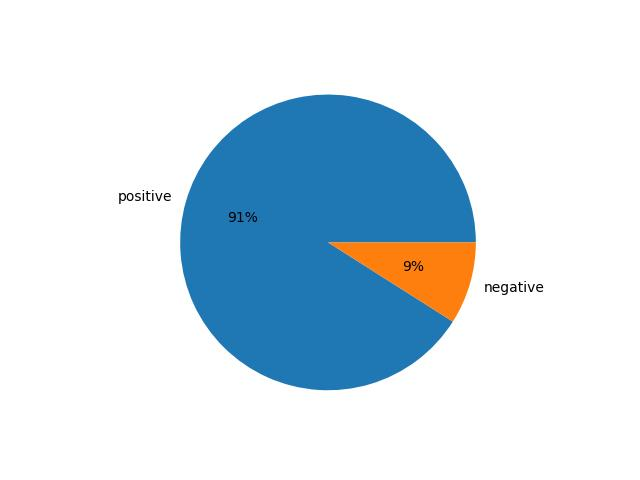
\includegraphics[width=7cm]{figuras/TripAdvisor/Hotels/hotel21_sentiments.jpeg}
\caption{Gráfico circular gerado baseando-se nos \textit{sentiments} dados da plataforma \textit{TripAdvisor} referente à Herdade das Barradas da Serra}
\label{fig:exemplofig21sentimentsTrip}
\end{figure}

\begin{figure}[!htb]
\centering
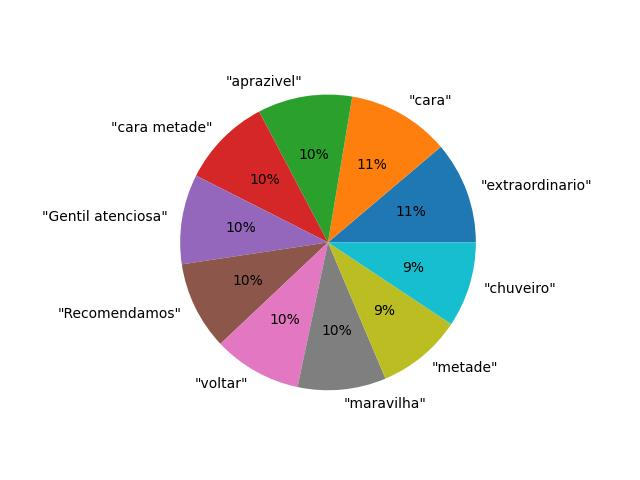
\includegraphics[width=7cm]{figuras/TripAdvisor/Hotels/hotel21_keywords.jpeg}
\caption{Gráfico circular gerado baseando-se nas \textit{keywords} mais usadas da plataforma \textit{TripAdvisor} referente à Herdade das Barradas da Serra}
\label{fig:exemplofig21keywordsTrip}
\end{figure}

\begin{figure}[!htb]
\centering
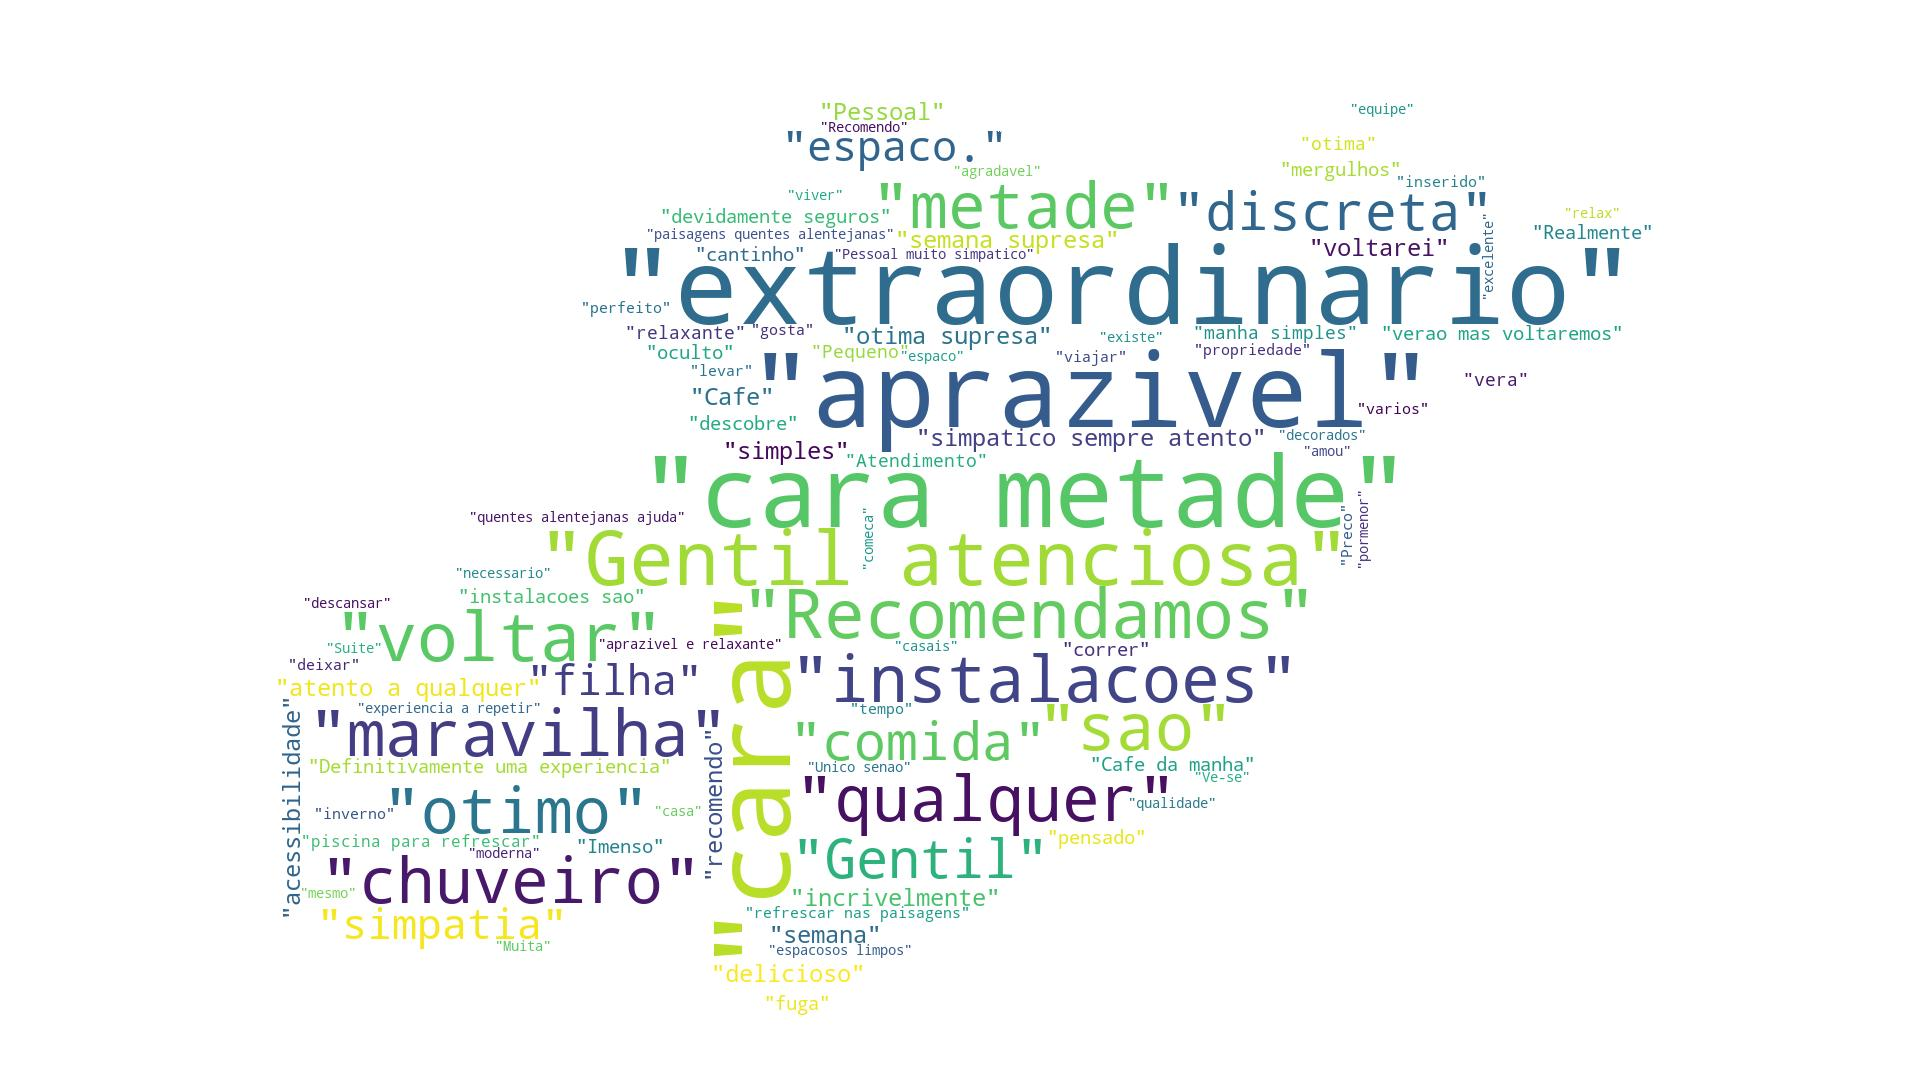
\includegraphics[width=7cm]{figuras/TripAdvisor/Hotels/hotel21_keywordcloud.jpeg}
\caption{Gráfico de \textit{keywords} e nuvens de \textit{keywords} contendo as \textit{keywords} mais usadas da plataforma \textit{TripAdvisor} referente à Herdade das Barradas da Serra}
\label{fig:exemplofig21cloudTrip}
\end{figure}


\section{Gráficos temporais}

Com gráficos temporais, queremos dizer que nos dados apresentados e nas análises é considerado o desenvolvimento temporal, quer isto dizer que as \textit{reviews} mostradas ao longo do tempo tornam possível verificar as datas em que foram escritas e a quantidade que cada hotel/restaurante/atracção recebeu ao longo dos anos e meses.

\subsection{Metodologia}

Para a geração dos gráficos temporais, foi utilizado o \textit{software PowerBI}, que utilizava os ficheiros .csv gerados e organizados previamente vindos da base de dados, contendo todas as informações em ficheiros únicos.
Os gráficos gerados são: gráficos circulares e de tabelas. Os quais demonstram a quantidade de \textit{sentiments} e \textit{keywords} usadas ao longo do tempo por cada hotel, divididos por anos e meses e também por cada hotel.

\subsection{Execução}

Os ficheiros \textit{.csv} que contêm as informações relativas a todas as \textit{keywords} e \textit{sentiments}, foram importados para o \textit{software PowerBI} e posteriormente organizados da maneira que o grupo achou mais conveniente para que os gráficos ficassem o mais apresentáveis e visivelmente mais fáceis para analisar os dados. Posteriormente os gráficos circulares e de tabelas foram exportados para \textit{.jpg} e guardados. 

\subsection{Resultados}

Como se podem verificar nestas três imagens (figura: \cite{fig:exemplofigqntsntmyear},  figura: \cite{fig:exemplofigqntyearbus}, figura: \cite{fig:exemplofigposneg}), os gráficos temporais apresentam um desenvolvimento de \textit{sentiments} e \textit{keywords} ao longo do tempo bastante positivo revelando-se um óptimo ponto para o nosso turismo e \textit{keywords} que mostram bastante agrado. 

\begin{figure}[!htb]
\centering
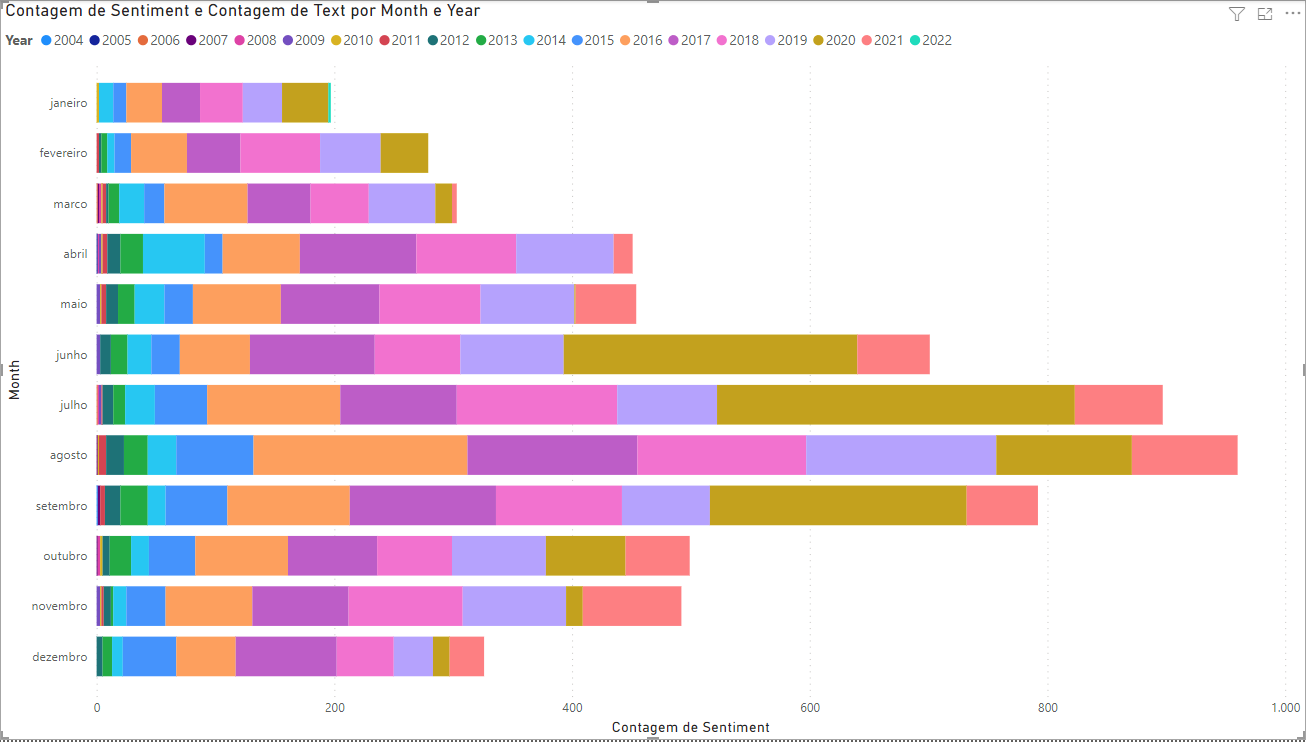
\includegraphics[width=7cm]{figuras/NrReviewsPerYear/TableGraph6.PNG}
\caption{Gráfico de tabelas gerado baseando-se em todos os \textit{sentiments} dados da plataforma \textit{TripAdvisor} ao longo dos anos}
\label{fig:exemplofigqntsntmyear}
\end{figure}

\begin{figure}[!htb]
\centering
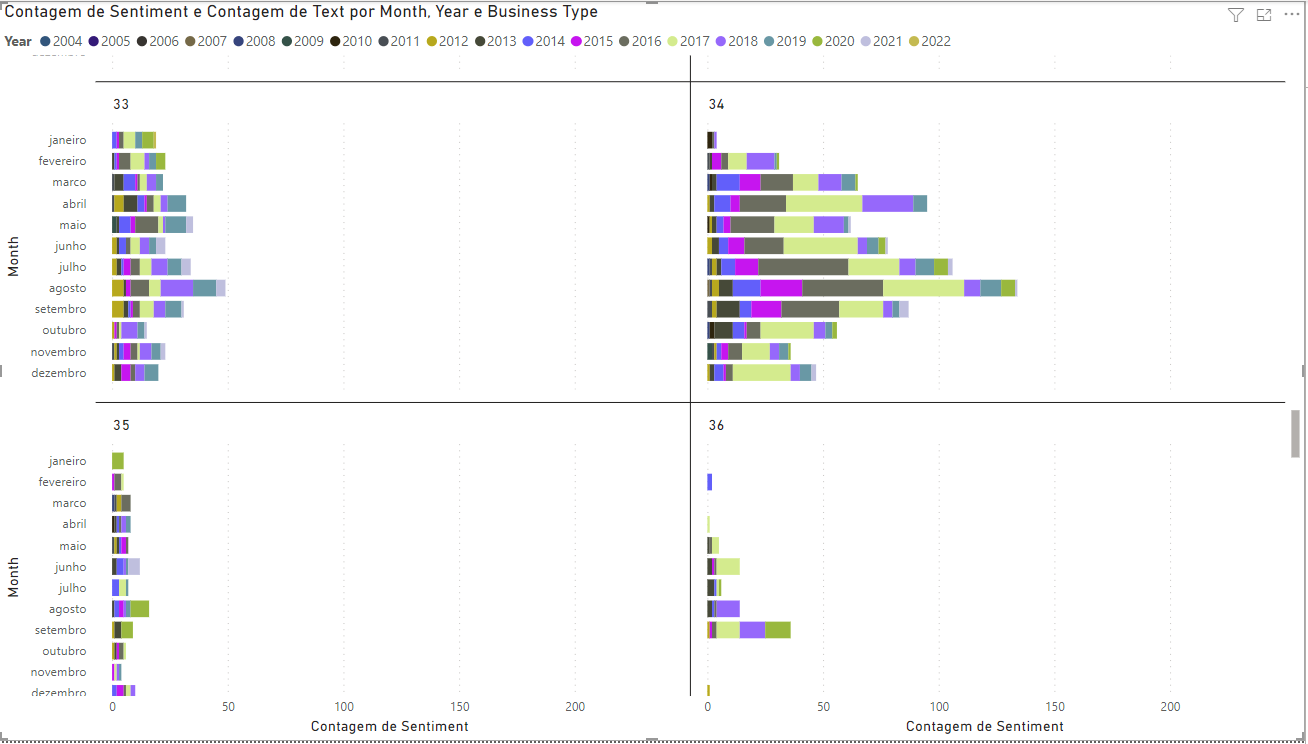
\includegraphics[width=7cm]{figuras/NrReviewsPerYear&BusinessType/8.PNG}
\caption{Gráfico de tabelas gerado baseando-se em todos os \textit{sentiments} da plataforma \textit{TripAdvisor} referente a cada hotel com o decorrer dos anos}
\label{fig:exemplofigqntyearbus}
\end{figure}

\begin{figure}[!htb]
\centering
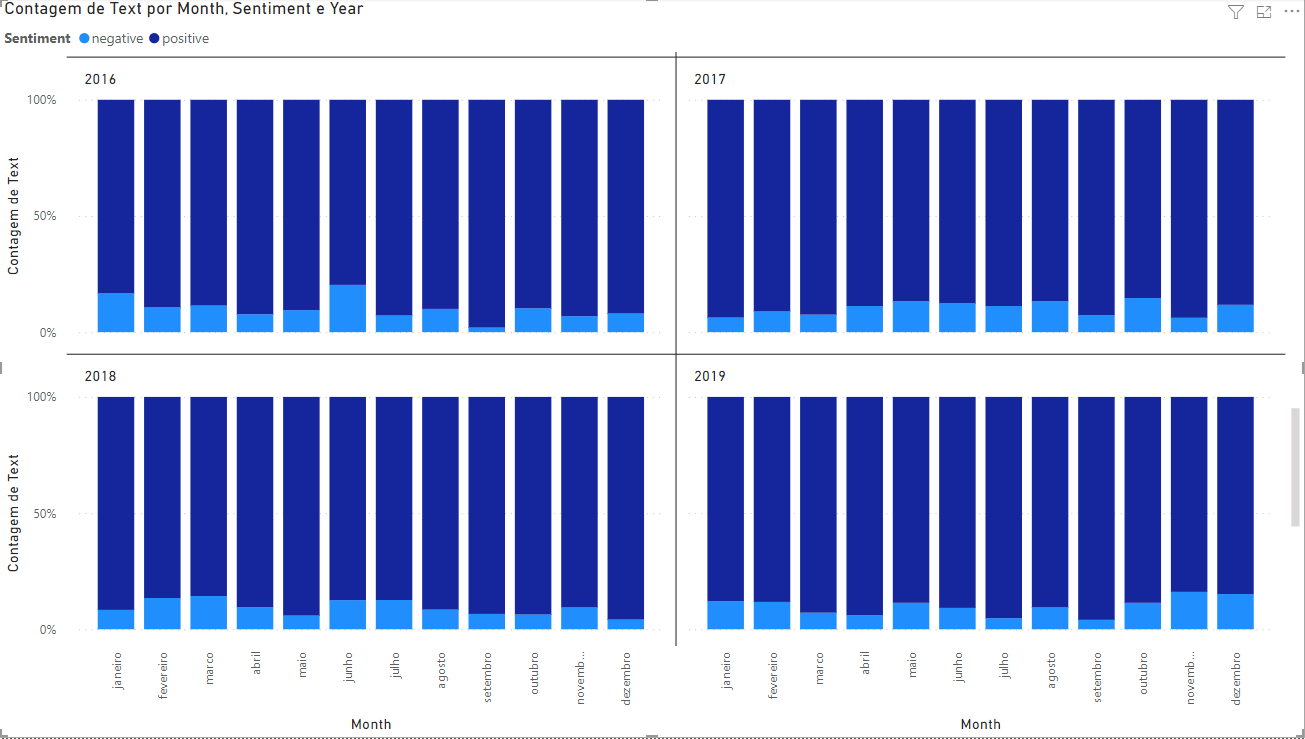
\includegraphics[width=7cm]{figuras/Pos&NegSentiments/TableGraph4.PNG}
\caption{Gráfico de tabelas gerado baseando-se na quantidade de \textit{sentiments} da plataforma \textit{TripAdvisor} positivos e negativos ao longo do tempo para cada hotel}
\label{fig:exemplofigposneg}
\end{figure}
\chapter{Reorganização e DB storage}
\label{cap8}

\section{Reorganização dos dados (\textit{TripAdvisor} apenas)}

Para as analises temporais e para o transporte de dados, foi necessário criar uma base de dados organizada e relacional, que garantisse a integridade dos dados e a sua coerência.

Para isso foram usados os pacotes \textit{pandas} para o \textit{import} dos \textit{.csv} em \textit{DataFrames} e \textit{sqlite3} para a criação da base de dados \textit{SQLite3}.

\subsection{Metodologia}

Inicialmente, foi criada uma base de dados \textit{SQLite3}, que será usada para armazenar os dados. A base de dados \textit{SQLite3} foi criada e as tabelas foram criadas, com os campos correspondentes a cada coluna do ficheiro \textit{.csv}, dos quais os dados foram importados via \textit{pandas}. 

Os \textit{DataFrames} de \textit{pandas} oferecem uma maneira de aceder e manipular dados, e também fornecem uma maneira de criar e manipular tabelas. Todas as operações de manipulação de dados são feitas através de funções de \textit{DataFrame}.

Seguidamente, é empurrado os dados dos \textit{DataFrames} correspondentes às tabelas para a base de dados. Com esta base de dados, é possível fazer consultas e manipulações de dados, tal como também exportar os dados organizados para ficheiros \textit{.csv} de forma a que possam ser usados em outros programas, tais como o \textit{R}, o \textit{Excel}, o \textit{PowerBI}, etc.

\subsection{Execução e Resultados}

Foi feito um \textit{script} para executar a criação da base de dados \textit{SQLite3}, e para o \textit{import} dos dados dos \textit{DataFrames} para a base de dados. O qual foi executado com sucesso, como podemos ver na base de dados e nos ficheiros \textit{.csv}.



\chapter{Análise dos dados obtidos}
\section{Resultados obtidos}

Tendo em vista os gráficos gerados por meio das bibliotecas \textit{MatplotLib, Wordcloud} e também os do \textit{software PowerBI}  foi possível reunir um grande conjunto de informação para realizar uma análise dos melhores pontos turísticos que o património cultural alentejano pode oferecer e assim melhorar possíveis pontos negativos e positivos, ou então prever quais as atrações/hóteis/restaurantes que mais cativam os turistas.

Assim sendo, foram gerados gráficos para cada hótel/restaurante/atração dos \textit{websites Tripadvisor, Booking e Zoomato} usando as bibliotecas mencionadas com o intuito dos resultados serem mais facilmente visíveis com as \textit{keywords} mais usadas para mencionar cada um dos pontos turísticos, assim como um mapa da cidade de Beja que contem todas as \textit{keywords} e as percentagens entre \textit{sentiments} positivos e negativos.

Por fim foram gerados também gráficos com as informações ao longo do tempo dos mesmos \textit{websites} referidos, acerca dos \textit{sentiments} de cada ponto turístico utilizando o \textit{software PowerBI}.

\newpage
\subsection{Resultados de totais}

\begin{figure}[!htb]
\centering
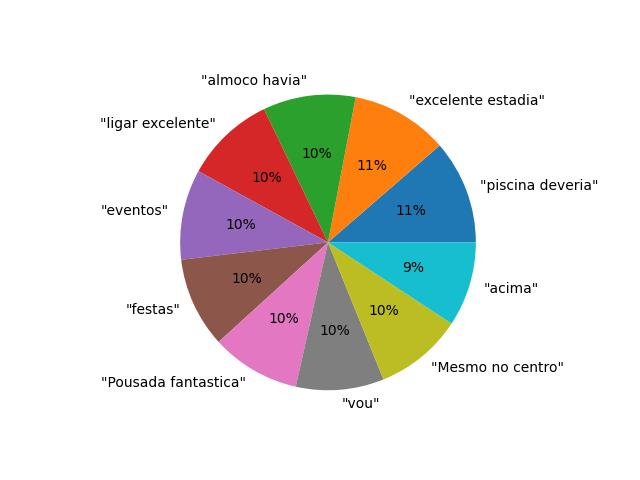
\includegraphics[width=7cm]{figuras/TripAdvisor/Hotels/hotel0_keywords.jpeg}
\caption{Gráfico circular com as \textit{keywords} mais usadas para o hotel 0}
\label{fig:exemplofig}
\end{figure}

\begin{figure}[!htb]
\centering
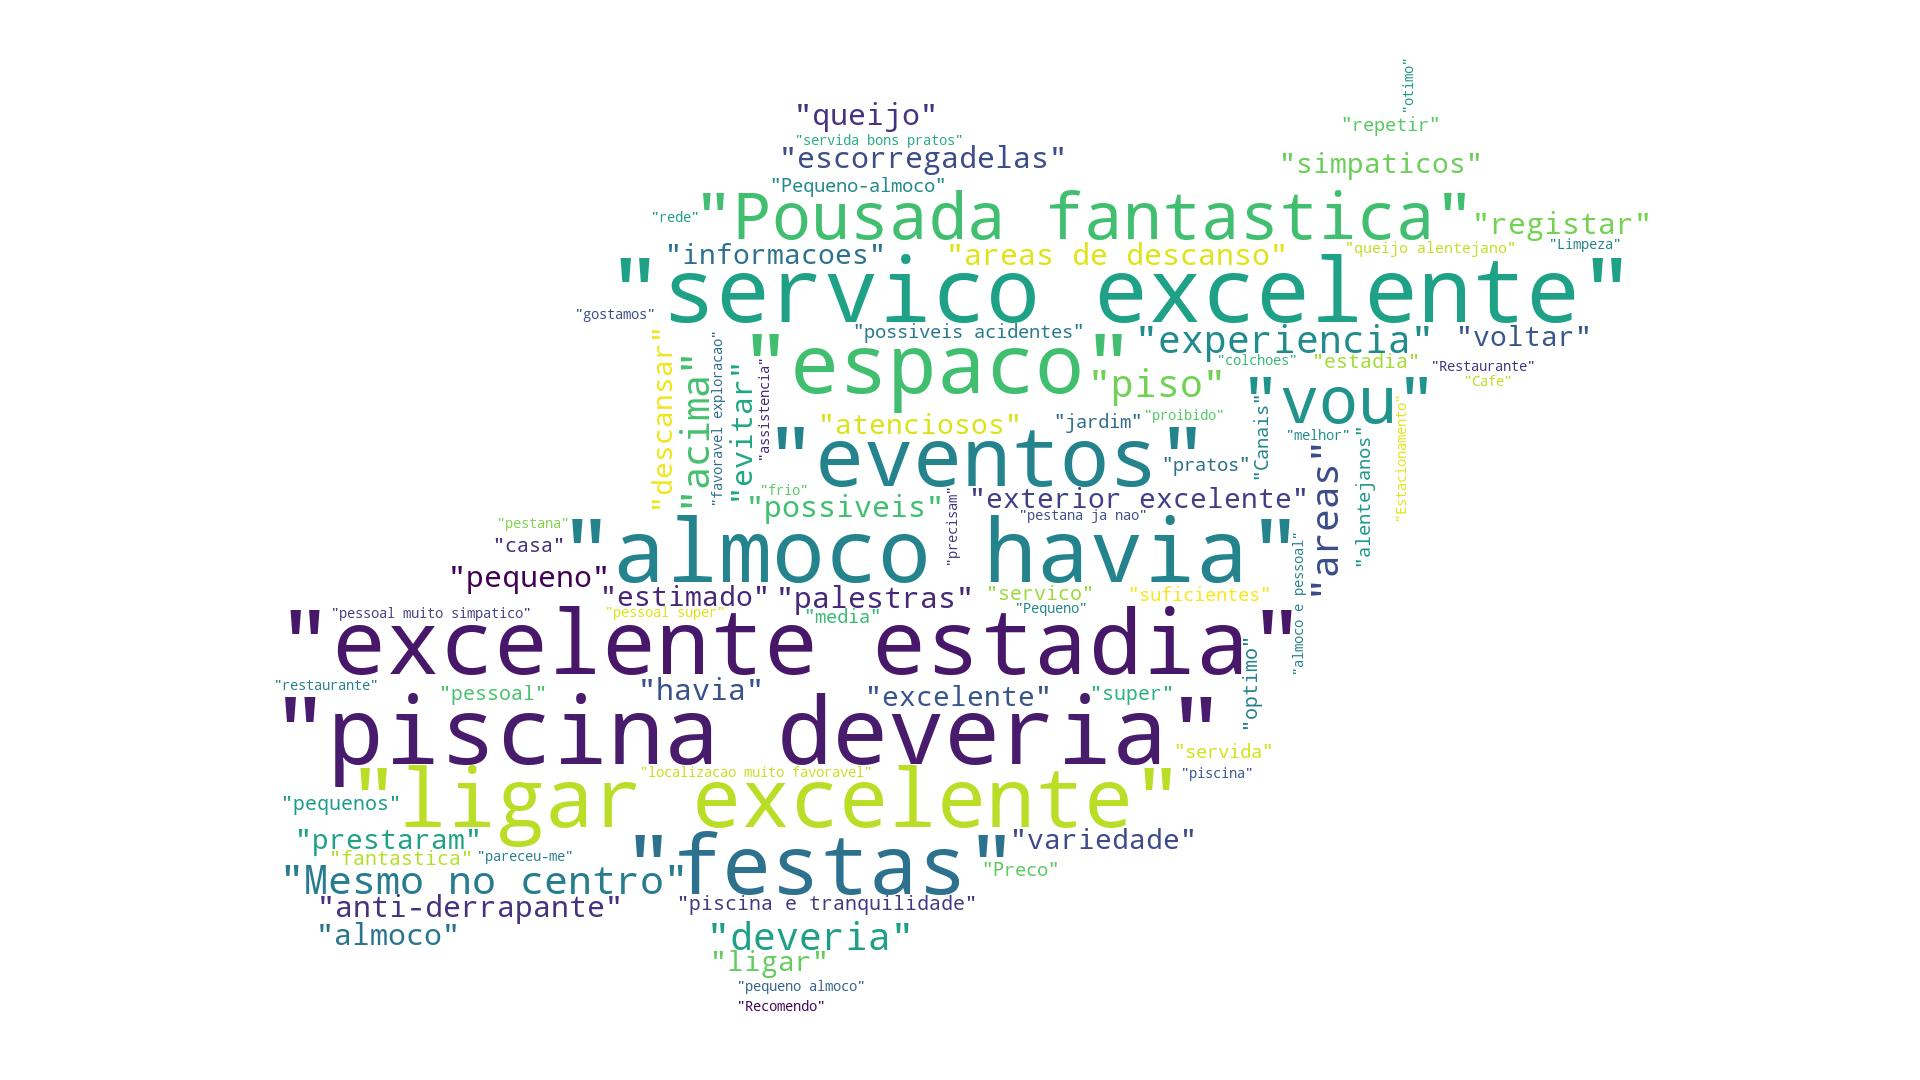
\includegraphics[width=7cm]{figuras/TripAdvisor/Hotels/hotel0_keywordcloud.jpeg}
\caption{Mapa de Beja com as \textit{keywords} mais usadas para o hotel 0 no seu interior}
\label{fig:exemplofig}
\end{figure}

\begin{figure}[!htb]
\centering
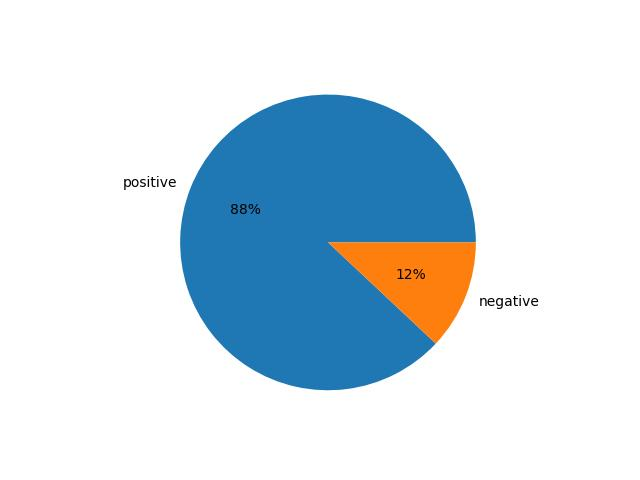
\includegraphics[width=7cm]{figuras/TripAdvisor/Hotels/hotel0_sentiments.jpeg}
\caption{Gráfico circular a representar a diferença entre os \textit{sentiments} positivos e negativos}
\label{fig:exemplofig}
\end{figure}

\newpage

Nas figuras apresentadas acima são mostrados alguns resultados gerados pelas bibliotecas mencionadas, dos quais podemos notar que existe uma maioria para a quantidade de \textit{sentiments} positivos em relação aos negativos e que a maior parte das \textit{keywords} são também positivas. Porém, estes valores são retirados no momento em que a extração dos dados foi realizada e não é possível verificar à medida do tempo como esses valores foram surgindo. Os valores entre restaurantes/hóteis/atrações é bastante semelhante entre si e então foi decidido que só iria ser mostrado alguns exemplos da realização desta etapa e todos os resultados ficariam mostrados nos anexos.

\subsection{Resultados temporais}

\begin{figure}[!htb]
\centering
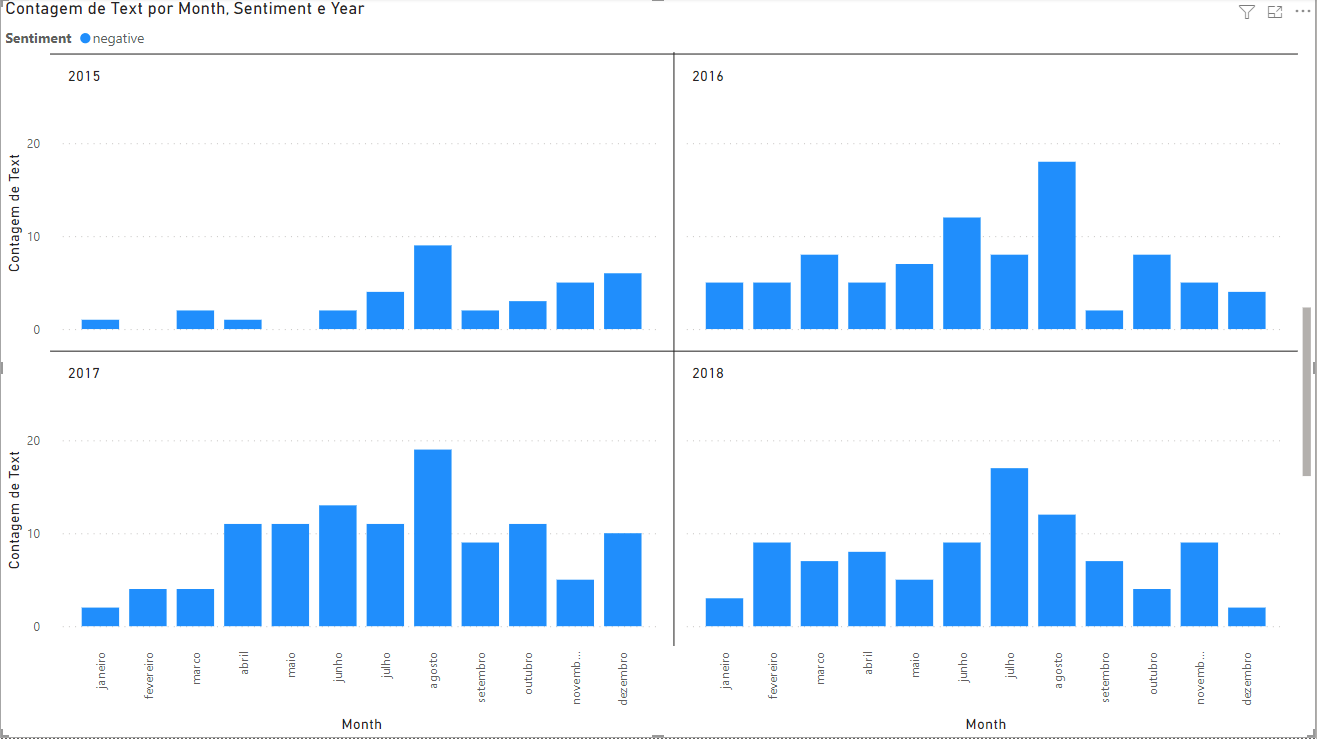
\includegraphics[width=12cm]{figuras/NegPerYear/1.PNG}
\caption{Gráfico de tabelas com a quantidade de \textit{sentiments} negativos ao longo do ano de cada hótel}
\label{fig:exemplofig}
\end{figure}

\begin{figure}[!htb]
\centering
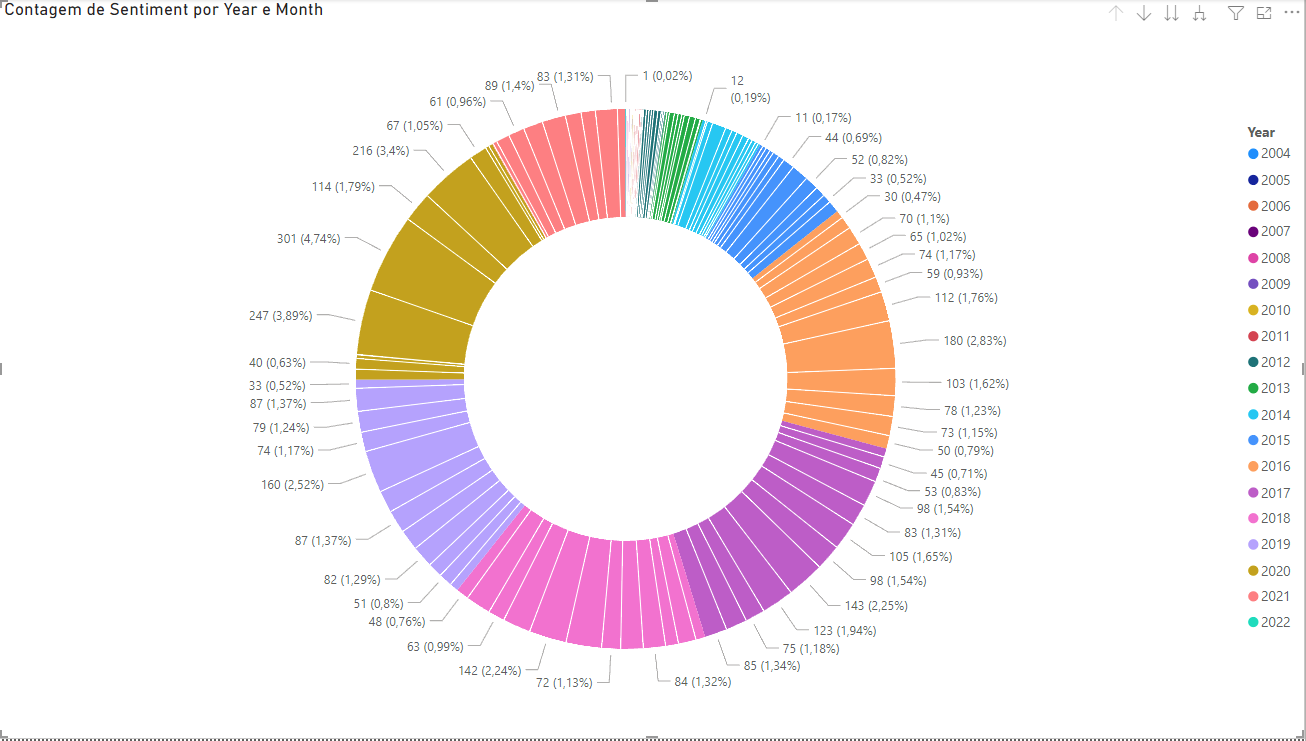
\includegraphics[width=12cm]{figuras/NrReviewsPerYear/CircleGraph.PNG}
\caption{Gráfico circular com a quantidade de \textit{reviews} ao longo do ano}
\label{fig:exemplofig}
\end{figure}

\begin{figure}[!htb]
\centering
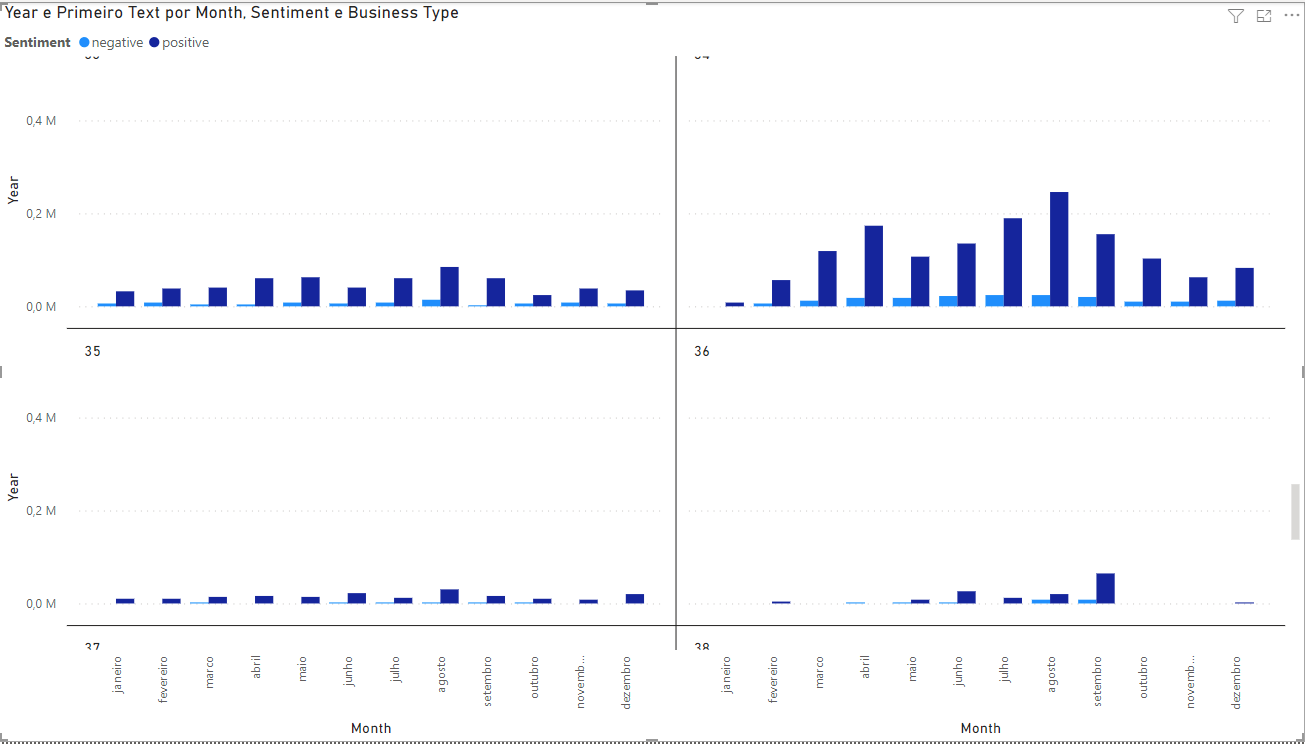
\includegraphics[width=12cm]{figuras/Pos&NegSentimentsPerMonth&BusinessType/2.PNG}
\caption{Gráfico de tabelas com a quantidade de \textit{sentiments} ao longo do ano por cada estabelecimento}
\label{fig:exemplofigNeg}
\end{figure}

\newpage
As figuras apresentadas desta vez foram elaboradas com o valor temporal bastante visível, sendo possível verificar desta vez uma evolução com o decorrer do tempo dos valores apresentados, assim como a forte diferença entre a quantidade de \textit{sentiments} escritos em meses onde um grande número de pessoas adere aos serviços, como no verão, Páscoa ou Natal.
\newpage

\section {Análise dos resultados}

Graças a estes gráficos podemos concluir que as opiniões acerca do turismo cultural na zona alentejana é bastante positiva, mostrando uma enorme maioria de comentários positivos contra uma pequena quantidade de comentários negativos (Figura: \ref{fig:exemplofigNeg}). Podemos também notar que existem muitas mais pessoas a dar as sua opiniões em meses como junho, julho e agosto, muito possivelmente devido á abertura das épocas balneares que movem grandes grupos de turistas nacionais e estrangeiros a fazerem férias pelas zonas costeiras que o Alentejo consegue fornecer com enorme facilidade graças ás magnificas praias na sua zona costeira. Por fim também é possível notar a evolução no número de opiniões com o decorrer dos anos e com a popularidade que o \textit{website} vai conseguindo, já que no começo o número de opiniões é baixo, porem com o passar dos anos começa a subir em elevado número.

É interessante também realçar um detalhe acerca de um gráfico em específico que o grupo decidiu não passar em branco. O gráfico da figura \ref{fig:exemplofigStrange}.

\begin{figure}[!htb]
\centering
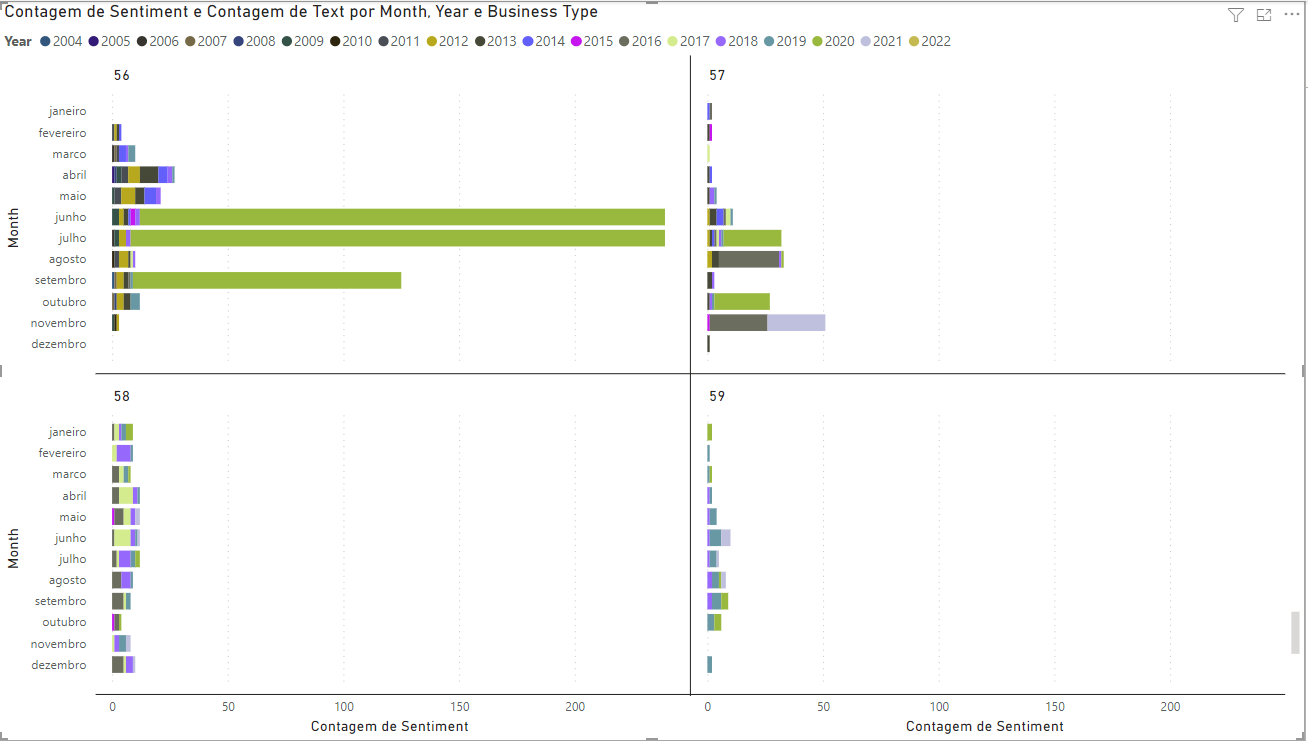
\includegraphics[width=12cm]{figuras/NrReviewsPerYear&BusinessType/9.PNG}
\caption{Gráfico de tabelas com a quantidade de \textit{sentiments} ao longo do ano por cada estabelecimento com valores diferentes}
\label{fig:exemplofigStrange}
\end{figure}

O estabelecimento com o número 56 contém valores interessantes nos meses de junho e julho. São interessantes uma vez que durante o ano de 2020 o país se encontrava em confinamento devido á COVID-19, não sendo possível que ajuntamentos fossem realizados, porem foi verificado através do gráfico que o mesmo não se parece verificar já que existe uma brutal subida no número de pessoas a dar a sua opinião acerca da estadia que realizou, o que dá a entender que esse estabelecimento continuou a realizar as suas tarefas com normalidade ao contrário de outros que provavelmente seguiram as normas recomendadas.

\label{cap9}

 \chapter{Conclusão}
\label{cap10}

Uma análise de dados apresenta sempre uma oportunidade de crescimento, em especial num meio de turismo rural (ou semi-rural) em que os habituais clientes podem (e vão) usar redes sociais e plataformas de comentário de prestação de serviço, para agregar dados comportamentais e percepção pública das ofertas turísticas.

Neste trabalho foi apresentado um agregado exemplar desse tipo de dados e análise o qual foi feito na melhor das formas, dado o conhecimento a nós atribuído pela escola e o tempo disponível. O qual apresentou pouco de informação nova, mas colabora com a percepção pública que se sente nos meios de comunicação verbal subjectiva em locais públicos, ou seja, existe a tendência de haver um maior número de clientes durante as típicas alturas de férias, referimos o ano novo, a Páscoa e em especial o verão.

O que foi dito acima foram as tendências observadas na análise dos dados obtidos nos gráficos gerados para análise temporal, com os dados da plataforma mais completa deste estudo, o \textit{TripAdvisor}. O único caso mais em especial, foi a explosão de \textit{reviews} em Junho e Julho de 2020, que coincide com a abertura da época balnear após desconfinamento (COVID-19) no dia 6 de Junho de 2020, que embora fazendo \textit{cross-referencing} com os dados das \textit{keywords} da mesma análise temporal, não nos dê informação relevante, a coincidência é meramente atractiva e oferece uma fácil explicação.

Sendo assim podemos concluir que foi um trabalho bem sucedido, mesmo que não ofereça novos \textit{insights}, mas corrobora as noções e conhecimento público da área, tal como os dados das análises anuais oferecidas pelo \textit{Booking}. Graças a isto obtemos uma noção da metodologia desta área profissional e os nossos avaliados terão uma noção da qualidade de trabalho produzida por nós.

Sumarizamos assim que nesta secção de turismo rural (e semi-rural), da região de Beja, tem por norma uma boa prestação de serviço, ou pelo menos essa noção é transposta na mente popular de quem visita, e que não existem anomalias na distribuição de visitantes nem de tendências sentimentais ao longo do ano nem ao longo das décadas, mantendo-se previsível mas agradável.

% para adicionar o  capítulo N adicione a linha \input{capituloN} e crie o ficheiro
% capituloN.tex na directoria "capitulos"


%%%%%%%%%%%%%%%%%%%%%%%%%%%%%%%%%%%%%%%%%%%%%%%%
% Bibliografia
\clearpage
\printbibliography[heading=bibintoc]
%%%%%%%%%%%%%%%%%%%%%%%%%%%%%%%%%%%%%%%%%%%%%%%%
\apendices
\chapter{\textit{Jupyter Notebook} da Extração de Palavras-Chave}
\label{ap1}

%a linha seguinte deve ser substituída pelo texto do apêndice

Nas paginas seguintes está incluída uma renderização do \textit{notebook} de \textit{Jupyter} em que se detalha (em inglês) os passos das rotinas de extracção de palavras-chave, comentando de forma simples o funcionamento das funções de código usadas.

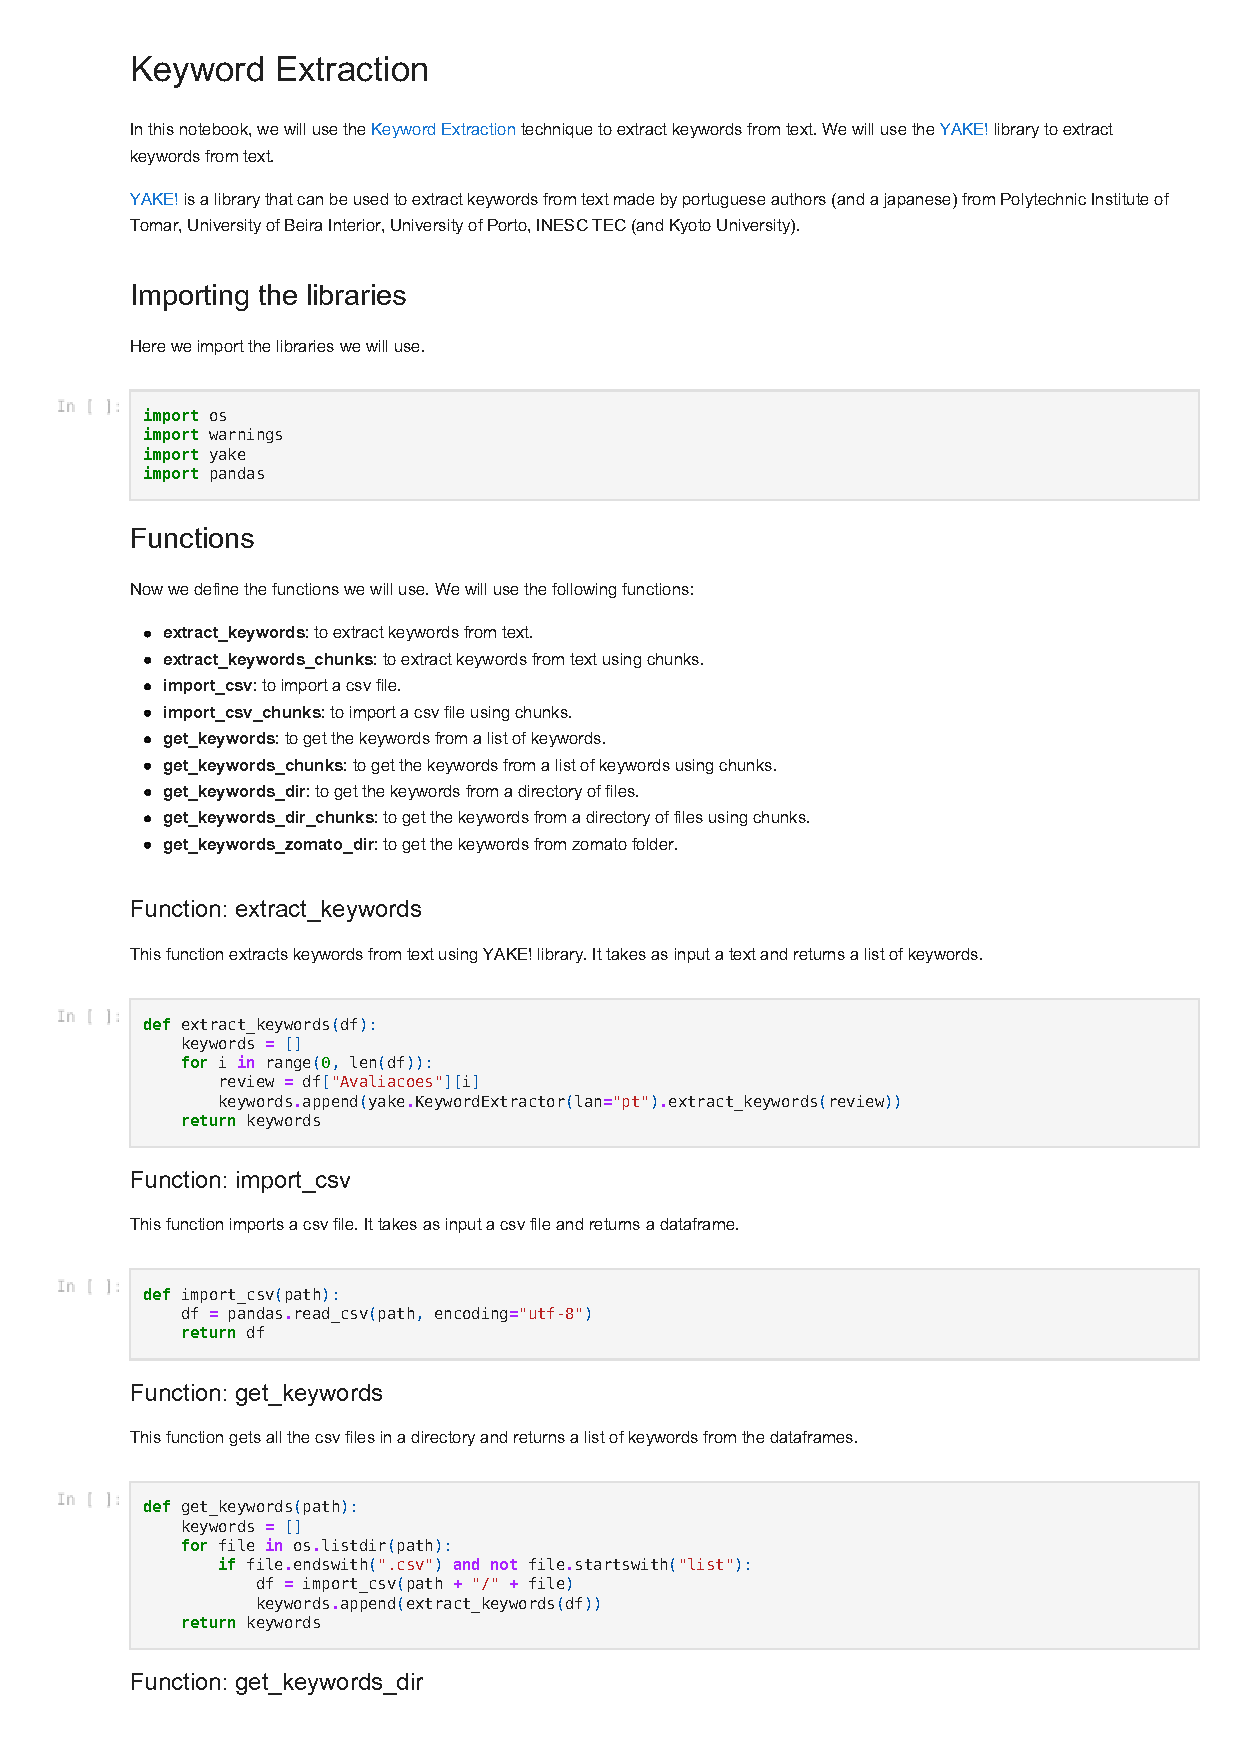
\includepdf[pages=-2,scale=0.75]{jupyter/ta-kwe.pdf}
\chapter{\textit{Jupyter Notebook} da Analise de Sentimentos via \textit{Naïve Bayes Classifier}}
\label{ap2}

%a linha seguinte deve ser substituída pelo texto do apêndice

Nas paginas seguintes está incluída uma renderização do \textit{notebook} de \textit{Jupyter} em que se detalha (em inglês) os passos das rotinas de extracção de palavras-chave, comentando de forma simples o funcionamento das funções de código usadas.

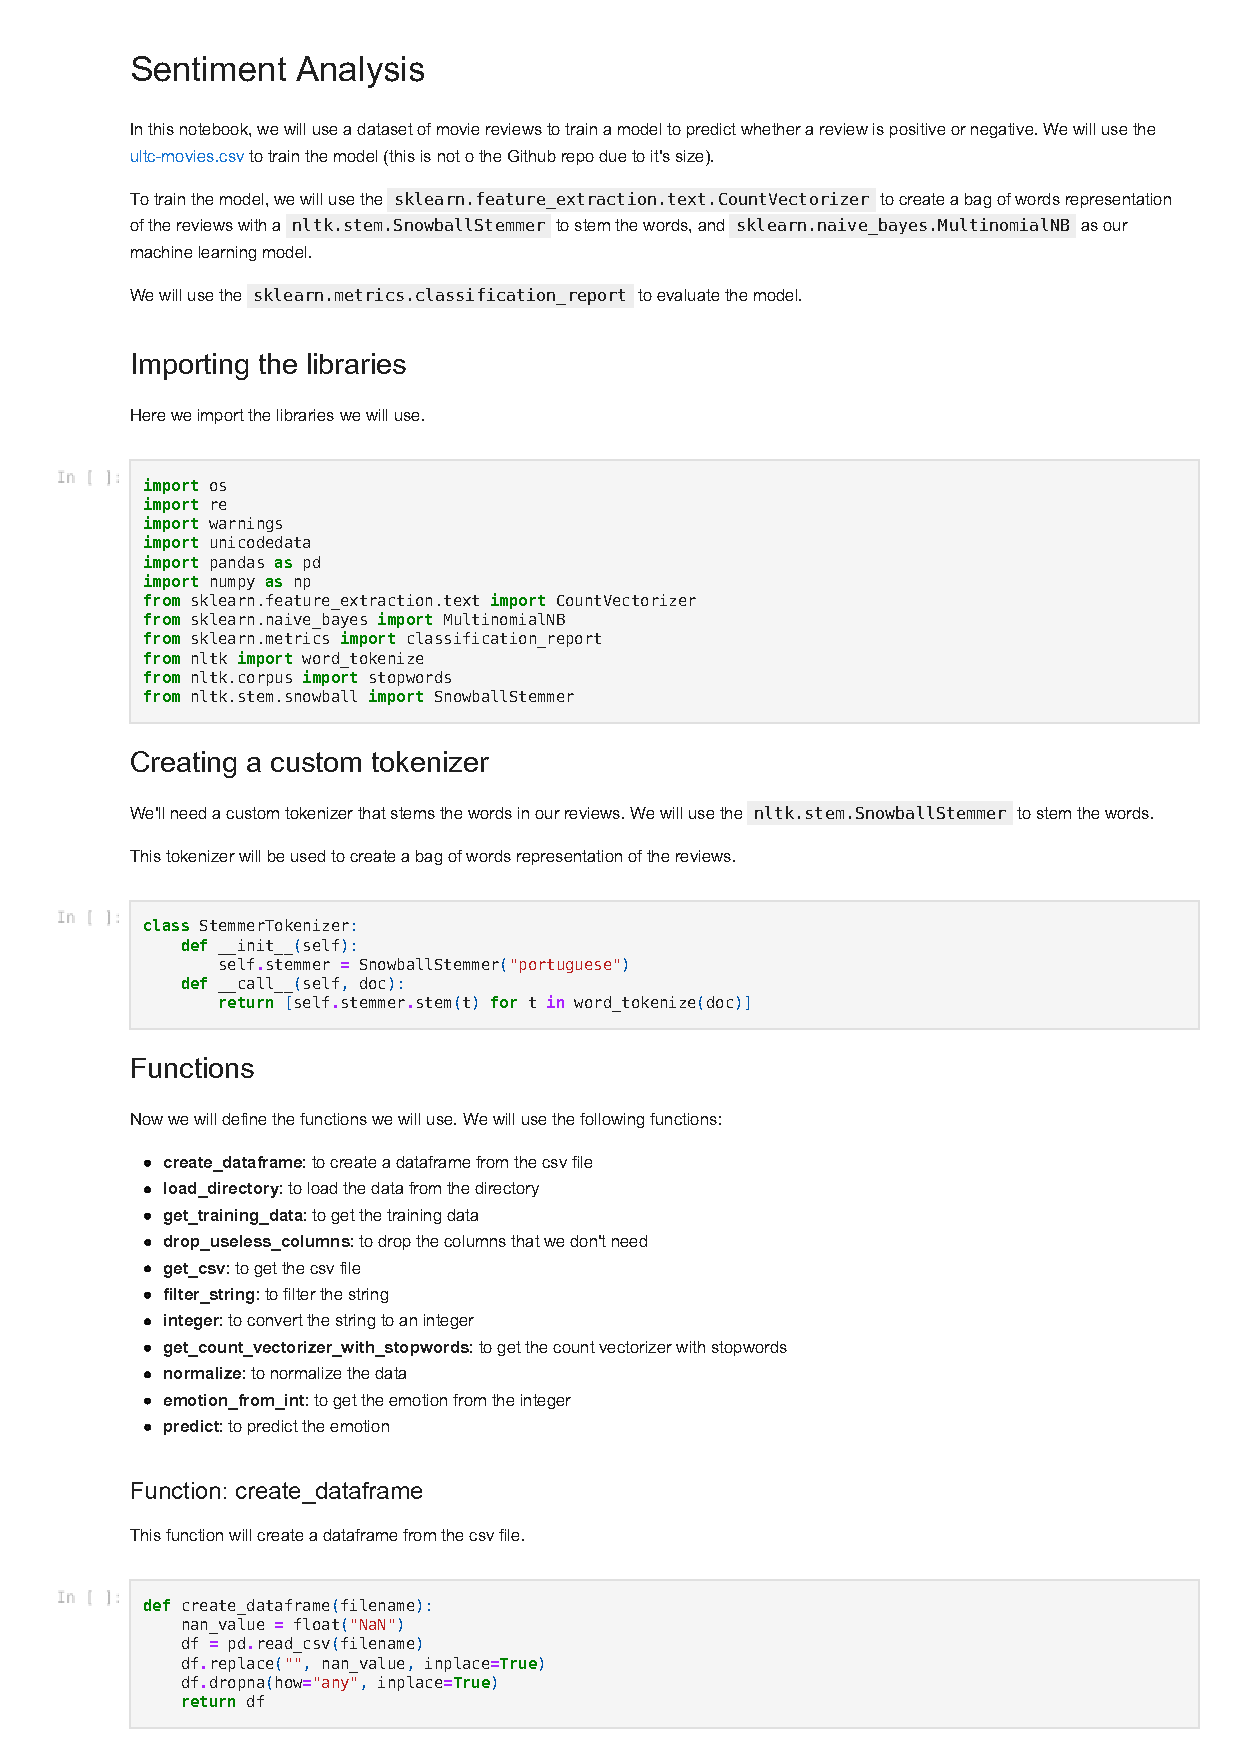
\includepdf[pages=-,scale=0.75]{jupyter/ta-sa-nb.pdf}
\chapter{\textit{Jupyter Notebook} da Analise de Sentimentos via \textit{BERT Transformer Pipelines}}
\label{ap3}

%a linha seguinte deve ser substituída pelo texto do apêndice

Nas paginas seguintes está incluída uma renderização do \textit{notebook} de \textit{Jupyter} em que se detalha (em inglês) os passos das rotinas de extracção de palavras-chave, comentando de forma simples o funcionamento das funções de código usadas.

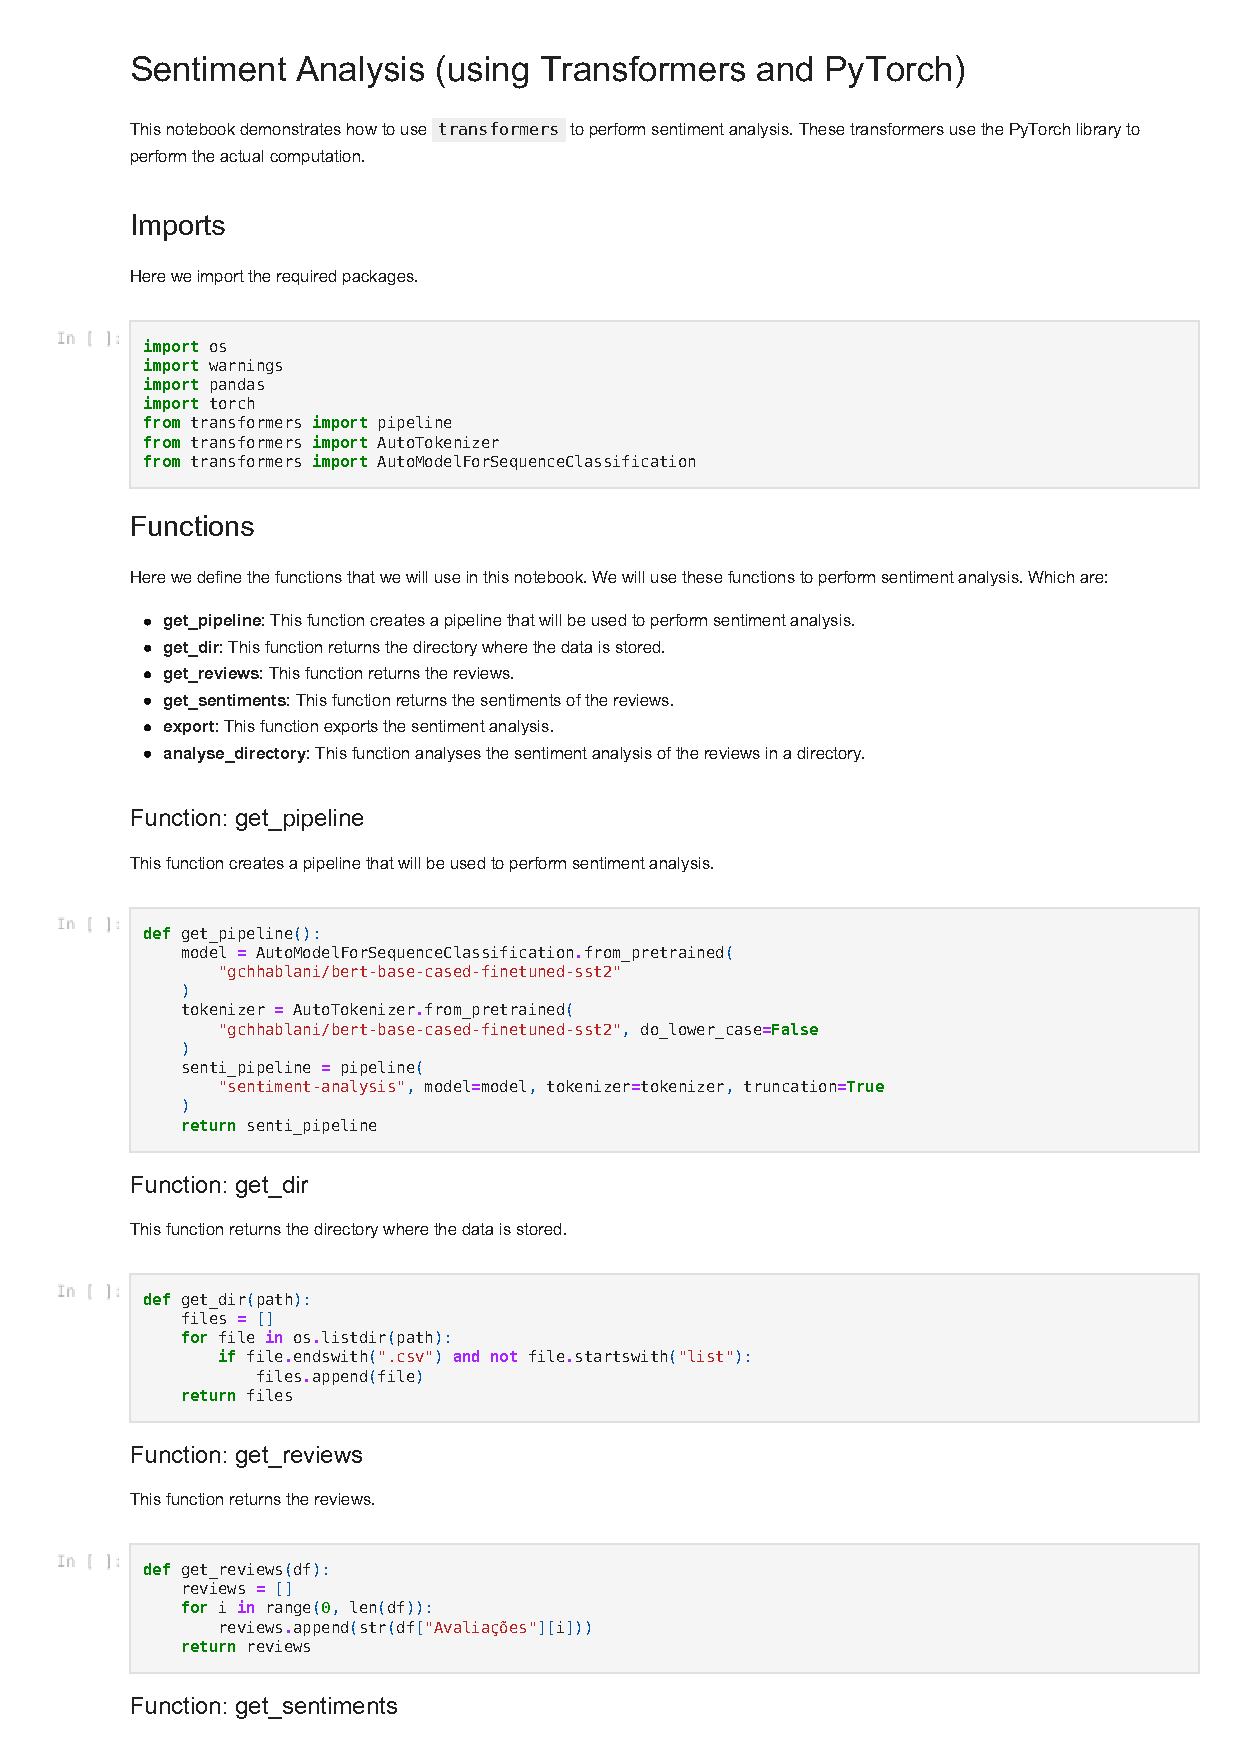
\includepdf[pages=-,scale=0.75]{jupyter/ta-sa-tf.pdf}
\chapter{\textit{Jupyter Notebooks} do \textit{Webscraping} dos hotéis do \textit{Booking}}
\label{ap4}

%a linha seguinte deve ser substituída pelo texto do apêndice

Nas paginas seguintes está incluída uma renderização dos \textit{notebooks} de \textit{Jupyter} em que se detalha (em inglês) os passos das rotinas de extracção de palavras-chave, comentando de forma simples o funcionamento das funções de código usadas.

O primeiro detalha a busca dos hotéis e o segundo apenas os \textit{reviews} de cada um dos hotéis encontrados no primeiro.

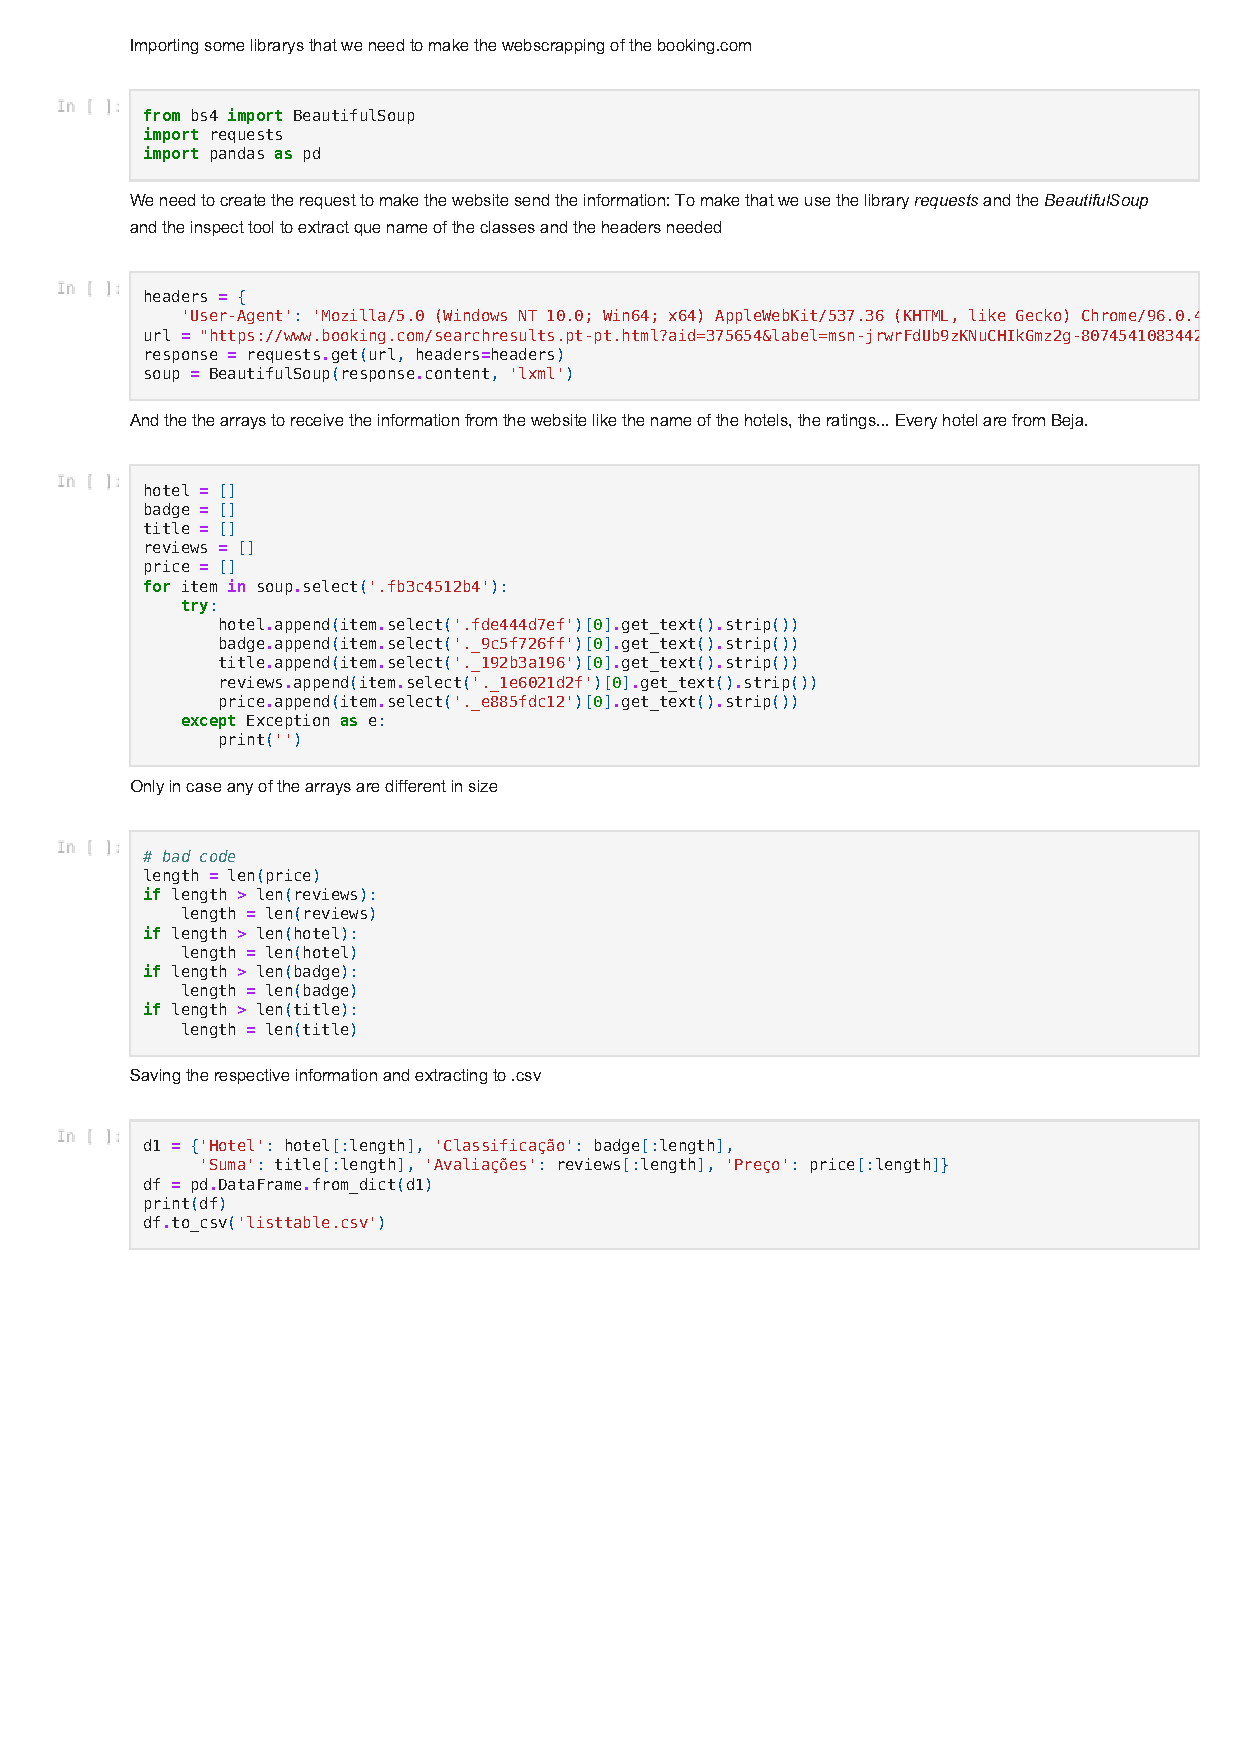
\includepdf[pages=-,scale=0.75]{jupyter/ws-b-h.pdf}
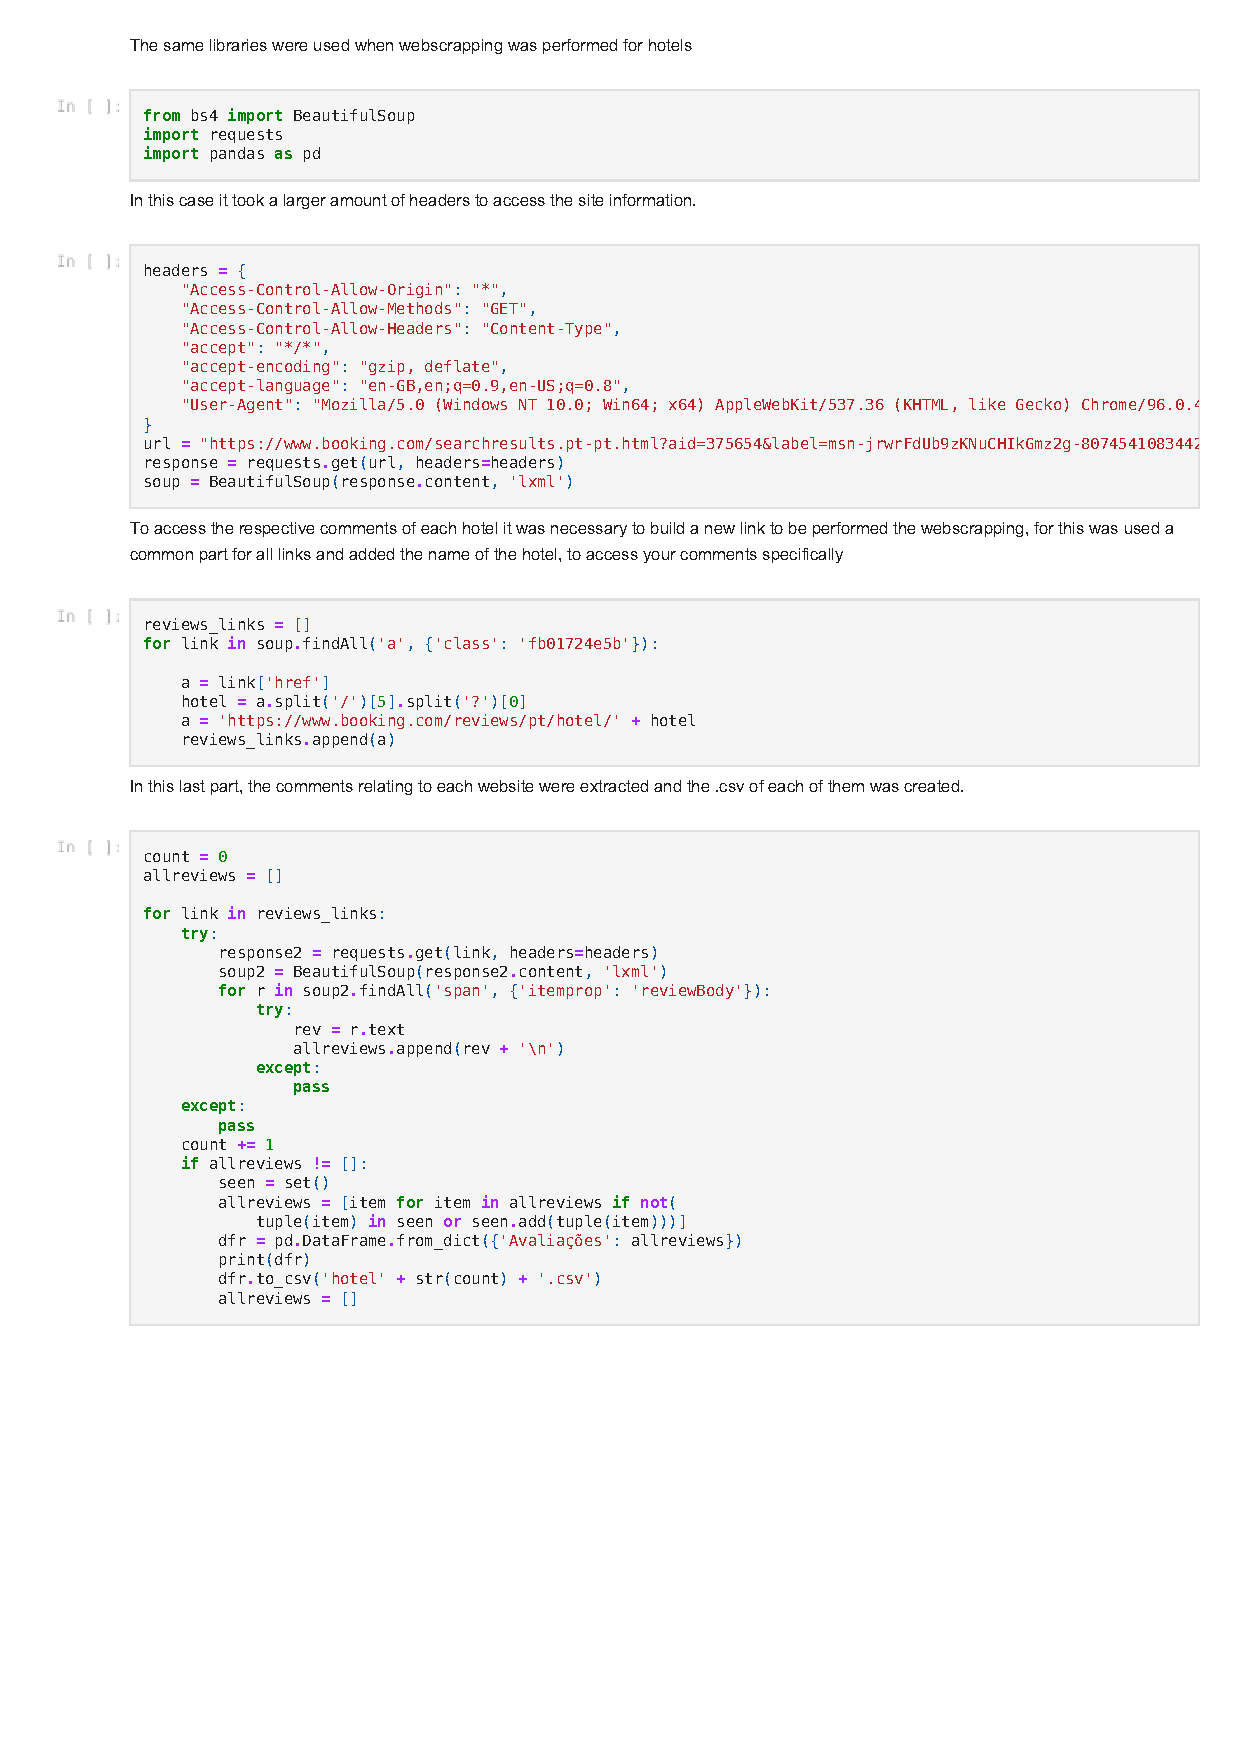
\includepdf[pages=-,scale=0.75]{jupyter/ws-b-h-r.pdf}
\chapter{\textit{Jupyter Notebook} do \textit{Webscraping} dos \textit{reviews} de Restaurantes do \textit{Zomato}}
\label{ap5}

%a linha seguinte deve ser substituída pelo texto do apêndice

Nas paginas seguintes está incluída uma renderização do \textit{notebook} de \textit{Jupyter} em que se detalha (em inglês) os passos das rotinas de extracção de palavras-chave, comentando de forma simples o funcionamento das funções de código usadas.

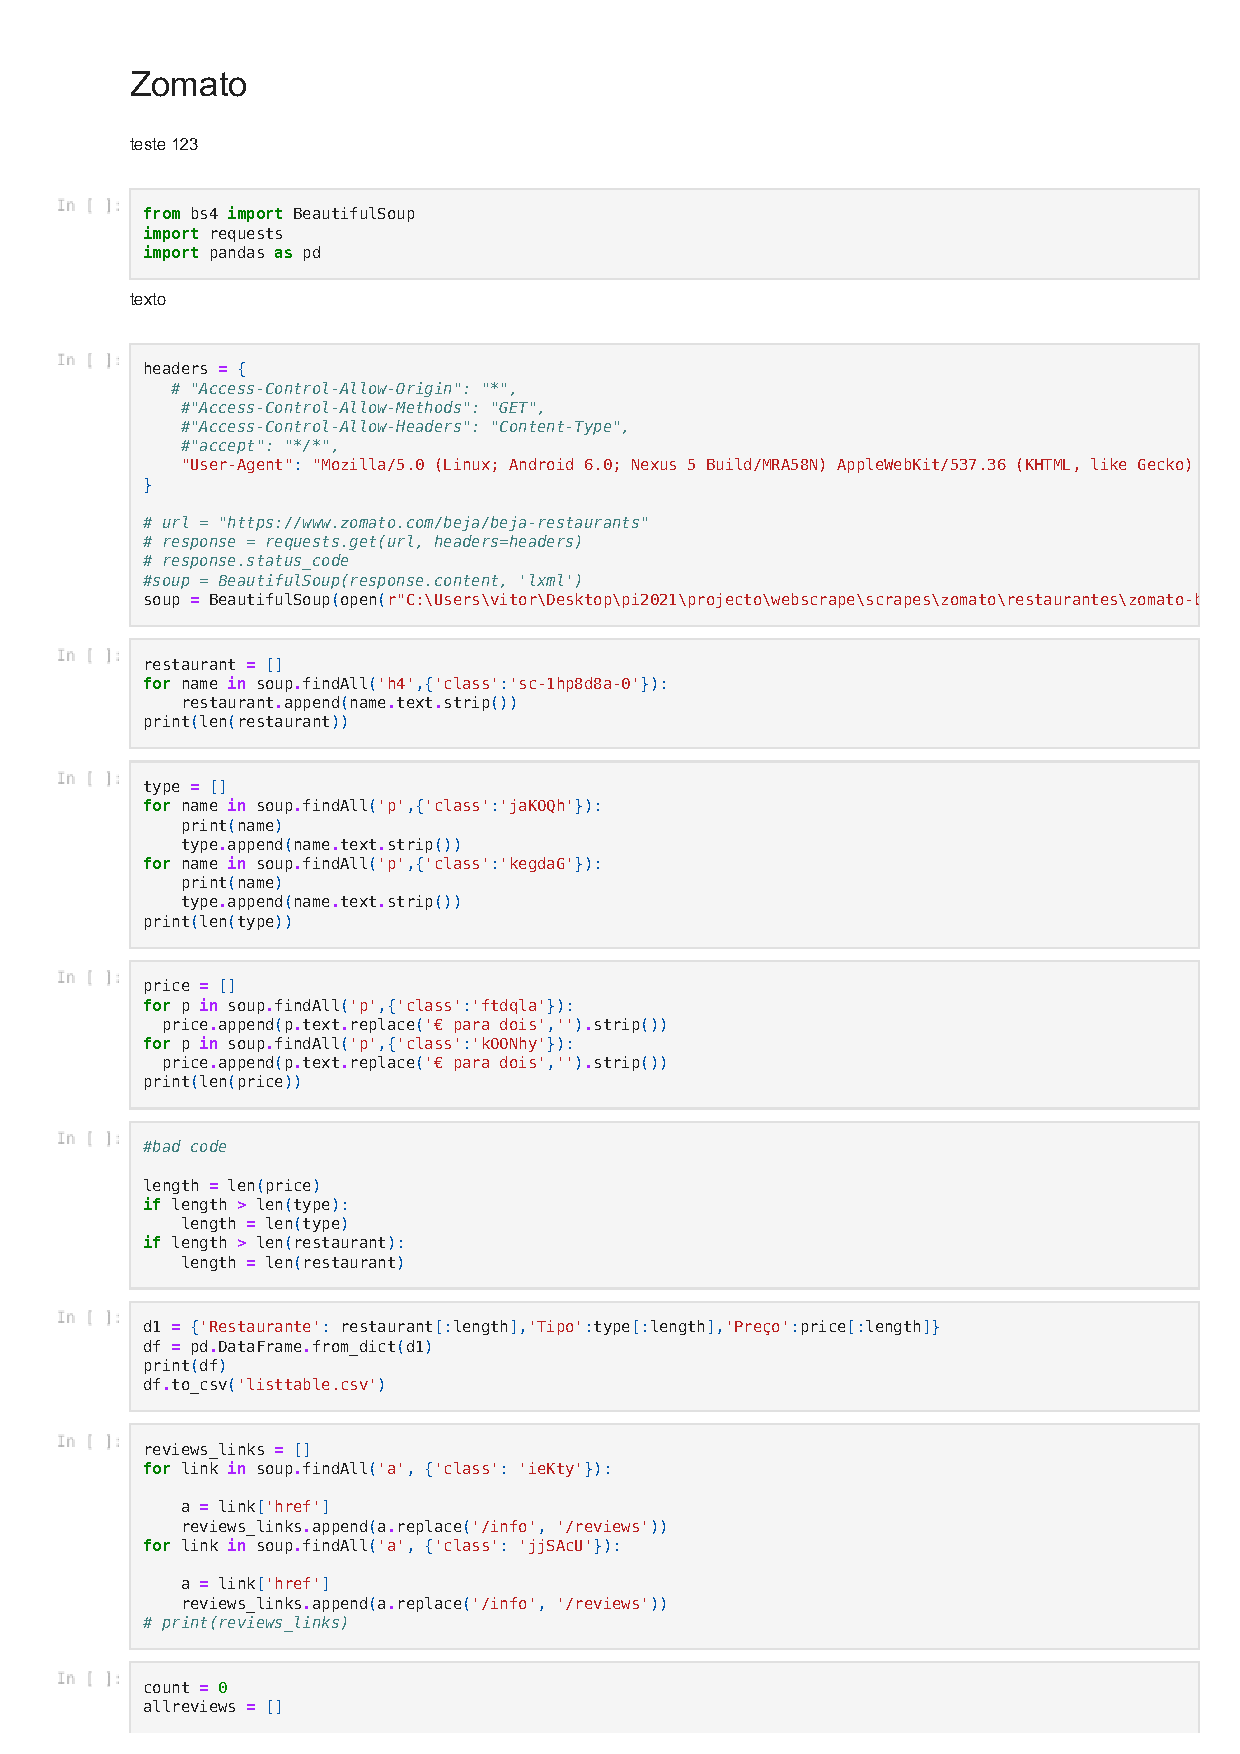
\includepdf[pages=-,scale=0.75]{jupyter/ws-z-r.pdf}
\chapter{\textit{Jupyter Notebooks} do \textit{Webcraping} dos \textit{reviews} dos hotéis, atracções e restaurantes do \textit{TripAdvisor}}
\label{ap6}

%a linha seguinte deve ser substituída pelo texto do apêndice

Nas paginas seguintes está incluída uma renderização dos \textit{notebooks} de \textit{Jupyter} em que se detalha (em inglês) os passos das rotinas de extracção de palavras-chave, comentando de forma simples o funcionamento das funções de código usadas.

O primeiro extraiu os hotéis, o segundo as atracções e o terceiro os restaurantes  (e os seus respectivos \textit{reviews}).

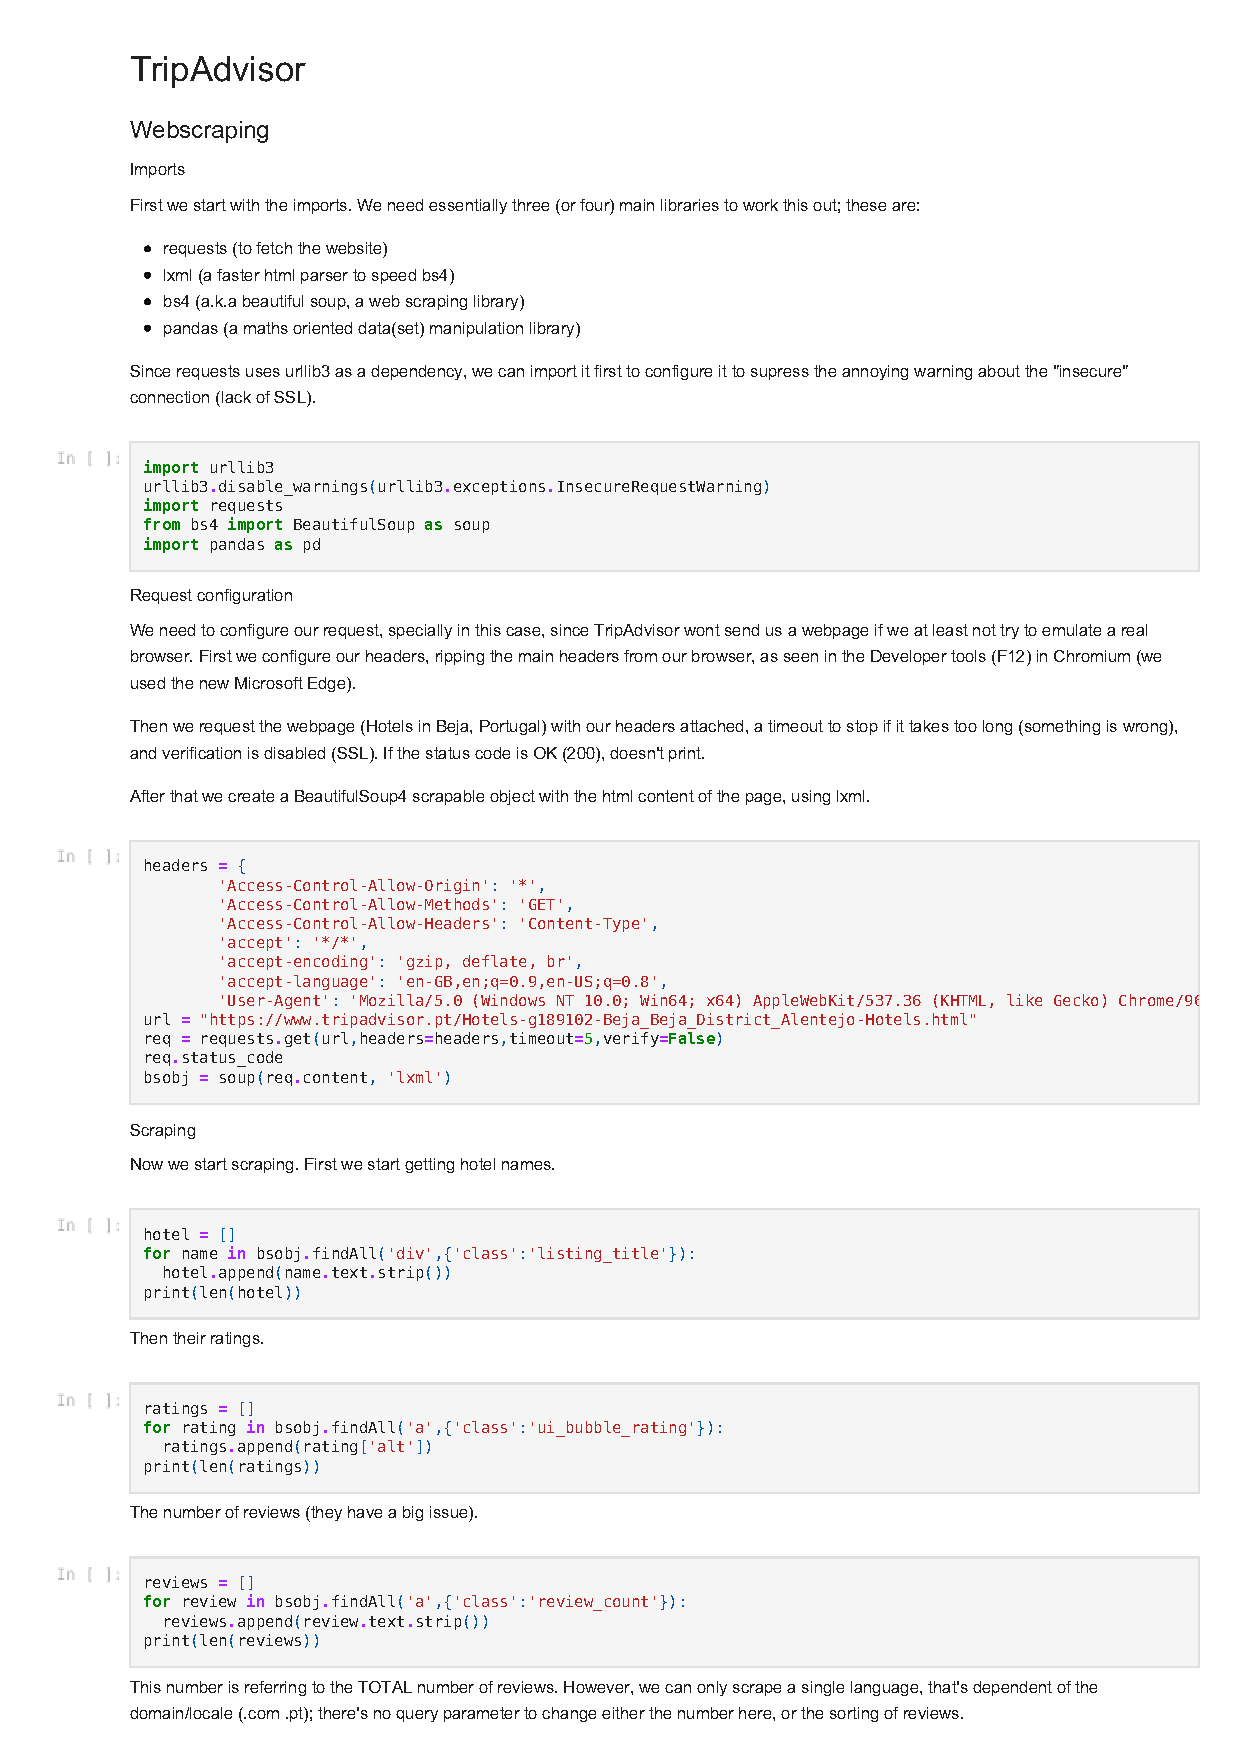
\includepdf[pages=-,scale=0.75]{jupyter/ws-ta-h.pdf}
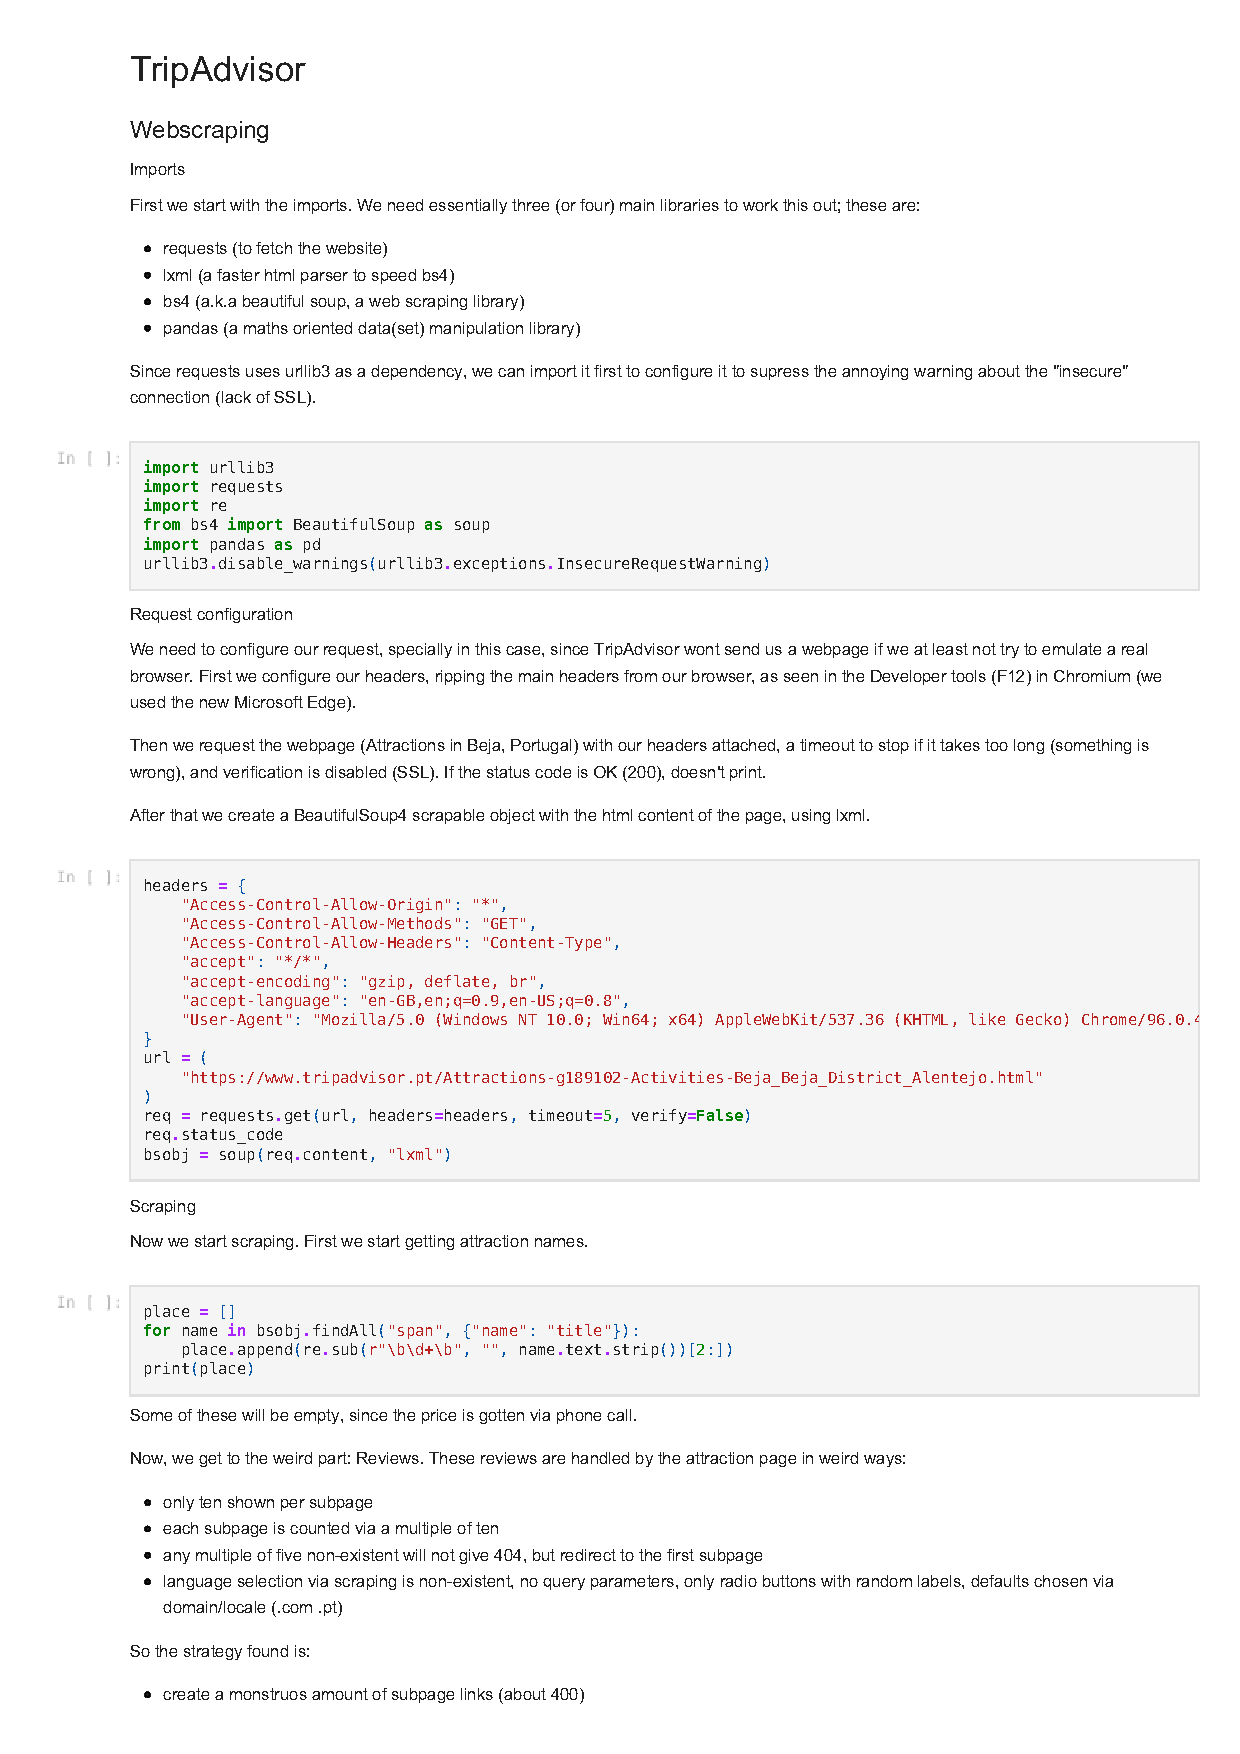
\includepdf[pages=-,scale=0.75]{jupyter/ws-ta-a.pdf}
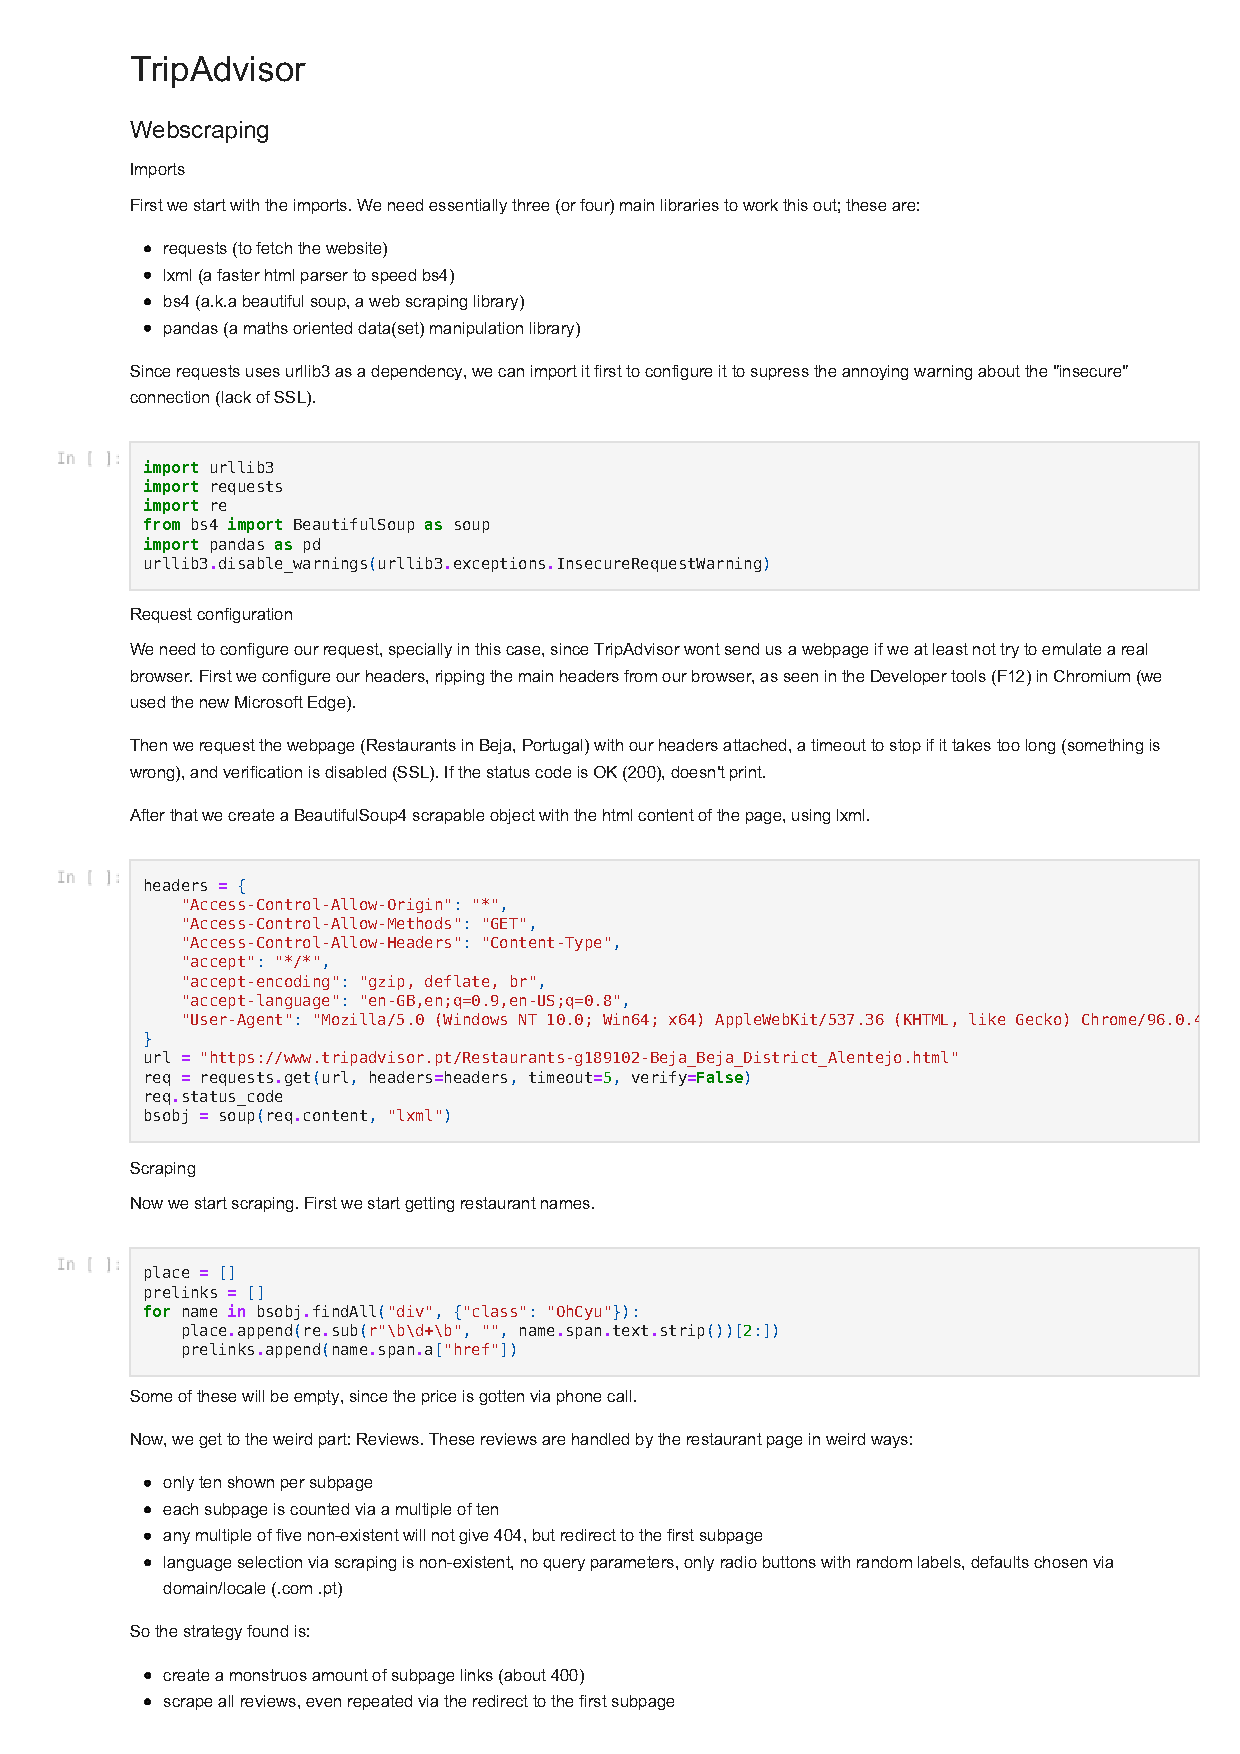
\includepdf[pages=-,scale=0.75]{jupyter/ws-ta-r.pdf}
\chapter{Código do \textit{script} de \textit{Python} que fez o \textit{trimming} dos ficheiros \textit{.csv}}
\label{ap7}

Aqui abaixo está representado o código de \textit{Python} que fez o que fez o \textit{trimming} dos ficheiros \textit{.csv webscraped} para uso posterior sem potenciais erros.

\begin{minted}[linenos,tabsize=2,breaklines,breakanywhere]{python3}
import os


def main():
    current_dir = os.getcwd()
    open_dir(current_dir + "/scrapes/booking/hotels/")
    open_dir(current_dir + "/scrapes/zomato/restaurantes/")
    open_dir(current_dir + "/scrapes/tripadvisor/hotels/")
    open_dir(current_dir + "/scrapes/tripadvisor/restaurants/")
    open_dir(current_dir + "/scrapes/tripadvisor/activities/")


def open_dir(directory):
    for file in os.listdir(directory):
        if file.endswith(".csv") and not file.startswith("list"):
            open_file(directory + file)


def open_file(file_name):
    lines = []
    with open(file_name, "r", encoding="utf-8", errors="ignore") as f:
        lines = f.readlines()
    with open(file_name, "w", encoding="utf-8", errors="ignore") as f:
        for line in lines:
            f.write(fix_line(line))


def fix_line(line):
    line = trim_line(line)
    if "Avaliações" in line:
        line = line.replace('"', "").strip() + str("\n")

    return line


def trim_line(line):
    line = line.replace('"', "").strip()
    line = line + str('"')
    line = line[::-1]
    line = line + str('"')
    line = line[::-1]
    line = line + str("\n")

    return line


if __name__ == "__main__":
    main()

\end{minted}
\chapter{Código do \textit{script} de \textit{Python} que fez a normalização NFKD dos ficheiros \textit{.csv}}
\label{ap8}

Aqui abaixo está representado o código de \textit{Python} que fez a normalização NFKD dos ficheiros \textit{.csv webscraped} para a sua utilização com os módulos de \textit{keyword extraction} e analise sentimental poderem ser feitos.

\begin{minted}[linenos,tabsize=2,breaklines,breakanywhere]{python3}
import os
import re
import unicodedata


def main():
    current_dir = os.getcwd()
    normalize_files(current_dir + "/scrapes/booking/hotels/")
    normalize_files(current_dir + "/scrapes/zomato/restaurantes/")
    normalize_files(current_dir + "/scrapes/tripadvisor/hotels/")
    normalize_files(current_dir + "/scrapes/tripadvisor/restaurants/")
    normalize_files(current_dir + "/scrapes/tripadvisor/activities/")


def normalize_files(directory):
    for file in os.listdir(directory):
        if file.endswith(".csv"):
            normalize_file(directory + file)


def normalize_file(file_name):
    lines = []
    with open(file_name, "r", encoding="utf-8", errors="ignore") as f:
        lines = f.readlines()
    with open(file_name, "w", encoding="utf-8", errors="ignore") as f:
        for line in lines:
            # f.write(normalize(remove_index(line)))
            f.write(normalize(line))


def normalize(text):
    text = remove_emoji(text)
    text = (
        unicodedata.normalize("NFKD", text)
        .encode("ascii", "ignore")
        .decode("utf-8", "ignore")
    )
    return text


# def remove_index(string):
#     return re.sub(r"^[^,]*,", "", string)
def remove_emoji(string):
    emoji_pattern = re.compile(
        "["
        u"\U0001F600-\U0001F64F"  # emoticons
        u"\U0001F300-\U0001F5FF"  # symbols & pictographs
        u"\U0001F680-\U0001F6FF"  # transport & map symbols
        u"\U0001F1E0-\U0001F1FF"  # flags (iOS)
        u"\U00002500-\U00002BEF"  # chinese char
        u"\U00002702-\U000027B0"
        u"\U00002702-\U000027B0"
        u"\U000024C2-\U0001F251"
        u"\U0001f926-\U0001f937"
        u"\U00010000-\U0010ffff"
        u"\u2640-\u2642"
        u"\u2600-\u2B55"
        u"\u200d"
        u"\u23cf"
        u"\u23e9"
        u"\u231a"
        u"\ufe0f"  # dingbats
        u"\u3030"
        "]+",
        flags=re.UNICODE,
    )
    return emoji_pattern.sub(r"", string)


if __name__ == "__main__":
    main()

\end{minted}
\chapter{Código do \textit{script} de \textit{Python} que reorganizou os dados numa base de dados relacional}
\label{ap9}

Aqui abaixo está representado o código de \textit{Python} que reorganizou os dados numa base de dados relacional, assim podendo exporta noutros \textit{.csv} de forma mais organizada e/ou relacionar os dados garantindo uma maior e melhor integridade e coerência.

\begin{minted}[linenos,tabsize=2,breaklines,breakanywhere]{python3}
import os
import yake
import pandas
import sqlite3
import warnings

warnings.filterwarnings("ignore")


def create_db(db_name):
    conn = sqlite3.connect(db_name)
    return conn


def create_table(conn, table_name, cols):
    c = conn.cursor()
    c.execute("CREATE TABLE IF NOT EXISTS {} {}".format(table_name, cols))
    conn.commit()


def insert_data(conn, table_name, data):
    c = conn.cursor()
    c.execute("INSERT INTO {} VALUES {}".format(table_name, data))
    conn.commit()


def export_data(conn, table_name, file_name):
    c = conn.cursor()
    c.execute("SELECT * FROM {}".format(table_name))
    data = c.fetchall()
    df = pandas.DataFrame(data)
    df.to_csv(file_name, index=False)


def keywords_from_review_by_month_year(conn, table_name):
    months = [
        "janeiro",
        "fevereiro",
        "marco",
        "abril",
        "maio",
        "junho",
        "julho",
        "agosto",
        "setembro",
        "outubro",
        "novembro",
        "dezembro",
    ]
    df = pandas.DataFrame(columns=["business_id", "month", "year", "keyword", "score"])
    ind = 0
    for year in range(2000, 2022):
        for month in months:
            c = conn.cursor()
            c.execute(
                "SELECT review_text, business_id FROM {} WHERE month = '{}' AND year = {}".format(
                    table_name, month, str(year)
                )
            )
            data = c.fetchall()
            data = sorted(data, key=lambda x: x[1])
            lst = []
            for i in range(len(data)):
                if i == 0:
                    lst.append(data[i][0])
                elif data[i][1] == data[i - 1][1]:
                    lst.append(data[i][0])
                else:
                    keywords = yake.KeywordExtractor(lan="pt").extract_keywords(
                        "".join(str(x) for x in lst)
                    )
                    for k in keywords:
                        df.loc[ind] = [
                            str(data[i - 1][1])
                            .encode("ascii", "ignore")
                            .decode("utf-8", "ignore"),
                            str(month)
                            .encode("ascii", "ignore")
                            .decode("utf-8", "ignore"),
                            str(year)
                            .encode("ascii", "ignore")
                            .decode("utf-8", "ignore"),
                            str(k[0])
                            .encode("ascii", "ignore")
                            .decode("utf-8", "ignore"),
                            str(k[1])
                            .encode("ascii", "ignore")
                            .decode("utf-8", "ignore"),
                        ]
                        ind += 1
                    lst = []
                    lst.append(data[i][0])
    # df.to_sql("keywords", conn, if_exists="append", index=False)
    for row in df.itertuples():
        data = (
            "("
            + str(row.business_id).encode("ascii", "ignore").decode("utf-8", "ignore")
            + ", '"
            + str(row.month).encode("ascii", "ignore").decode("utf-8", "ignore")
            + "', "
            + str(row.year).encode("ascii", "ignore").decode("utf-8", "ignore")
            + ", '"
            + str(row.keyword).encode("ascii", "ignore").decode("utf-8", "ignore")
            + "', "
            + str(row.score).encode("ascii", "ignore").decode("utf-8", "ignore")
            + ")"
        )
        insert_data(
            conn,
            "keywords",
            data,
        )


def main():
    # Create database
    db_name = "projecto.db"
    conn = create_db(db_name)

    # Create table
    table_name = "business_type"
    cols = "(business_type_id INTEGER PRIMARY KEY, business_type_name TEXT)"
    create_table(conn, table_name, cols)

    # Create table
    table_name = "business"
    cols = "(business_id INTEGER PRIMARY KEY, business_name TEXT, business_type_id INTEGER, FOREIGN KEY (business_type_id) REFERENCES business_type (business_type_id))"
    create_table(conn, table_name, cols)

    # Create table
    table_name = "reviews"
    cols = "(review_id INTEGER PRIMARY KEY, review_text TEXT, business_id INTEGER, sentiment TEXT, month TEXT, year INTEGER, FOREIGN KEY (business_id) REFERENCES business (business_id))"
    create_table(conn, table_name, cols)

    # Create table
    table_name = "keywords"
    cols = "(business_id INTEGER, month TEXT, year INTEGER, keyword TEXT, score FLOATING POINT, FOREIGN KEY (business_id) REFERENCES business (business_id))"
    create_table(conn, table_name, cols)

    # Insert data
    table_name = "business_type"
    data = "(1, 'Restaurant')"
    insert_data(conn, table_name, data)
    data = "(2, 'Attraction')"
    insert_data(conn, table_name, data)
    data = "(3, 'Hotel')"
    insert_data(conn, table_name, data)

    # Insert data
    table_name = "business"
    pd = pandas.read_csv(
        "./data/restaurants/listtable.csv", engine="python", on_bad_lines="skip"
    )
    pd.columns = pd.columns.str.strip()
    lst = []
    lst = pd["Restaurante"].tolist()
    l = 1
    for i in range(len(lst)):
        data = (
            "("
            + str(l).encode("ascii", "ignore").decode("utf-8", "ignore")
            + ", '"
            + str(lst[i]).encode("ascii", "ignore").decode("utf-8", "ignore")
            + "', 1)"
        )
        insert_data(conn, table_name, data)
        l += 1
    pd = pandas.read_csv(
        "./data/activities/listtable.csv", engine="python", on_bad_lines="skip"
    )
    pd.columns = pd.columns.str.strip()
    lst = pd["Attraction"].tolist()
    for i in range(len(lst)):
        data = (
            "("
            + str(l).encode("ascii", "ignore").decode("utf-8", "ignore")
            + ", '"
            + str(lst[i]).encode("ascii", "ignore").decode("utf-8", "ignore")
            + "', 2)"
        )
        insert_data(conn, table_name, data)
        l += 1
    pd = pandas.read_csv(
        "./data/hotels/listtable.csv", engine="python", on_bad_lines="skip"
    )
    pd.columns = pd.columns.str.strip()
    lst = pd["Hotel"].tolist()
    for i in range(len(lst)):
        data = (
            "("
            + str(l).encode("ascii", "ignore").decode("utf-8", "ignore")
            + ", '"
            + str(lst[i]).encode("ascii", "ignore").decode("utf-8", "ignore")
            + "', 3)"
        )
        insert_data(conn, table_name, data)
        l += 1

    # Insert data
    table_name = "reviews"
    all = 0
    for file in os.listdir("./data/activities"):
        all += 1
        if file.startswith("place") and not file.endswith(".zip"):
            print(file)
            pd = pandas.read_csv(
                "./data/activities/" + file, engine="python", on_bad_lines="skip"
            )
            pd.columns = pd.columns.str.strip()
            lst = pd["review"].tolist()
            lsts = pd["sentiment"].tolist()
            pd = pandas.read_csv(
                "./dates/activities/" + file, engine="python", on_bad_lines="skip"
            )
            pd.columns = pd.columns.str.strip()
            lstm = pd[pd.columns[0]].tolist()
            lsty = pd[pd.columns[1]].tolist()
            # pd = pandas.read_csv(
            #     "./keywords/activities/" + file, engine="python", on_bad_lines="skip"
            # )
            # pd.columns = pd.columns.str.strip()
            # lstk = pd["Expressao"].tolist()
            for i in range(len(lst)):
                try:
                    insert_data(
                        conn,
                        table_name,
                        "(NULL, '"
                        + str(lst[i])
                        .encode("ascii", "ignore")
                        .decode("utf-8", "ignore")
                        + "', "
                        + str(all).encode("ascii", "ignore").decode("utf-8", "ignore")
                        + ", '"
                        + str(lsts[i])
                        .encode("ascii", "ignore")
                        .decode("utf-8", "ignore")
                        + "', '"
                        # + str(lstk[i])
                        # .encode("ascii", "ignore")
                        # .decode("utf-8", "ignore")
                        # + "', '"
                        + str(lstm[i])
                        .encode("ascii", "ignore")
                        .decode("utf-8", "ignore")
                        + "', "
                        + str(lsty[i])
                        .encode("ascii", "ignore")
                        .decode("utf-8", "ignore")
                        + ")",
                    )
                except:
                    pass
    for file in os.listdir("./data/hotels"):
        all += 1
        if file.startswith("hotel") and not file.endswith(".zip"):
            print(file)
            pd = pandas.read_csv(
                "./data/hotels/" + file, engine="python", on_bad_lines="skip"
            )
            pd.columns = pd.columns.str.strip()
            lst = pd["review"].tolist()
            lsts = pd["sentiment"].tolist()
            pd = pandas.read_csv(
                "./dates/hotels/" + file, engine="python", on_bad_lines="skip"
            )
            pd.columns = pd.columns.str.strip()
            lstm = pd[pd.columns[0]].tolist()
            lsty = pd[pd.columns[1]].tolist()
            # pd = pandas.read_csv(
            #     "./keywords/hotels/" + file, engine="python", on_bad_lines="skip"
            # )
            # pd.columns = pd.columns.str.strip()
            # lstk = pd["Expressao"].tolist()
            for i in range(len(lst)):
                try:
                    insert_data(
                        conn,
                        table_name,
                        "(NULL, '"
                        + str(lst[i])
                        .encode("ascii", "ignore")
                        .decode("utf-8", "ignore")
                        + "', "
                        + str(all).encode("ascii", "ignore").decode("utf-8", "ignore")
                        + ", '"
                        + str(lsts[i])
                        .encode("ascii", "ignore")
                        .decode("utf-8", "ignore")
                        + "', '"
                        # + str(lstk[i])
                        # .encode("ascii", "ignore")
                        # .decode("utf-8", "ignore")
                        # + "', '"
                        + str(lstm[i])
                        .encode("ascii", "ignore")
                        .decode("utf-8", "ignore")
                        + "', "
                        + str(lsty[i])
                        .encode("ascii", "ignore")
                        .decode("utf-8", "ignore")
                        + ")",
                    )
                except:
                    pass
    for file in os.listdir("./data/restaurants"):
        all += 1
        if file.startswith("restaurant") and not file.endswith(".zip"):
            print(file)
            pd = pandas.read_csv(
                "./data/restaurants/" + file, engine="python", on_bad_lines="skip"
            )
            pd.columns = pd.columns.str.strip()
            lst = pd["review"].tolist()
            lsts = pd["sentiment"].tolist()
            pd = pandas.read_csv(
                "./dates/restaurants/" + file, engine="python", on_bad_lines="skip"
            )
            pd.columns = pd.columns.str.strip()
            lstm = pd[pd.columns[0]].tolist()
            lsty = pd[pd.columns[1]].tolist()
            # pd = pandas.read_csv(
            #     "./keywords/restaurants/" + file, engine="python", on_bad_lines="skip"
            # )
            # pd.columns = pd.columns.str.strip()
            # lstk = pd["Expressao"].tolist()
            for i in range(len(lst)):
                try:
                    insert_data(
                        conn,
                        table_name,
                        "(NULL, '"
                        + str(lst[i])
                        .encode("ascii", "ignore")
                        .decode("utf-8", "ignore")
                        + "', "
                        + str(all).encode("ascii", "ignore").decode("utf-8", "ignore")
                        + ", '"
                        + str(lsts[i])
                        .encode("ascii", "ignore")
                        .decode("utf-8", "ignore")
                        + "', '"
                        # + str(lstk[i])
                        # .encode("ascii", "ignore")
                        # .decode("utf-8", "ignore")
                        # + "', '"
                        + str(lstm[i])
                        .encode("ascii", "ignore")
                        .decode("utf-8", "ignore")
                        + "', "
                        + str(lsty[i])
                        .encode("ascii", "ignore")
                        .decode("utf-8", "ignore")
                        + ")",
                    )
                except:
                    pass

    conn.commit()

    keywords_from_review_by_month_year(conn, table_name)
    conn.commit()

    # export sqlite database to csv
    export_data(conn, "reviews", "./reviews.csv")
    export_data(conn, "business", "./business.csv")
    export_data(conn, "business_type", "./business_type.csv")
    export_data(conn, "keywords", "./keywords.csv")

    conn.close()


if __name__ == "__main__":
    main()
    print("Done")

\end{minted}
\chapter{Código do \textit{script} de \textit{Python} que gerou os gráficos não temporais dos hotéis, atracções e restaurantes do \textit{TripAdvisor,  Booking e Zomato}}
\label{ap10}

Aqui abaixo está representado o código de \textit{Python} que gerou os gráficos circulares e as nuvens de palavras com
de analise não temporal de todos os estabelecimentos de todos os tipos de todas as plataformas. O qual usa essencialmente ``matplotlib'' e ``wordcloud'' para a geração dos gráficos (mais uma mascara com o formato da região de Beja).

\begin{minted}[linenos,tabsize=2,breaklines,breakanywhere]{python3}
from ast import keyword
from hashlib import new
import os
import re
import pandas
import numpy as np
import matplotlib.pyplot as plt
from wordcloud import WordCloud
from PIL import Image


def get_keywords(path):
    df = pandas.read_csv(path, sep=r",\s")
    keywords = df["Expressao"].values.tolist()
    frequency = df["Frequencia"].values.tolist()

    keywords = [str(x) for x in keywords]
    frequency = [float(x) for x in frequency]
    frequency = [round(x * 100) for x in frequency]
    keywords, frequency = [
        list(x)
        for x in zip(
            *sorted(zip(keywords, frequency), key=lambda pair: pair[1], reverse=True)
        )
    ]
    return keywords, frequency


def get_sentiments(path):
    positive = 0
    negative = 0
    df = pandas.read_csv(path)
    for sentiment in df["sentiment"]:
        if sentiment == "positive":
            positive += 1
        elif sentiment == "negative":
            negative += 1
    return positive, negative


def get_sentiment_percentage(positive, negative):
    total = positive + negative
    positive = round(positive / total * 100)
    negative = round(negative / total * 100)
    return positive, negative


def get_sentiment_graph(positive, negative, path, name):
    plt.pie([positive, negative], labels=["positive", "negative"], autopct="%.0f%%")
    plt.savefig(path + name.replace(".csv", "") + "_sentiments.jpeg")
    plt.close()


# create pie chart
def get_keywords_graph(keywords, frequency, path, name):
    keywords_dict = dict(zip(keywords, frequency))
    keywords_dict = sorted(keywords_dict.items(), key=lambda kv: kv[1], reverse=True)

    keywords = [x[0] for x in keywords_dict[:10]]
    frequency = [x[1] for x in keywords_dict[:10]]

    plt.pie(frequency, labels=keywords, autopct="%.0f%%")
    plt.savefig(path + name.replace(".csv", "") + "_keywords.jpeg")
    plt.close()


def get_keywords_wordcloud(keywords, frequency, path, name):

    keywords = keywords[:100]
    frequency = frequency[:100]

    mask = np.array(Image.open(path + "mask.jpeg"))
    wc = WordCloud(
        background_color="white",
        mask=mask,
        max_words=100,
        contour_width=3,
        contour_color="white",
    )
    wc.generate_from_frequencies(dict(zip(keywords, frequency)))
    wc.to_file(path + name.replace(".csv", "") + "_keywordcloud.jpeg")


def get_graphs_from_directory(path):
    current_dir = os.getcwd()
    export_path = current_dir + "/graphs" + path
    keyword_path = current_dir + "/keywords" + path
    sentiment_path = current_dir + "/sentiments" + path

    total_keywords, total_frequency = [], []
    total_sentiment_positive, total_sentiment_negative = 0, 0

    for file in os.listdir(keyword_path):
        if file.endswith(".csv"):
            keywords, frequency = get_keywords(keyword_path + file)
            total_keywords, total_frequency = (
                total_keywords + keywords,
                total_frequency + frequency,
            )
            get_keywords_graph(keywords, frequency, export_path, file)
            get_keywords_wordcloud(keywords, frequency, export_path, file)

    get_keywords_graph(total_keywords, total_frequency, export_path, "total")
    get_keywords_wordcloud(total_keywords, total_frequency, export_path, "total")

    for file in os.listdir(sentiment_path):
        if file.endswith(".csv"):
            positive, negative = get_sentiments(sentiment_path + file)
            total_sentiment_positive, total_sentiment_negative = (
                total_sentiment_positive + positive,
                total_sentiment_negative + negative,
            )
            positive, negative = get_sentiment_percentage(positive, negative)
            get_sentiment_graph(positive, negative, export_path, file)

    total_sentiment_positive, total_sentiment_negative = get_sentiment_percentage(
        total_sentiment_positive, total_sentiment_negative
    )
    get_sentiment_graph(
        total_sentiment_positive, total_sentiment_negative, export_path, "total"
    )


if __name__ == "__main__":
    get_graphs_from_directory("/booking/hotels/")
    get_graphs_from_directory("/zomato/restaurantes/")
    get_graphs_from_directory("/tripadvisor/hotels/")
    get_graphs_from_directory("/tripadvisor/restaurants/")
    get_graphs_from_directory("/tripadvisor/activities/")

\end{minted}
\chapter{Código do \textit{script} de \textit{Python} que gerou os gráficos temporais dos hotéis, atracções e restaurantes do \textit{TripAdvisor}}
\label{ap11}

Aqui abaixo está representado o código de \textit{Python} que gerou os gráficos circulares e as nuvens de palavras com
de analise temporal de todos os estabelecimentos da plataforma \textit{TripAdvisor}. O qual usa essencialmente ``matplotlib'' e ``wordcloud'' para a geração dos gráficos (mais uma mascara com o formato da região de Beja).

\begin{minted}[linenos,tabsize=2,breaklines,breakanywhere]{python3}
import os
import pandas
import sqlite3
import numpy as np
from wordcloud import WordCloud
import matplotlib.pyplot as plt
from PIL import Image


def create_wordcloud(month, year, df):
    df = df[df["month"] == month]
    df = df[df["year"] == year]
    df = df.sort_values(by="score", ascending=False).groupby("business_id").head(10)
    for business_id in df["business_id"].unique():
        try:
            words, freq = (
                df[df["business_id"] == business_id]["keyword"].values.tolist(),
                df[df["business_id"] == business_id]["score"].values.tolist(),
            )
            words, freq = [str(x) for x in words], [float(x) for x in freq]
            words, freq = words[:100], freq[:100]
            dict_words = dict(zip(words, freq))
            mask = np.array(Image.open("./mask.png"))
            wc = WordCloud(
                background_color="white",
                mask=mask,
                max_words=100,
                contour_width=3,
                contour_color="white",
            ).generate_from_frequencies(dict_words)
            wc.to_file(
                "./wordclouds/wordcloud_{}_of_{}_at_business{}.png".format(
                    month, year, business_id
                )
            )
        except:
            pass


def circular_graph_keywords(month, year, df):
    df = df[df["month"] == month]
    df = df[df["year"] == year]
    df = df.sort_values(by="score", ascending=False).groupby("business_id").head(10)
    for business_id in df["business_id"].unique():
        try:
            words, freq = (
                df[df["business_id"] == business_id]["keyword"].values.tolist(),
                df[df["business_id"] == business_id]["score"].values.tolist(),
            )
            # create a circular graph
            words, freq = [str(x) for x in words], [float(x) for x in freq]
            words, freq = words[:10], freq[:10]
            plt.pie(freq, labels=words, autopct="%1.1f%%", startangle=90)
            plt.savefig(
                "./graphs/keywords/circular_keywords_{}_of_{}_at_business{}.png".format(
                    month, year, business_id
                )
            )
            plt.close()
        except:
            pass


def circular_graph_sentiment(month, year, df):
    df = df[df["month"] == month]
    df = df[df["year"] == year]
    for business_id in df["business_id"].unique():
        try:
            sentiments = df[df["business_id"] == business_id][
                "sentiment"
            ].values.tolist()
            positive, negative = sentiments.count("positive"), sentiments.count(
                "negative"
            )
            total = positive + negative
            positive = positive / total
            negative = negative / total
            plt.pie(
                [positive, negative],
                labels=["positive", "negative"],
                autopct="%1.1f%%",
                startangle=90,
            )
            plt.savefig(
                "./graphs/sentiments/circular_sentiment_{}_of_{}_at_business{}.png".format(
                    month, year, business_id
                )
            )
            plt.close()
        except:
            pass


def import_data(db_file, table_name):
    conn = sqlite3.connect(db_file)
    df = pandas.read_sql_query("SELECT * FROM {}".format(table_name), conn)
    conn.close()
    return df


def main():

    years = range(2000, 2022)
    months = [
        "janeiro",
        "fevereiro",
        "marco",
        "abril",
        "maio",
        "junho",
        "julho",
        "agosto",
        "setembro",
        "outubro",
        "novembro",
        "dezembro",
    ]

    bd = "./projecto.db"
    dr = import_data(bd, "reviews")
    dk = import_data(bd, "keywords")
    db = import_data(bd, "business")
    dbt = import_data(bd, "business_type")

    for year in years:
        for month in months:
            create_wordcloud(month, year, dk)
            circular_graph_keywords(month, year, dk)
            circular_graph_sentiment(month, year, dr)


if __name__ == "__main__":
    main()

\end{minted}
% para adicionar o  apêndice N adicione a linha \input{apendiceN} e crie o ficheiro
% apendiceN.tex na directoria "apendices"
%%%%%%%%%%%%%%%%%%%%%%%%%%%%%%%%%%%%%%%%%%%%%%%%
\anexos
\chapter{Anexo referente às imagens dos gráficos utilizados no relatório (TripAdvisor-Hóteis)}
\label{an1}

Uma vez que as imagens que retratam os gráficos elaborados são muito extensas, serão apenas mostradas algumas delas e em, cada secção apontado o link que redirecciona para o GitHub do projecto onde será possível aceder a cada imagem respectivamente assim como ao ficheiro \textit{.pbix} que contém os gráficos realizados no \textit{PowerBI}.
Inicialmente serão expostos os gráficos totais, anteriormente mostrados no \hyperref[cap7]{ capítulo 7 (Geração de gráficos)} exclusivamente para o \textit{website TripAdvisor} e acerca dos hotéis.

Acesso a todos os gráficos originados: \href{https://github.com/CatKinKitKat/pi2021/tree/master/projecto/datascience/graphs/TripAdvisor/hotels}{GitHub}.

\begin{figure}[!htb]
\centering
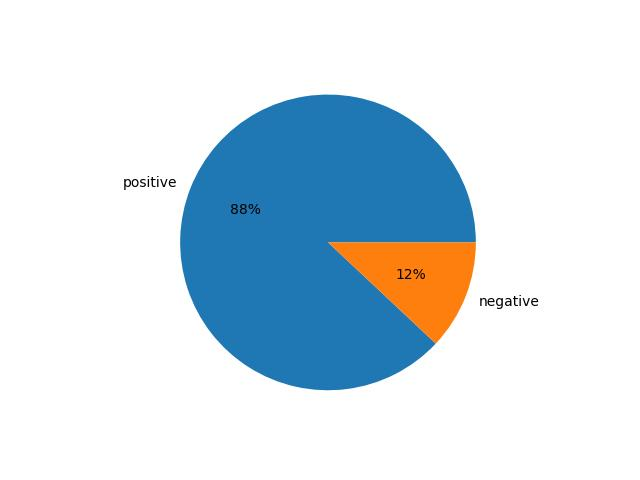
\includegraphics[width=7cm]{figuras/TripAdvisor/Hotels/hotel0_sentiments.jpeg}
\caption{Gráfico circular gerado baseando-se nos \textit{sentiments} mais usados da plataforma \textit{TripAdvisor} referente à Pousada Convento Beja}
\label{fig:exemplofig}
\end{figure}

\begin{figure}[!htb]
\centering
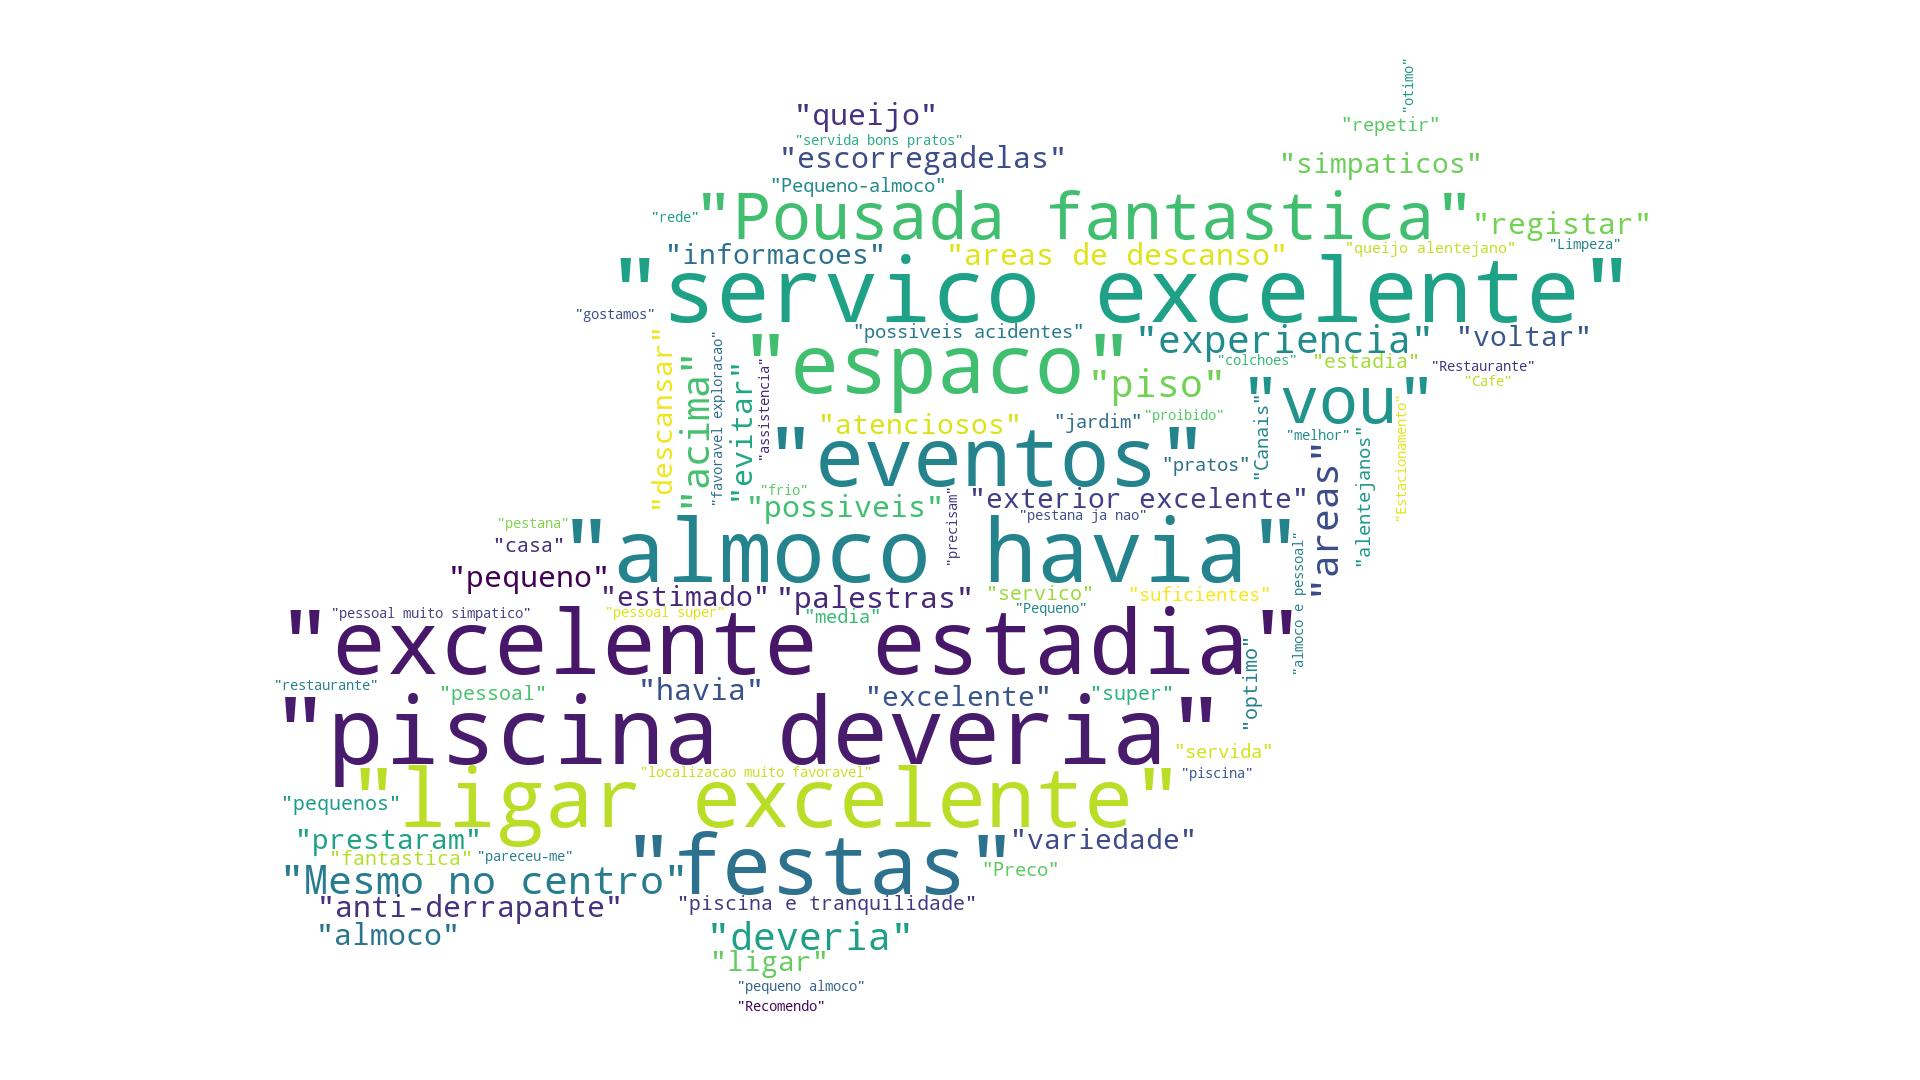
\includegraphics[width=7cm]{figuras/TripAdvisor/Hotels/hotel0_keywordcloud.jpeg}
\caption{Gráfico de palavras-chave e nuvens de palavras-chave contendo as \textit{keywords} mais usadas da plataforma \textit{TripAdvisor} referente à Pousada Convento Beja}
\label{fig:exemplofig}
\end{figure}

\begin{figure}[!htb]
\centering
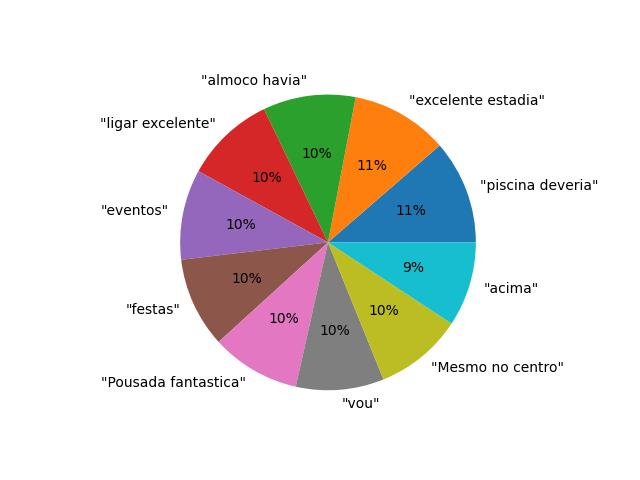
\includegraphics[width=7cm]{figuras/TripAdvisor/Hotels/hotel0_keywords.jpeg}
\caption{Gráfico circular gerado baseando-se nas \textit{keywords} mais usadas da plataforma \textit{TripAdvisor} referente à Pousada Convento Beja}
\label{fig:exemplofig}
\end{figure}

\begin{figure}[!htb]
\centering
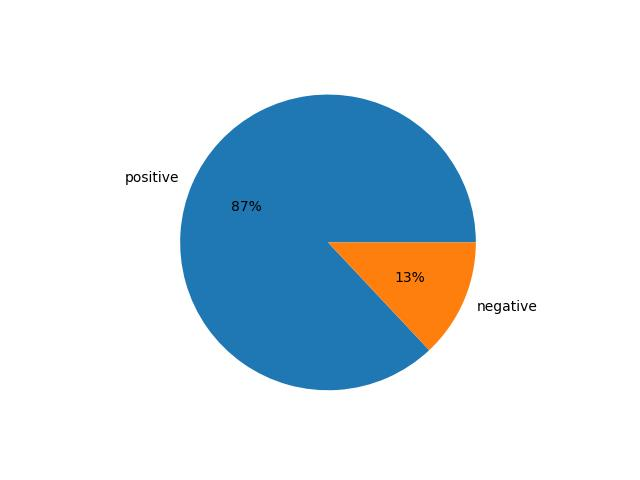
\includegraphics[width=7cm]{figuras/TripAdvisor/Hotels/hotel8_sentiments.jpeg}
\caption{Gráfico circular gerado baseando-se nos \textit{sentiments} mais usados da plataforma \textit{TripAdvisor} referente ao Hotel São Domingos}
\label{fig:exemplofig}
\end{figure}

\begin{figure}[!htb]
\centering
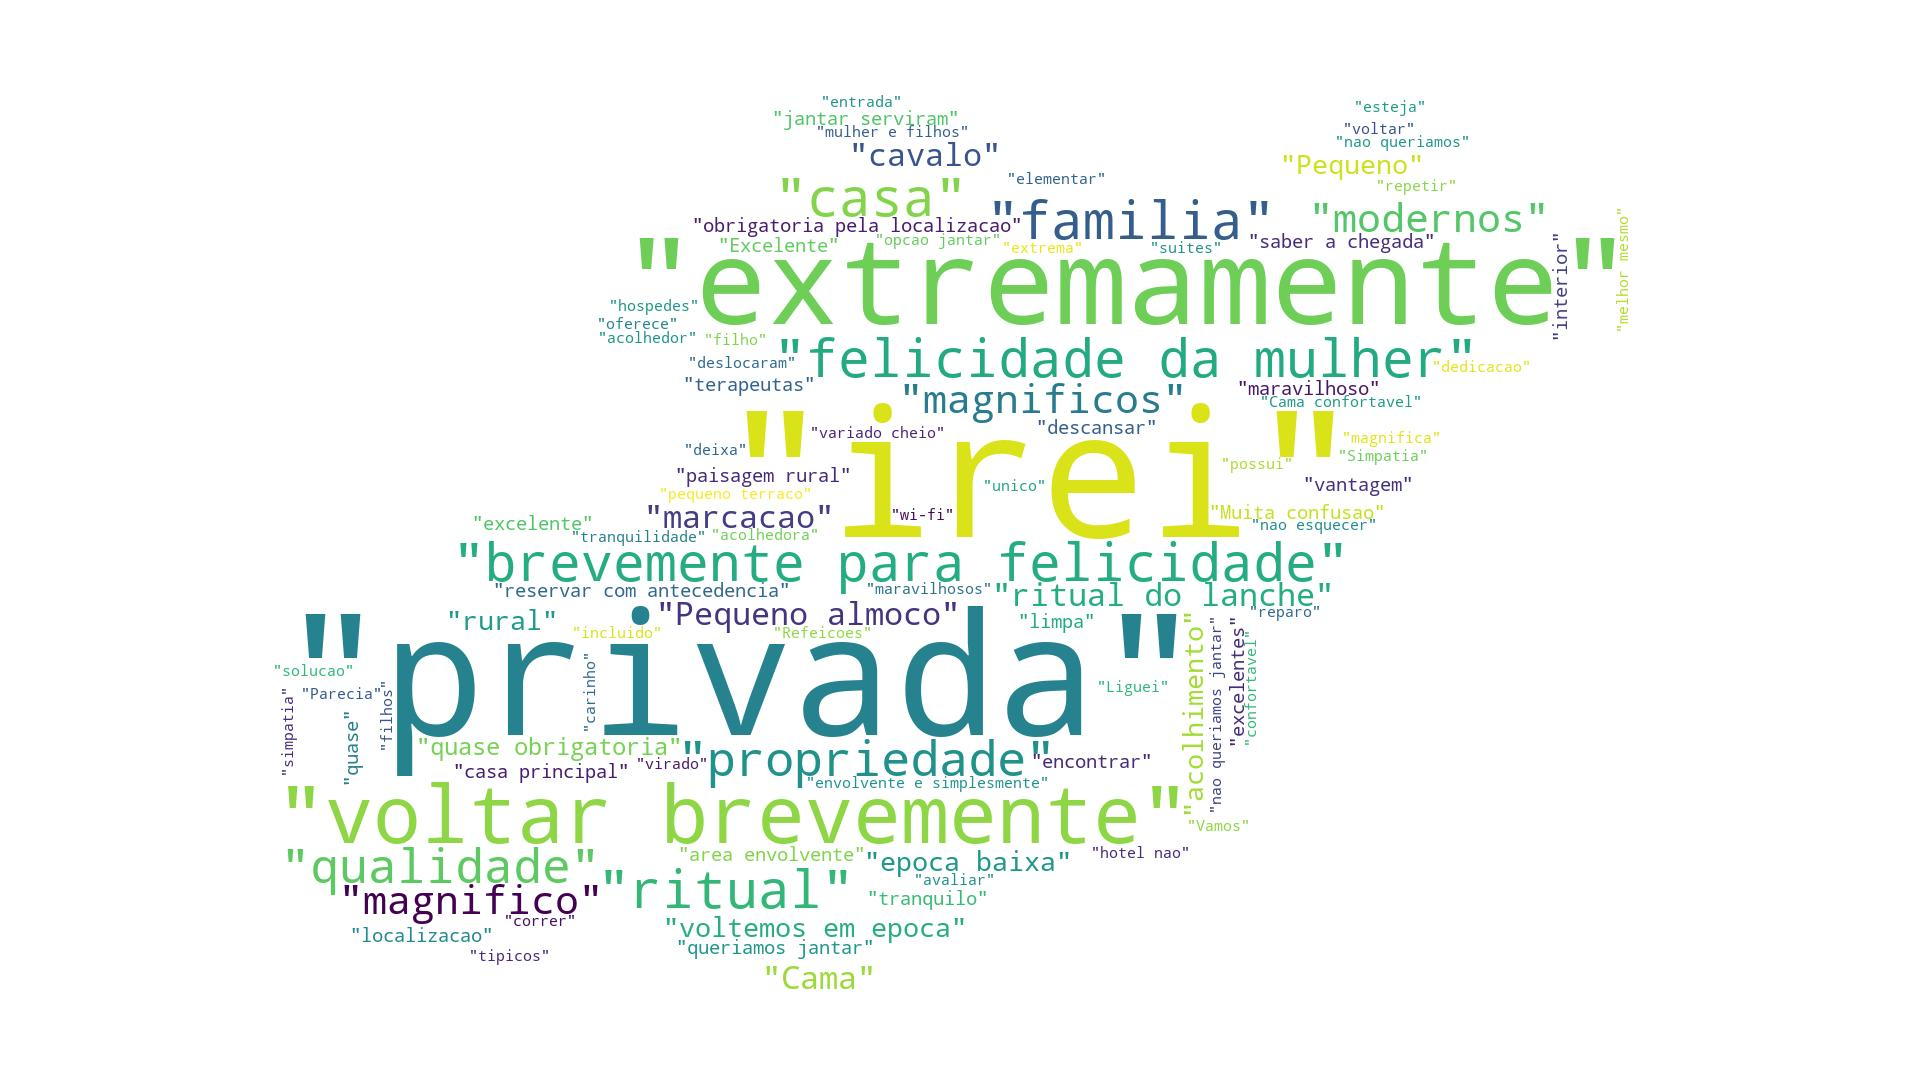
\includegraphics[width=7cm]{figuras/TripAdvisor/Hotels/hotel8_keywordcloud.jpeg}
\caption{Gráfico de palavras-chave e nuvens de palavras-chave contendo as \textit{keywords} mais usadas da plataforma \textit{TripAdvisor} referente ao Hotel São Domingos}
\label{fig:exemplofig}
\end{figure}

\begin{figure}[!htb]
\centering
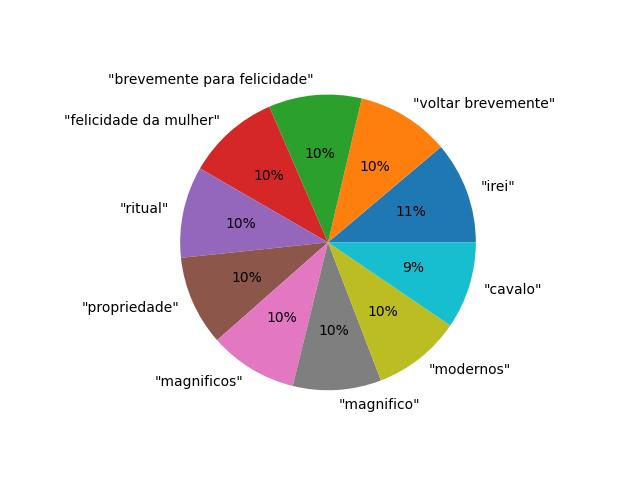
\includegraphics[width=7cm]{figuras/TripAdvisor/Hotels/hotel8_keywords.jpeg}
\caption{Gráfico circular gerado baseando-se nas \textit{keywords} mais usadas da plataforma \textit{TripAdvisor} referente ao Hotel São Domingos}
\label{fig:exemplofig}
\end{figure}

\begin{figure}[!htb]
\centering
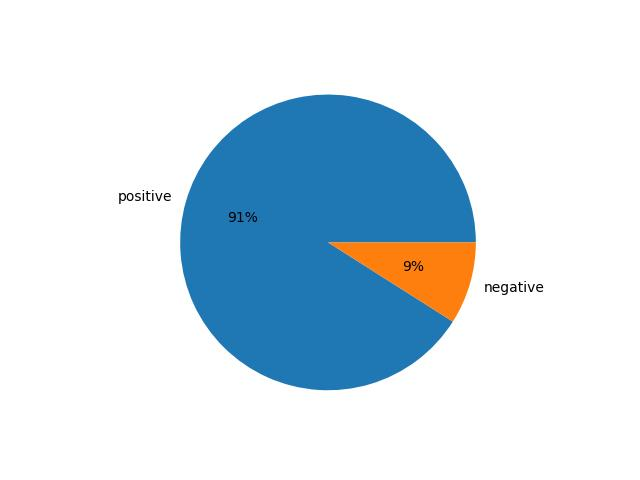
\includegraphics[width=7cm]{figuras/TripAdvisor/Hotels/hotel21_sentiments.jpeg}
\caption{Gráfico circular gerado baseando-se nos \textit{sentiments} mais usados da plataforma \textit{TripAdvisor} referente à Herdade das Barradas da Serra}
\label{fig:exemplofig}
\end{figure}

\begin{figure}[!htb]
\centering
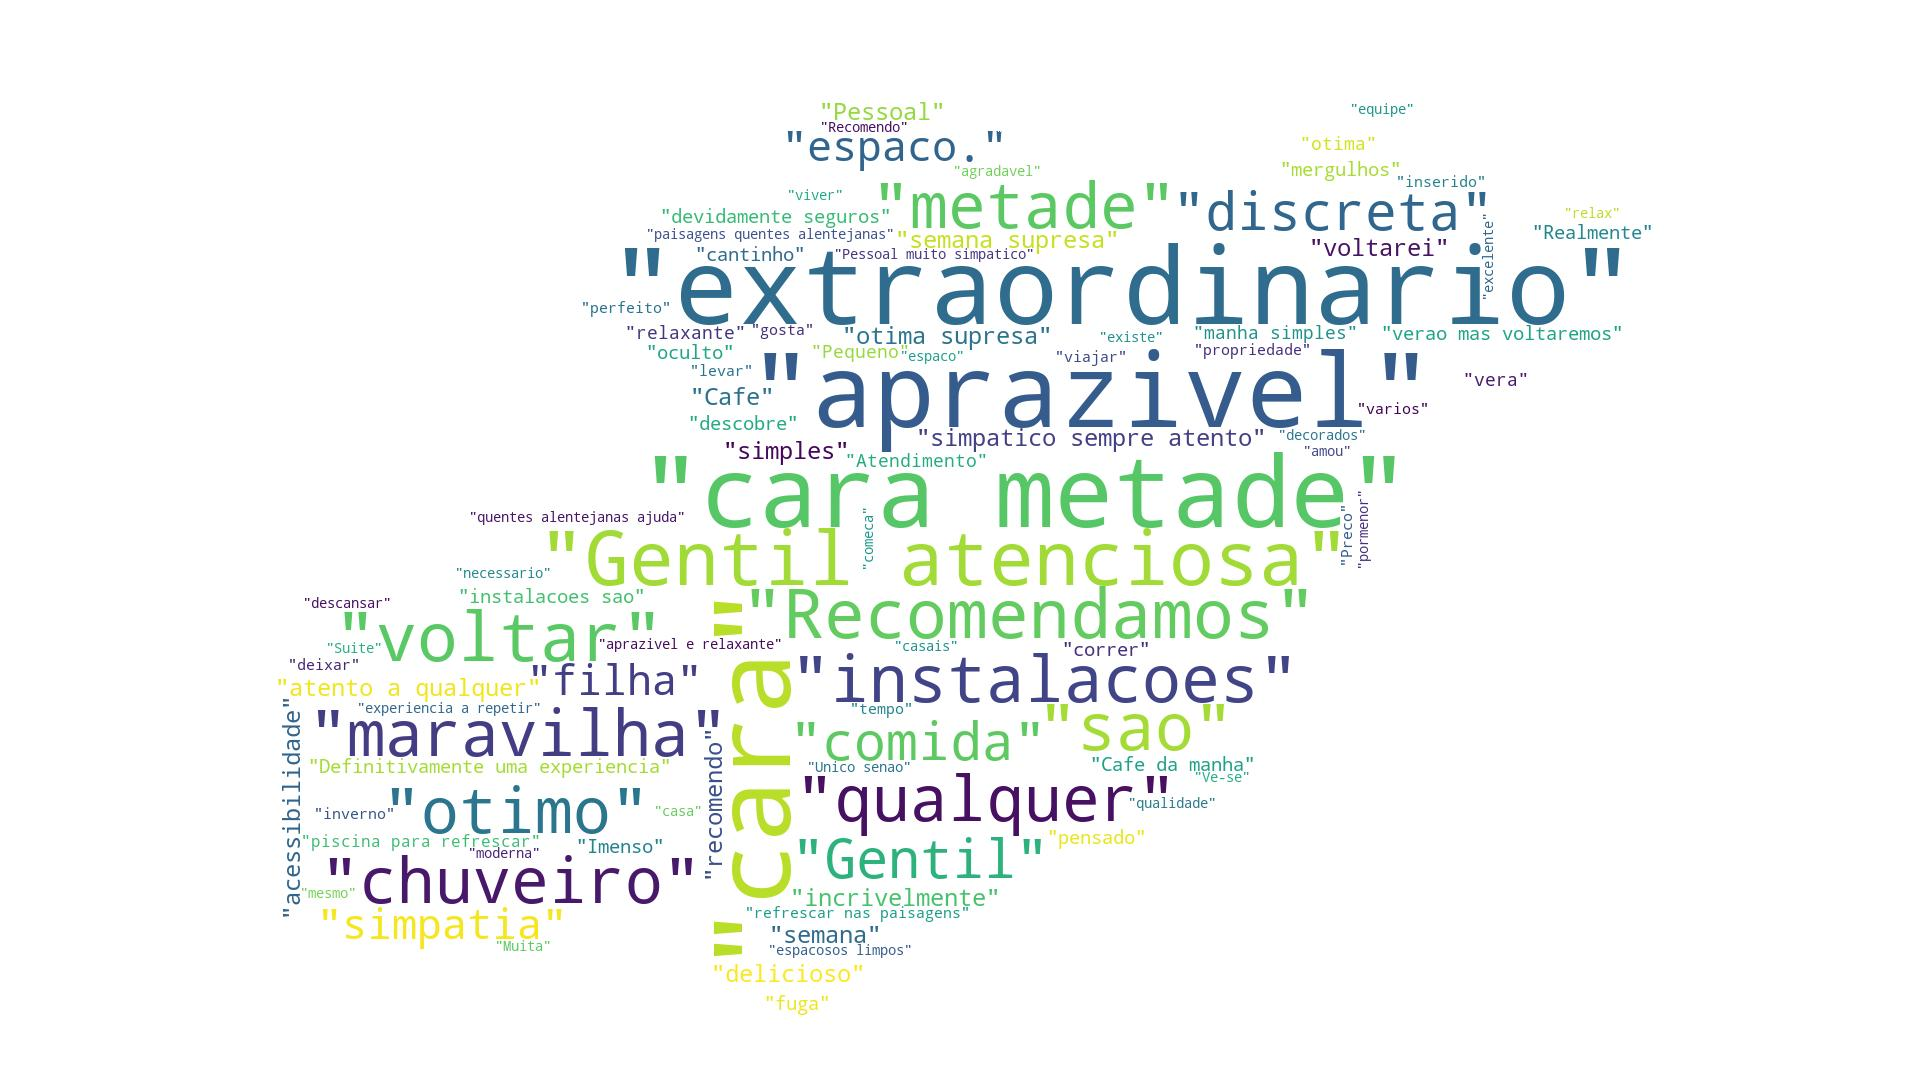
\includegraphics[width=7cm]{figuras/TripAdvisor/Hotels/hotel21_keywordcloud.jpeg}
\caption{Gráfico de palavras-chave e nuvens de palavras-chave contendo as \textit{keywords} mais usadas da plataforma \textit{TripAdvisor} referente à Herdade das Barradas da Serra}
\label{fig:exemplofig}
\end{figure}

\begin{figure}[!htb]
\centering
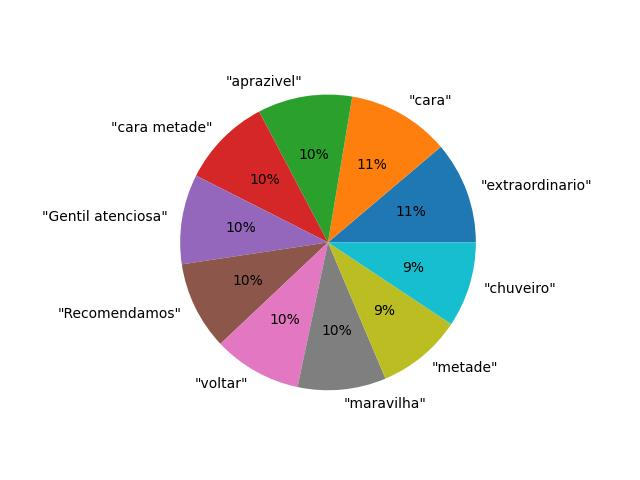
\includegraphics[width=7cm]{figuras/TripAdvisor/Hotels/hotel21_keywords.jpeg}
\caption{Gráfico circular gerado baseando-se nas \textit{keywords} mais usadas da plataforma \textit{TripAdvisor} referente à Herdade das Barradas da Serra}
\label{fig:exemplofig}
\end{figure}


\chapter{Anexo referente às imagens dos gráficos utilizados no relatório (Tripadvisor-Restaurantes)}

Acesso a todos os gráficos originados: \href{https://github.com/CatKinKitKat/pi2021/tree/master/projecto/datascience/graphs/tripadvisor/restaurants}{GitHub}.

\label{an1}
\begin{figure}[!htb]
\centering
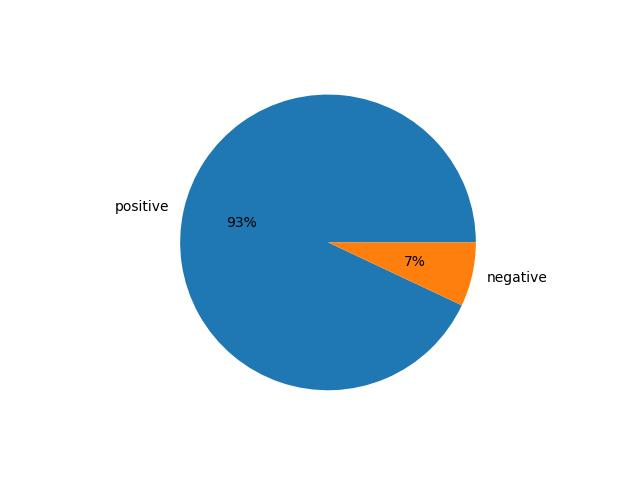
\includegraphics[width=7cm]{figuras/TripAdvisor/Restaurants/restaurant0_sentiments.jpeg}
\caption{Gráfico circular gerado baseando-se nos \textit{sentiments} mais usados da plataforma \textit{Tripadvisor} referente ao restaurante 0}
\label{fig:exemplofig}
\end{figure}

\begin{figure}[!htb]
\centering
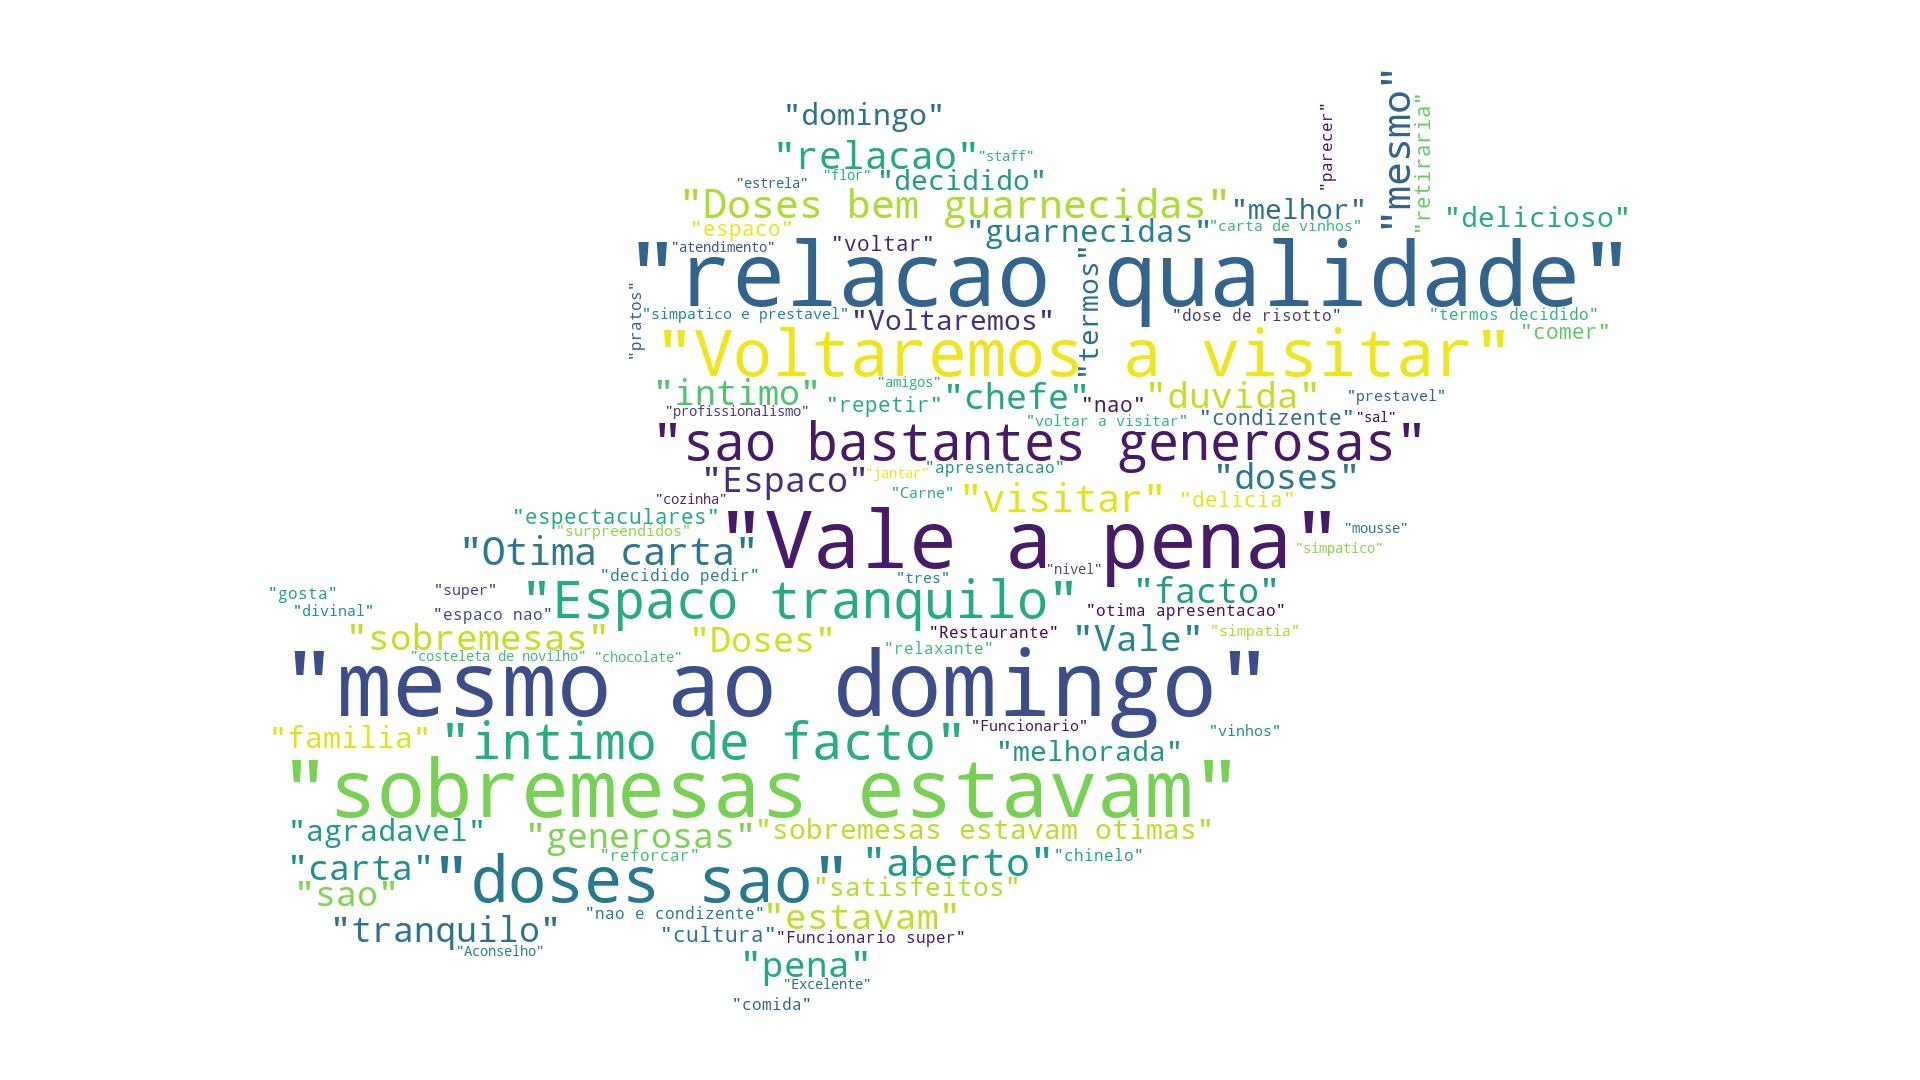
\includegraphics[width=7cm]{figuras/TripAdvisor/Restaurants/restaurant0_keywordcloud.jpeg}
\caption{Gráfico de palavras-chave e nuvens de palavras-chave contendo as \textit{keywords} mais usadas da plataforma \textit{Tripadvisor} referente ao restaurante 0}
\label{fig:exemplofig}
\end{figure}

\begin{figure}[!htb]
\centering
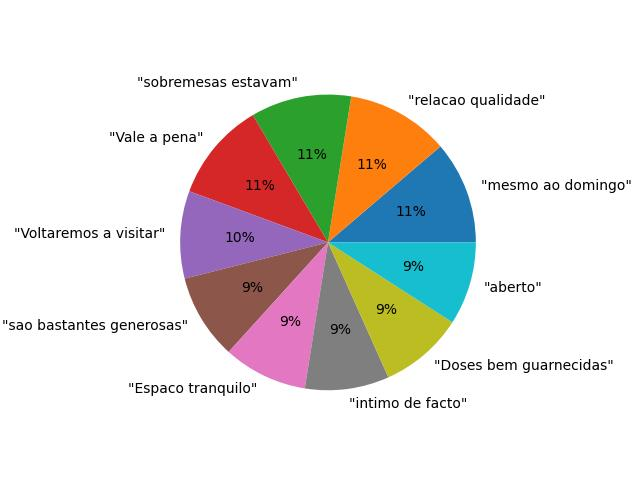
\includegraphics[width=7cm]{figuras/TripAdvisor/Restaurants/restaurant0_keywords.jpeg}
\caption{Gráfico circular gerado baseando-se nas \textit{keywords} mais usadas da plataforma \textit{Tripadvisor} referente ao restaurante 0}
\label{fig:exemplofig}
\end{figure}

\begin{figure}[!htb]
\centering
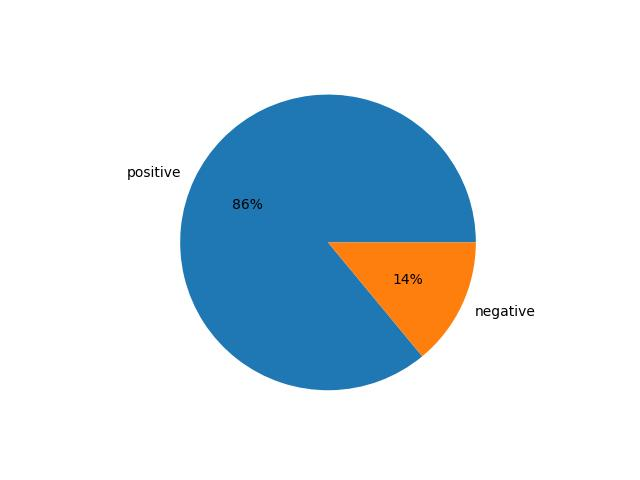
\includegraphics[width=7cm]{figuras/TripAdvisor/Restaurants/restaurant8_sentiments.jpeg}
\caption{Gráfico circular gerado baseando-se nos \textit{sentiments} mais usados da plataforma \textit{Tripadvisor} referente ao restaurante 8}
\label{fig:exemplofig}
\end{figure}

\begin{figure}[!htb]
\centering
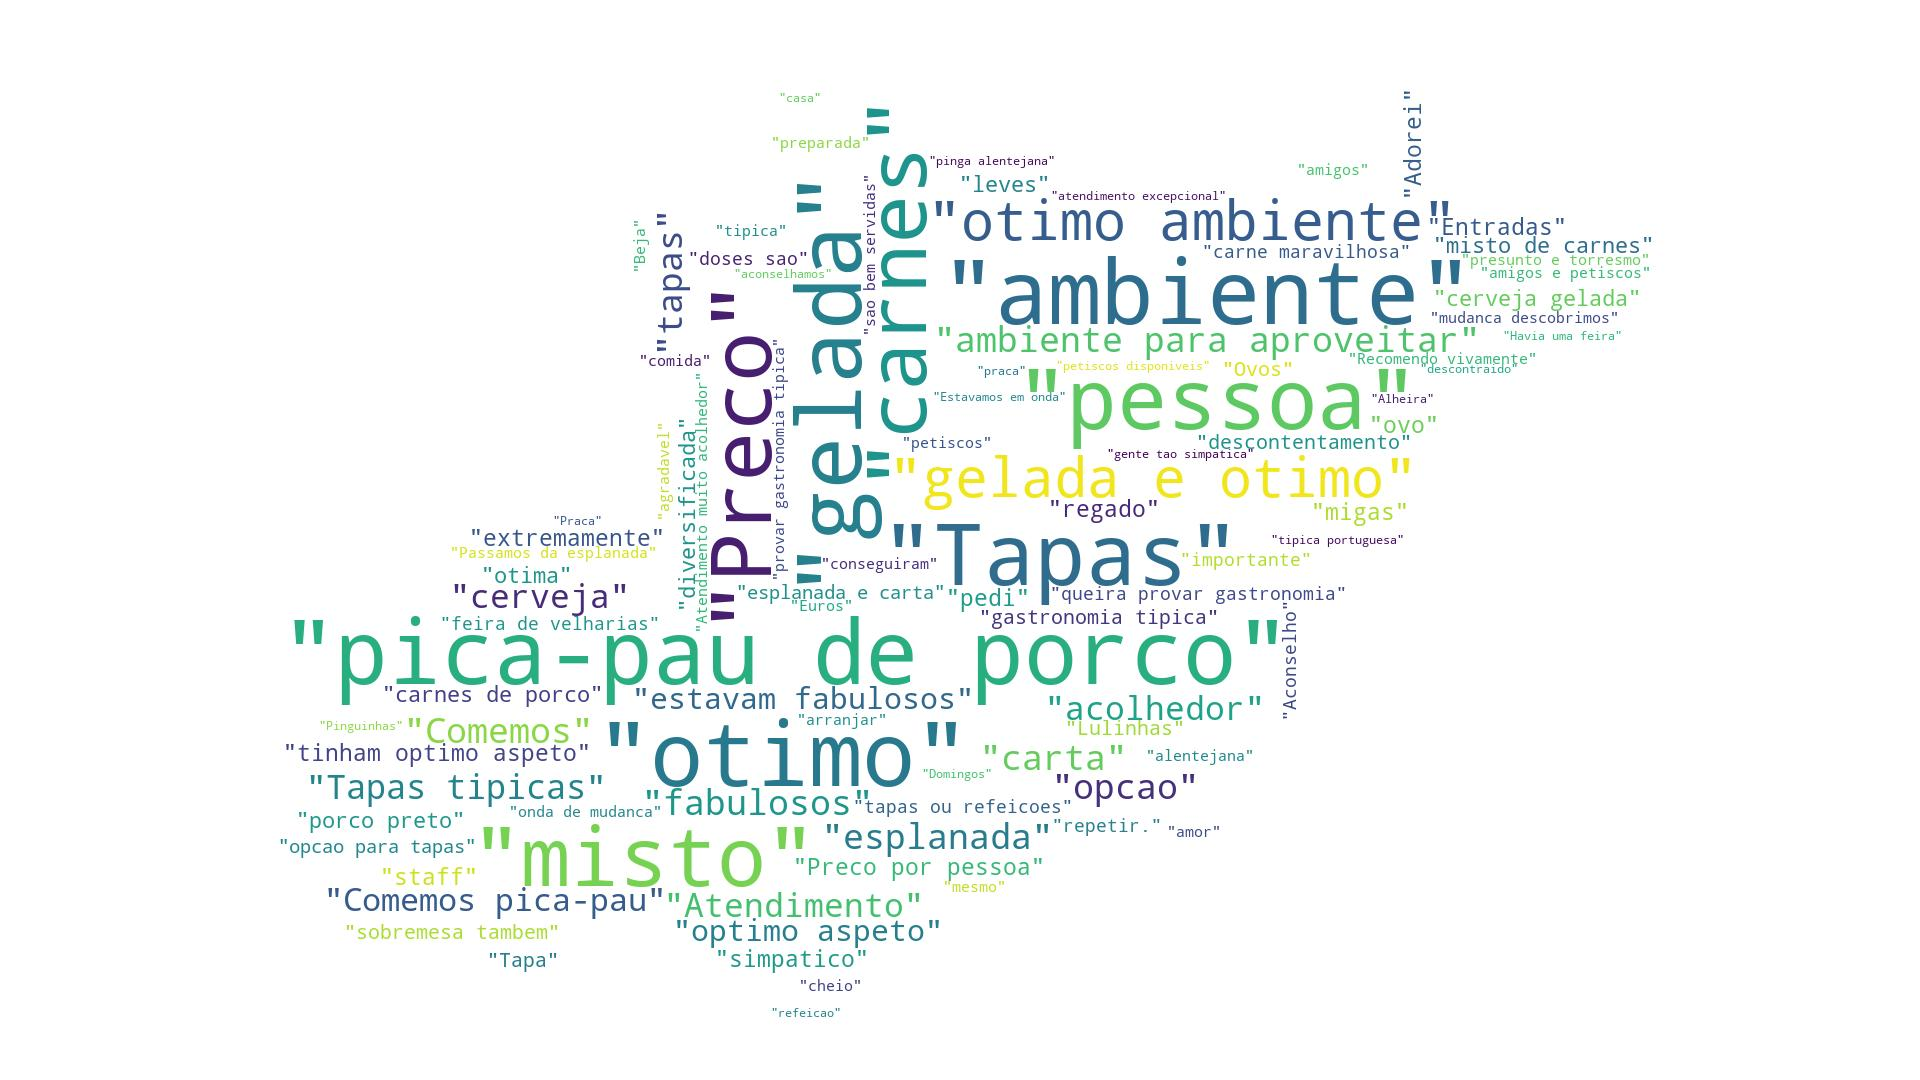
\includegraphics[width=7cm]{figuras/TripAdvisor/Restaurants/restaurant8_keywordcloud.jpeg}
\caption{Gráfico de palavras-chave e nuvens de palavras-chave contendo as \textit{keywords} mais usadas da plataforma \textit{Tripadvisor} referente ao restaurante 8}
\label{fig:exemplofig}
\end{figure}

\begin{figure}[!htb]
\centering
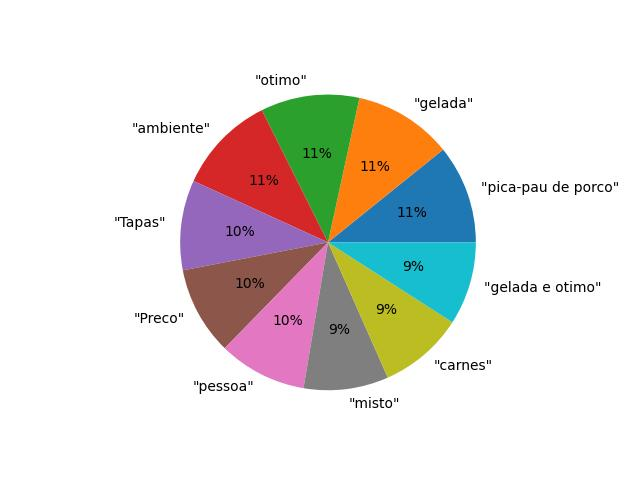
\includegraphics[width=7cm]{figuras/TripAdvisor/Restaurants/restaurant8_keywords.jpeg}
\caption{Gráfico circular gerado baseando-se nas \textit{keywords} mais usadas da plataforma \textit{Tripadvisor} referente ao restaurante 8}
\label{fig:exemplofig}
\end{figure}

\begin{figure}[!htb]
\centering
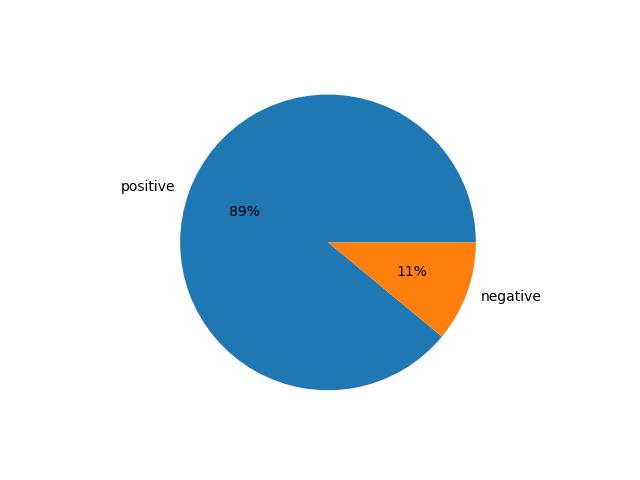
\includegraphics[width=7cm]{figuras/TripAdvisor/Restaurants/restaurant21_sentiments.jpeg}
\caption{Gráfico circular gerado baseando-se nos \textit{sentiments} mais usados da plataforma \textit{Tripadvisor} referente ao restaurante 21}
\label{fig:exemplofig}
\end{figure}

\begin{figure}[!htb]
\centering
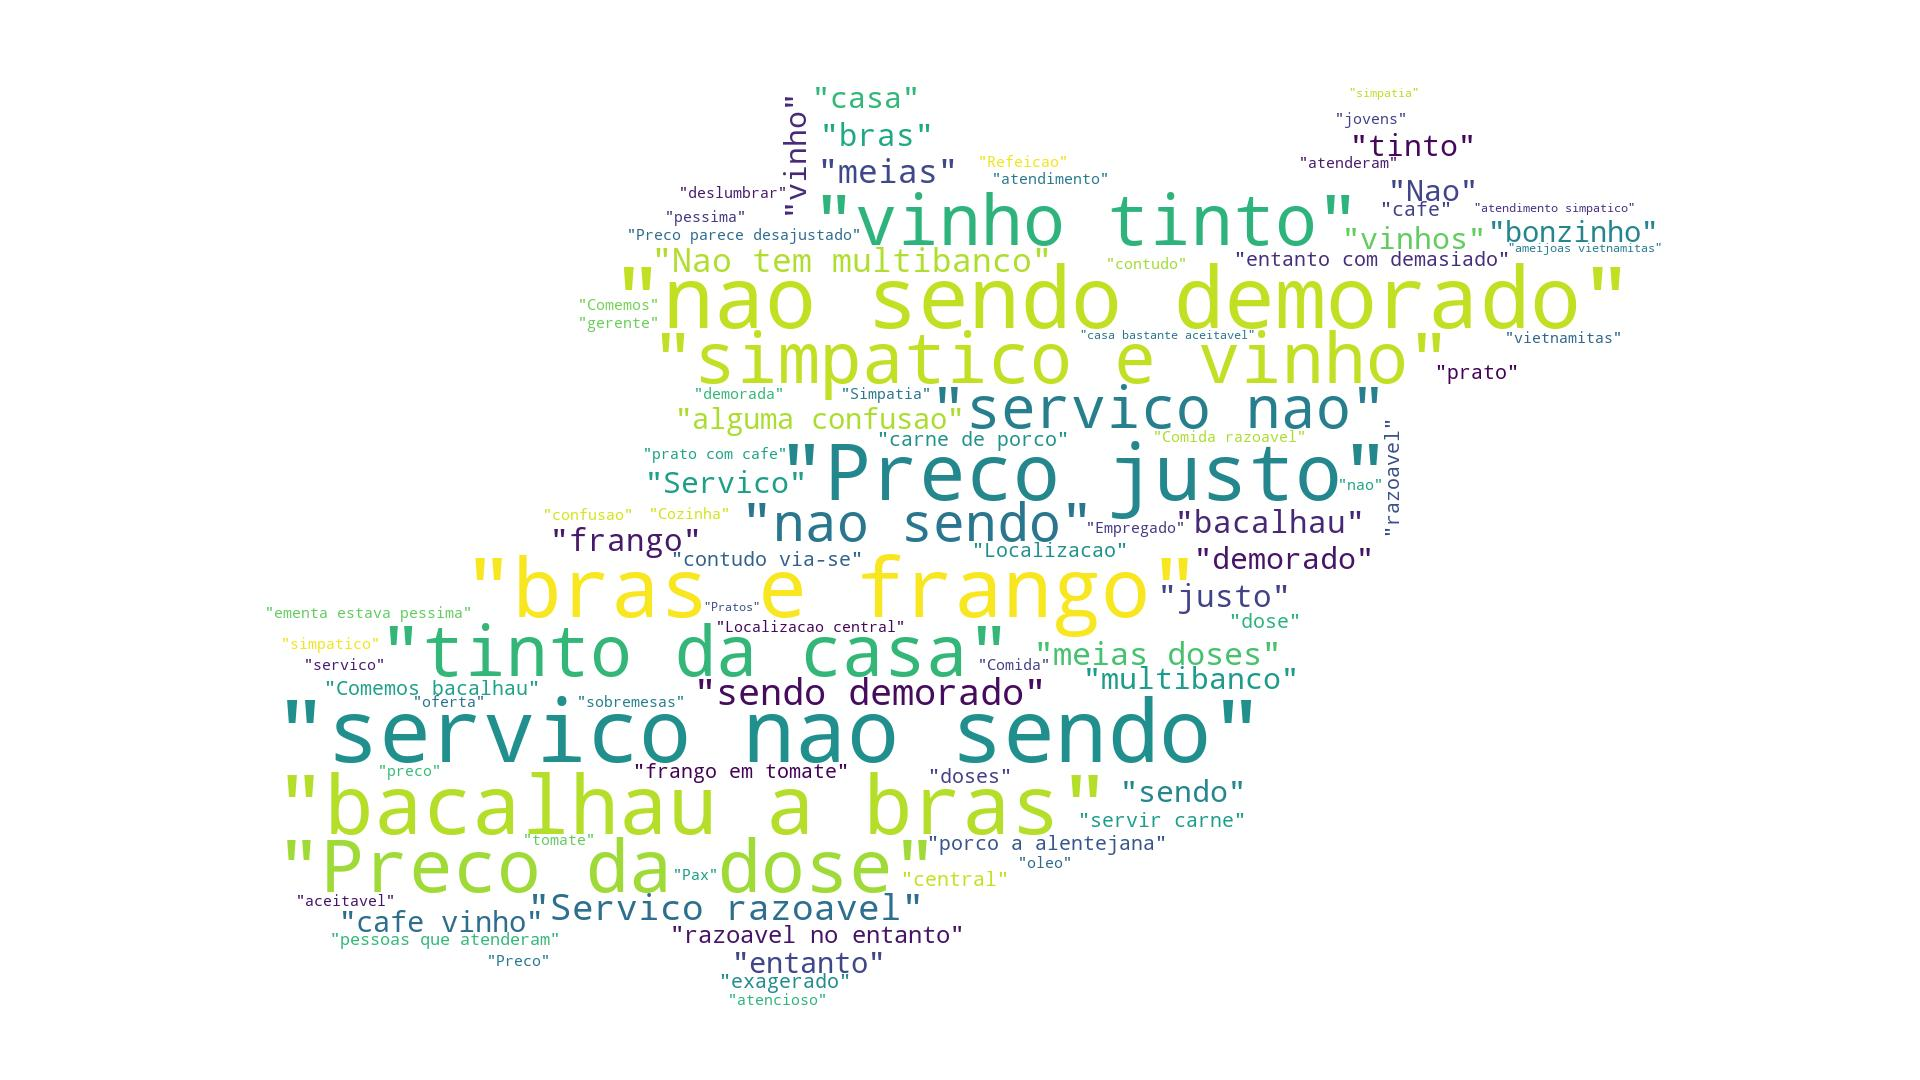
\includegraphics[width=7cm]{figuras/TripAdvisor/Restaurants/restaurant21_keywordcloud.jpeg}
\caption{Gráfico de palavras-chave e nuvens de palavras-chave contendo as \textit{keywords} mais usadas da plataforma \textit{Tripadvisor} referente ao restaurante 21}
\label{fig:exemplofig}
\end{figure}

\begin{figure}[!htb]
\centering
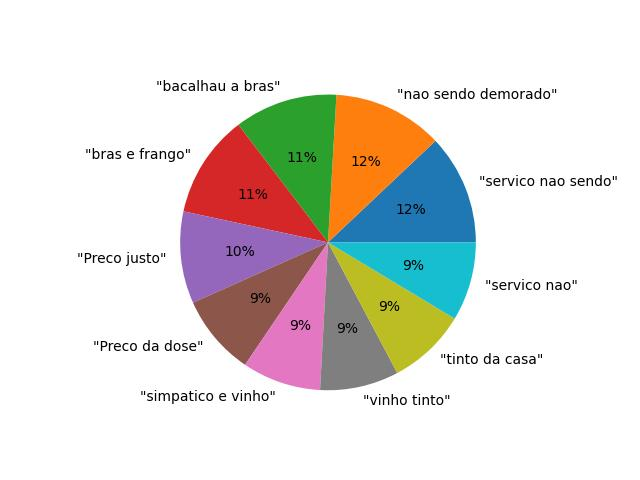
\includegraphics[width=7cm]{figuras/TripAdvisor/Restaurants/restaurant21_keywords.jpeg}
\caption{Gráfico circular gerado baseando-se nas \textit{keywords} mais usadas da plataforma \textit{Tripadvisor} referente ao restaurante 21}
\label{fig:exemplofig}
\end{figure}


    \chapter{Anexo referente às imagens dos gráficos utilizados no relatório (TripAdvisor-Actividades)}
    
    Acesso a todos os gráficos originados: \href{https://github.com/CatKinKitKat/pi2021/tree/master/projecto/datascience/graphs/TripAdvisor/activities}{GitHub}.
    
    \label{an3}
    \begin{figure}[!htb]
    \centering
    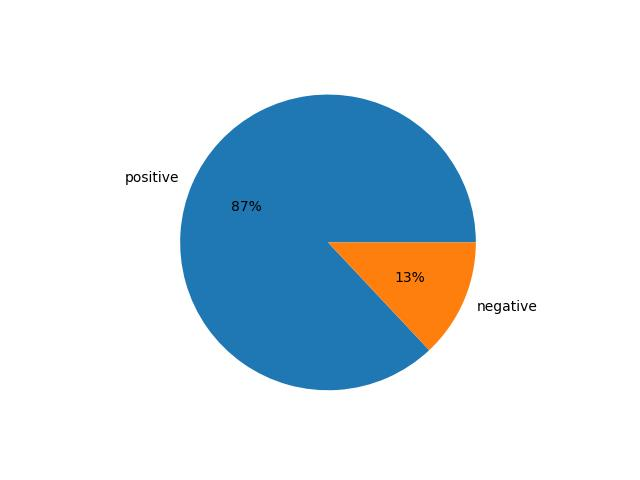
\includegraphics[width=7cm]{figuras/TripAdvisor/Activities/place0_sentiments.jpeg}
    \caption{Gráfico circular gerado baseando-se nos \textit{sentiments} mais usados da plataforma \textit{TripAdvisor} referente ao Castelo de Beja}
    \label{fig:exemplofig}
    \end{figure}
    
    \begin{figure}[!htb]
    \centering
    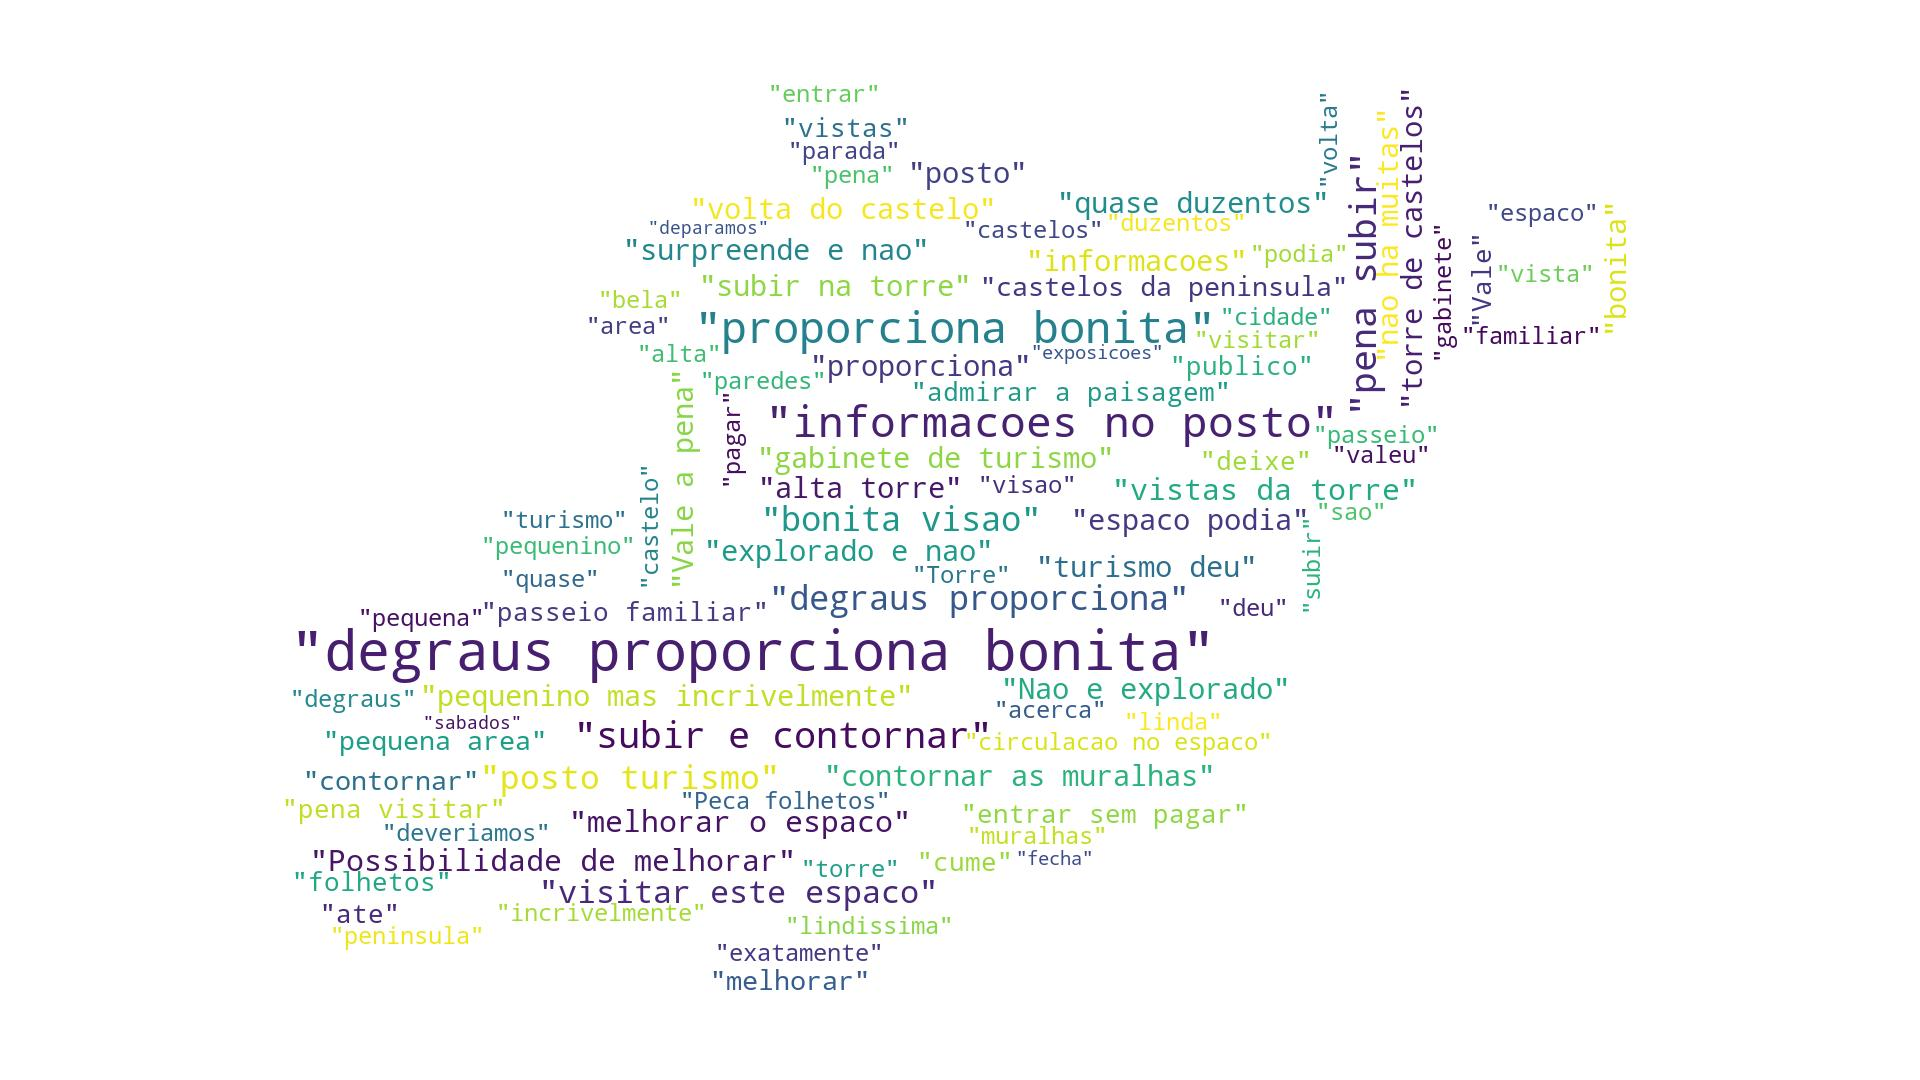
\includegraphics[width=7cm]{figuras/TripAdvisor/Activities/place0_keywordcloud.jpeg}
    \caption{Gráfico de palavras-chave e nuvens de palavras-chave contendo as \textit{keywords} mais usadas da plataforma \textit{TripAdvisor} referente ao Castelo de Beja}
    \label{fig:exemplofig}
    \end{figure}
    
    \begin{figure}[!htb]
    \centering
    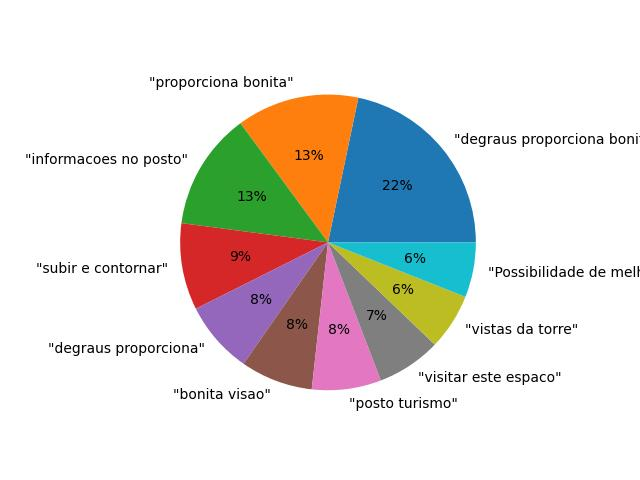
\includegraphics[width=7cm]{figuras/TripAdvisor/Activities/place0_keywords.jpeg}
    \caption{Gráfico circular gerado baseando-se nas \textit{keywords} mais usadas da plataforma \textit{TripAdvisor} referente ao Castelo de Beja}
    \label{fig:exemplofig}
    \end{figure}
    
    \begin{figure}[!htb]
    \centering
    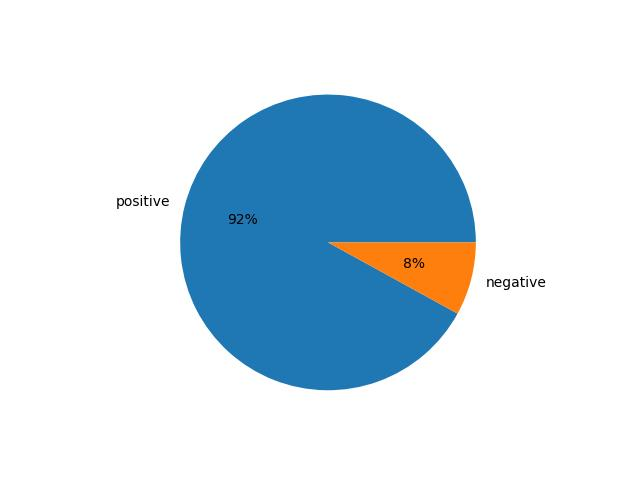
\includegraphics[width=7cm]{figuras/TripAdvisor/Activities/place8_sentiments.jpeg}
    \caption{Gráfico circular gerado baseando-se nos \textit{sentiments} mais usados da plataforma \textit{TripAdvisor} referente à Catedral de Beja}
    \label{fig:exemplofig}
    \end{figure}
    
    \begin{figure}[!htb]
    \centering
    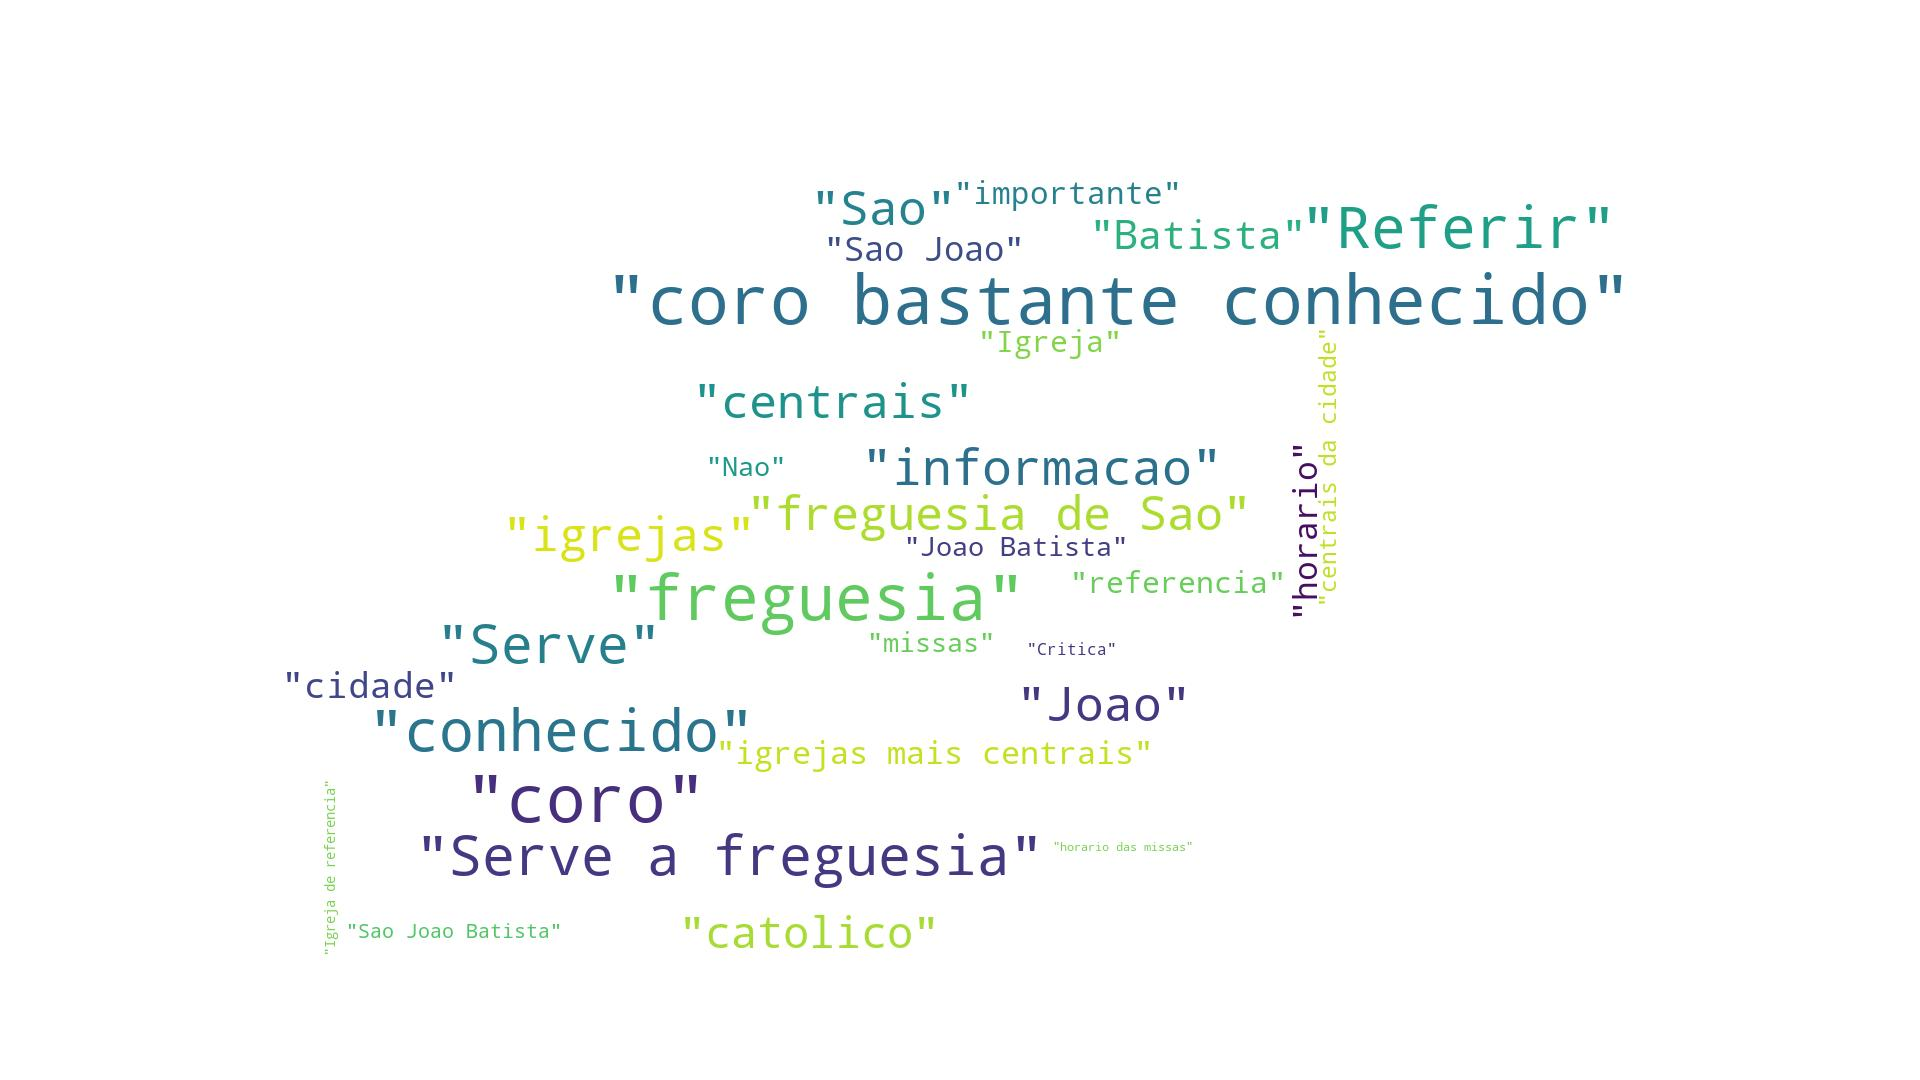
\includegraphics[width=7cm]{figuras/TripAdvisor/Activities/place8_keywordcloud.jpeg}
    \caption{Gráfico de palavras-chave e nuvens de palavras-chave contendo as \textit{keywords} mais usadas da plataforma \textit{TripAdvisor} referente à Catedral de Beja}
    \label{fig:exemplofig}
    \end{figure}
    
    \begin{figure}[!htb]
    \centering
    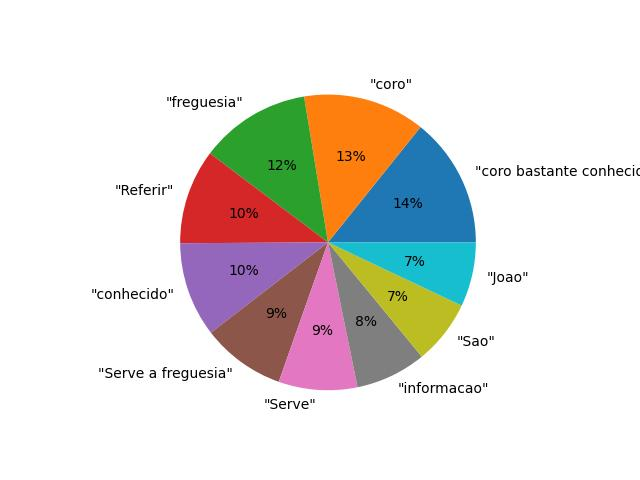
\includegraphics[width=7cm]{figuras/TripAdvisor/Activities/place8_keywords.jpeg}
    \caption{Gráfico circular gerado baseando-se nas \textit{keywords} mais usadas da plataforma \textit{TripAdvisor} referente à Catedral de Beja}
    \label{fig:exemplofig}
    \end{figure}
    
    \begin{figure}[!htb]
    \centering
    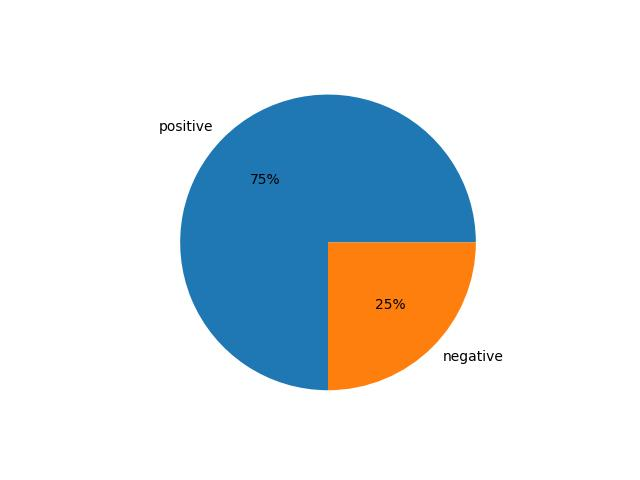
\includegraphics[width=7cm]{figuras/TripAdvisor/Activities/place21_sentiments.jpeg}
    \caption{Gráfico circular gerado baseando-se nos \textit{sentiments} mais usados da plataforma \textit{TripAdvisor} referente à Janela Manuelina}
    \label{fig:exemplofig}
    \end{figure}
    
    \begin{figure}[!htb]
    \centering
    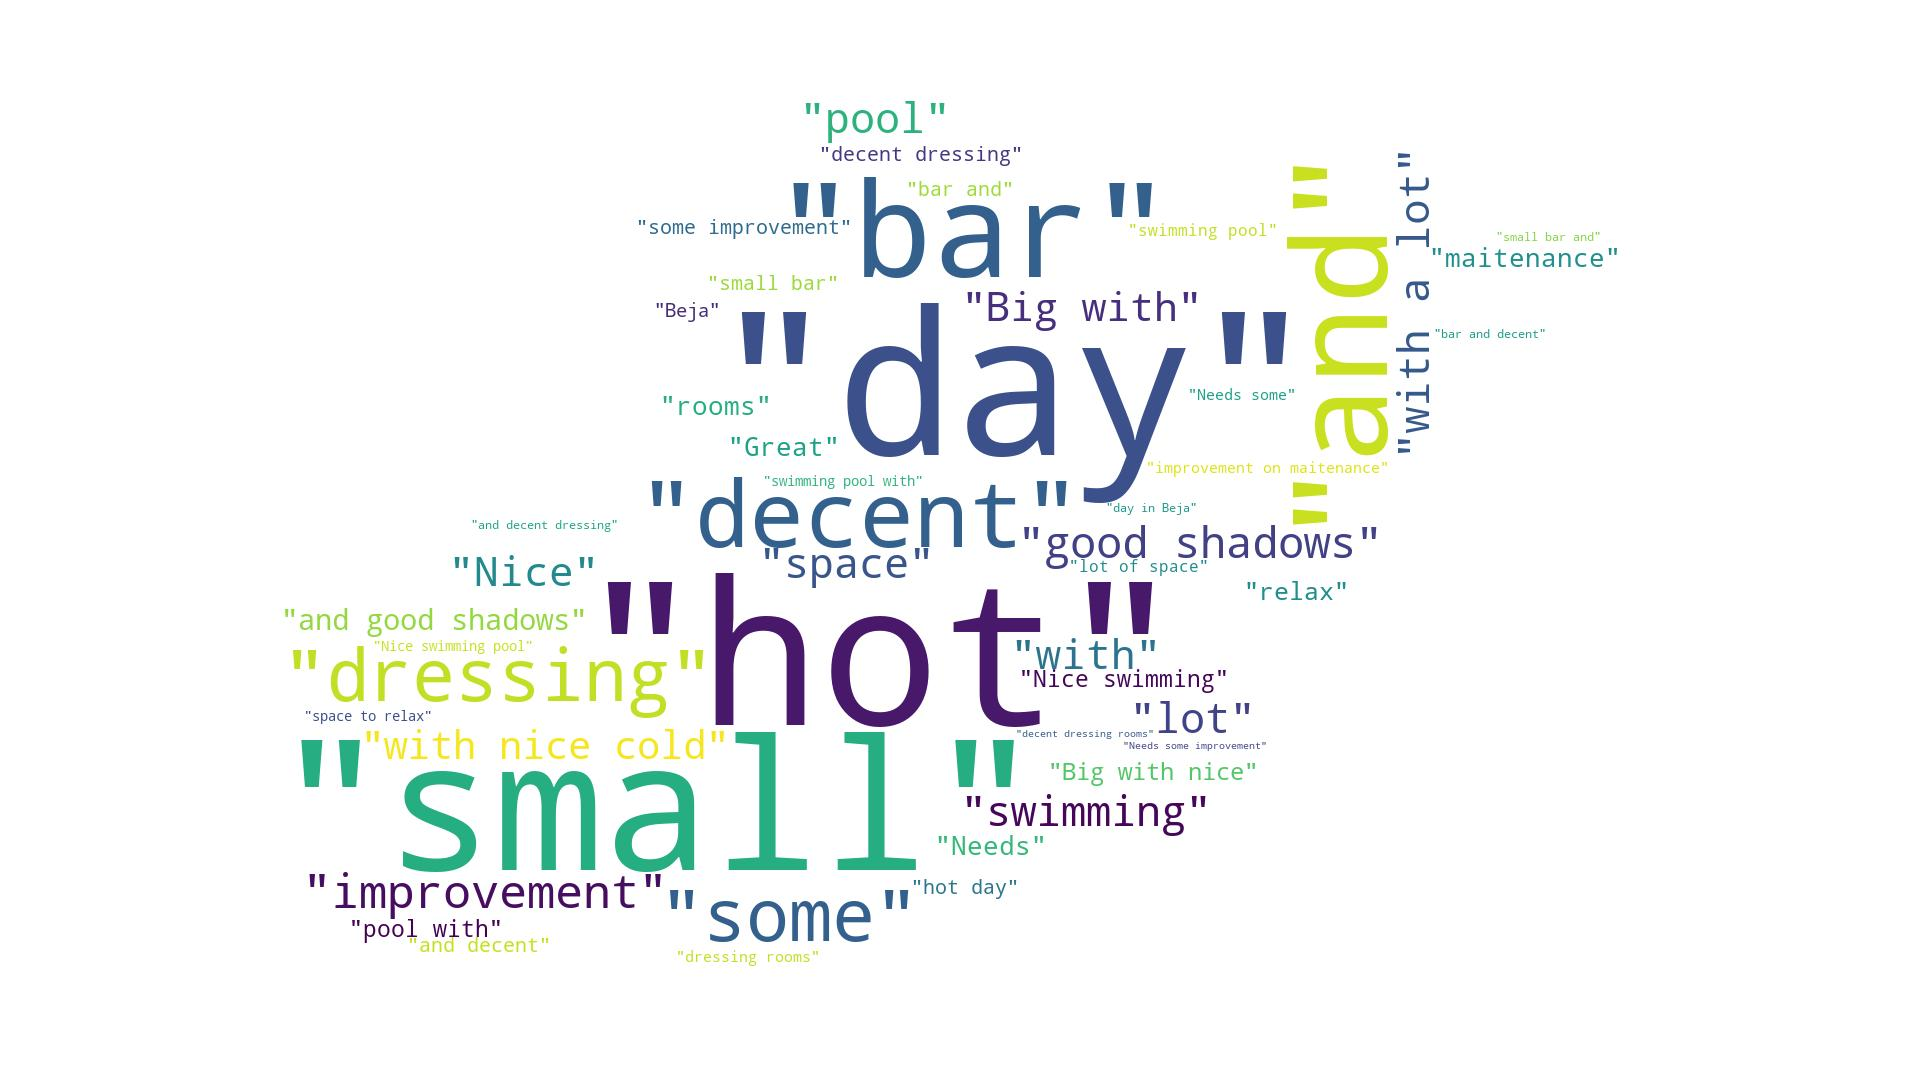
\includegraphics[width=7cm]{figuras/TripAdvisor/Activities/place21_keywordcloud.jpeg}
    \caption{Gráfico de palavras-chave e nuvens de palavras-chave contendo as \textit{keywords} mais usadas da plataforma \textit{TripAdvisor} referente à Janela Manuelina}
    \label{fig:exemplofig}
    \end{figure}
    
    \begin{figure}[!htb]
    \centering
    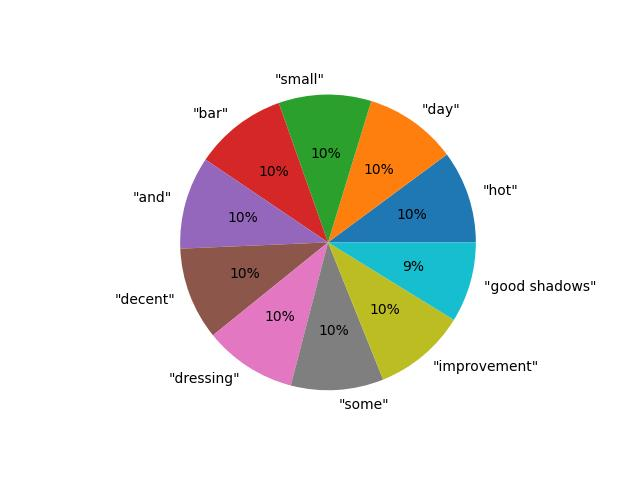
\includegraphics[width=7cm]{figuras/TripAdvisor/Activities/place21_keywords.jpeg}
    \caption{Gráfico circular gerado baseando-se nas \textit{keywords} mais usadas da plataforma \textit{TripAdvisor} referente à Janela Manuelina}
    \label{fig:exemplofig}
    \end{figure}
    

\chapter{Anexo referente às imagens dos gráficos utilizados no relatório (Booking)}

Acesso a todos os gráficos originados: \href{https://github.com/CatKinKitKat/pi2021/tree/master/projecto/datascience/graphs/booking/hotels}{GitHub}.

\label{an1}
\begin{figure}[!htb]
\centering
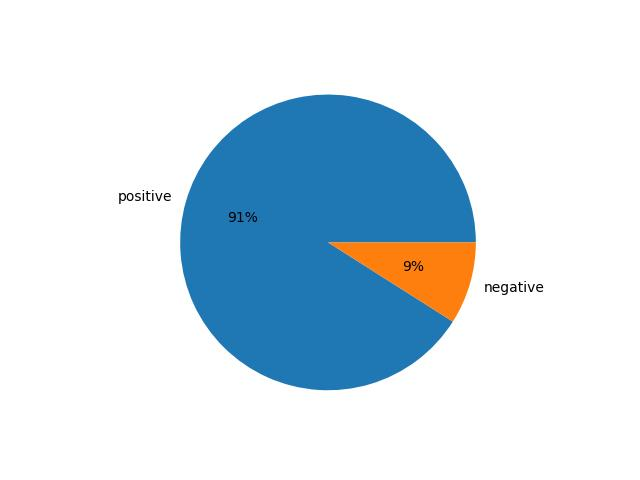
\includegraphics[width=7cm]{figuras/Booking/hotel1_sentiments.jpeg}
\caption{Gráfico circular gerado baseando-se nos \textit{sentiments} mais usados da plataforma \textit{Booking} referente ao hótel 1}
\label{fig:exemplofig}
\end{figure}

\begin{figure}[!htb]
\centering
\includegraphics[width=7cm]{figuras/Booking/hotel1_keywordcloud.jpeg}
\caption{Gráfico de palavras-chave e nuvens de palavras-chave contendo as \textit{keywords} mais usadas da plataforma \textit{Booking} referente ao hótel 1}
\label{fig:exemplofig}
\end{figure}

\begin{figure}[!htb]
\centering
\includegraphics[width=7cm]{figuras/Booking/hotel1_keywords.jpeg}
\caption{Gráfico circular gerado baseando-se nas \textit{keywords} mais usadas da plataforma \textit{Booking} referente ao hótel 1}
\label{fig:exemplofig}
\end{figure}

\begin{figure}[!htb]
\centering
\includegraphics[width=7cm]{figuras/Booking/hotel5_sentiments.jpeg}
\caption{Gráfico circular gerado baseando-se nos \textit{sentiments} mais usados da plataforma \textit{Booking} referente ao hótel 5}
\label{fig:exemplofig}
\end{figure}

\begin{figure}[!htb]
\centering
\includegraphics[width=7cm]{figuras/Booking/hotel5_keywordcloud.jpeg}
\caption{Gráfico de palavras-chave e nuvens de palavras-chave contendo as \textit{keywords} mais usadas da plataforma \textit{Booking} referente ao hótel 5}
\label{fig:exemplofig}
\end{figure}

\begin{figure}[!htb]
\centering
\includegraphics[width=7cm]{figuras/Booking/hotel5_keywords.jpeg}
\caption{Gráfico circular gerado baseando-se nas \textit{keywords} mais usadas da plataforma \textit{Booking} referente ao hótel 5}
\label{fig:exemplofig}
\end{figure}

\begin{figure}[!htb]
\centering
\includegraphics[width=7cm]{figuras/Booking/hotel21_sentiments.jpeg}
\caption{Gráfico circular gerado baseando-se nos \textit{sentiments} mais usados da plataforma \textit{Booking} referente ao hótel 21}
\label{fig:exemplofig}
\end{figure}

\begin{figure}[!htb]
\centering
\includegraphics[width=7cm]{figuras/Booking/hotel21_keywordcloud.jpeg}
\caption{Gráfico de palavras-chave e nuvens de palavras-chave contendo as \textit{keywords} mais usadas da plataforma \textit{Booking} referente ao hótel 21}
\label{fig:exemplofig}
\end{figure}

\begin{figure}[!htb]
\centering
\includegraphics[width=7cm]{figuras/Booking/hotel21_keywords.jpeg}
\caption{Gráfico circular gerado baseando-se nas \textit{keywords} mais usadas da plataforma \textit{Booking} referente ao hótel 21}
\label{fig:exemplofig}
\end{figure}


\chapter{Anexo referente às imagens dos gráficos utilizados no relatório (Zomato)}
\label{an5}

Acesso a todos os gráficos originados: \href{https://github.com/CatKinKitKat/pi2021/tree/master/projecto/datascience/graphs/zomato/restaurantes}{GitHub}.

\begin{figure}[!htb]
\centering
\includegraphics[width=7cm]{figuras/Zomato/Restaurants/restaurante0_sentiments.jpeg}
\caption{Gráfico circular gerado baseando-se nos \textit{sentiments} mais usados da plataforma \textit{Zomato} referente ao restaurante Adega Típica 25 de Abril}
\label{fig:exemplofig}
\end{figure}

\begin{figure}[!htb]
\centering
\includegraphics[width=7cm]{figuras/Zomato/Restaurants/restaurante0_keywordcloud.jpeg}
\caption{Gráfico de palavras-chave e nuvens de palavras-chave contendo as \textit{keywords} mais usadas da plataforma \textit{Zomato} referente ao restaurante Adega Típica 25 de Abril}
\label{fig:exemplofig}
\end{figure}

\begin{figure}[!htb]
\centering
\includegraphics[width=7cm]{figuras/Zomato/Restaurants/restaurante0_keywords.jpeg}
\caption{Gráfico circular gerado baseando-se nas \textit{keywords} mais usadas da plataforma \textit{Zomato} referente ao restaurante Adega Típica 25 de Abril}
\label{fig:exemplofig}
\end{figure}

\begin{figure}[!htb]
\centering
\includegraphics[width=7cm]{figuras/Zomato/Restaurants/restaurante2_sentiments.jpeg}
\caption{Gráfico circular gerado baseando-se nos \textit{sentiments} mais usados da plataforma \textit{Zomato} referente ao restaurante Sushi Alentejano}
\label{fig:exemplofig}
\end{figure}

\begin{figure}[!htb]
\centering
\includegraphics[width=7cm]{figuras/Zomato/Restaurants/restaurante2_keywordcloud.jpeg}
\caption{Gráfico de palavras-chave e nuvens de palavras-chave contendo as \textit{keywords} mais usadas da plataforma \textit{Zomato} referente ao restaurante Sushi Alentejano}
\label{fig:exemplofig}
\end{figure}

\begin{figure}[!htb]
\centering
\includegraphics[width=7cm]{figuras/Zomato/Restaurants/restaurante2_keywords.jpeg}
\caption{Gráfico circular gerado baseando-se nas \textit{keywords} mais usadas da plataforma \textit{Zomato} referente ao restaurante Sushi Alentejano}
\label{fig:exemplofig}
\end{figure}

\begin{figure}[!htb]
\centering
\includegraphics[width=7cm]{figuras/Zomato/Restaurants/restaurante12_sentiments.jpeg}
\caption{Gráfico circular gerado baseando-se nos \textit{sentiments} mais usados da plataforma \textit{Zomato} referente ao restaurante Gatus Cervejaria Alentejana}
\label{fig:exemplofig}
\end{figure}

\begin{figure}[!htb]
\centering
\includegraphics[width=7cm]{figuras/Zomato/Restaurants/restaurante12_keywordcloud.jpeg}
\caption{Gráfico de palavras-chave e nuvens de palavras-chave contendo as \textit{keywords} mais usadas da plataforma \textit{Zomato} referente ao restaurante Gatus Cervejaria Alentejana}
\label{fig:exemplofig}
\end{figure}

\begin{figure}[!htb]
\centering
\includegraphics[width=7cm]{figuras/Zomato/Restaurants/restaurante12_keywords.jpeg}
\caption{Gráfico circular gerado baseando-se nas \textit{keywords} mais usadas da plataforma \textit{Zomato} referente ao restaurante Gatus Cervejaria Alentejana}
\label{fig:exemplofig}
\end{figure}


\chapter{Anexo referente às imagens dos gráficos utilizados no relatório (Tripadvisor - gráficos temporais)}

Acesso aos ficheiros \textit{PowerBI} criados e as imagens retiradas do mesmo:

\begin{enumerate}
    \item \href{https://github.com/CatKinKitKat/pi2021/blob/master/projecto/sql/Graphs.pbix}{GitHub gráficos PowerBI 1}.
    \item \href{https://github.com/CatKinKitKat/pi2021/blob/master/projecto/sql/qq.pbix}{GitHub gráficos PowerBI 2}.
    \item \href{https://github.com/CatKinKitKat/pi2021/tree/master/projecto/sql/screenshotsPowerBI}{GitHub PowerBI screenshots}.
\end{enumerate}

\label{an1}
\begin{figure}[!htb]
\centering
\includegraphics[width=7cm]{figuras/NegPerYear/4.PNG}
\caption{Gráfico de barras gerado baseando-se nos \textit{sentiments} mais usados da plataforma \textit{Tripadvisor} com níveis temporais sobre os \textit{sentiments} negativos ao longo do tempo}
\label{fig:exemplofig}
\end{figure}

\begin{figure}[!htb]
\centering
\includegraphics[width=7cm]{figuras/NrReviewsPerYear/CircleGraph.PNG}
\caption{Gráfico circular gerado baseando-se no número de \textit{sentiments} da plataforma \textit{Tripadvisor} ao longo dos anos}
\label{fig:exemplofig}
\end{figure}

\begin{figure}[!htb]
\centering
\includegraphics[width=7cm]{figuras/NrReviewsPerYear/TableGraph6.PNG}
\caption{Gráfico de barras gerado baseando-se no número de \textit{sentiments} da plataforma \textit{Tripadvisor} ao longo dos anos}
\label{fig:exemplofig}
\end{figure}

\begin{figure}[!htb]
\centering
\includegraphics[width=7cm]{figuras/NrReviewsPerYear&BusinessType/5.PNG}
\caption{Gráfico de barras gerado baseando-se nos \textit{sentiments} mais usados e em cada hótel da plataforma \textit{Tripadvisor} ao longo dos anos}
\label{fig:exemplofig}
\end{figure}

\begin{figure}[!htb]
\centering
\includegraphics[width=7cm]{figuras/Keyword/keyword mais usadas para cada ano.JPG}
\caption{Gráfico de barras gerado baseando-se nas \textit{keywords} mais usadas dos hóteis da plataforma \textit{Tripadvisor} ao longo dos anos}
\label{fig:exemplofig}
\end{figure}

\begin{figure}[!htb]
\centering
\includegraphics[width=7cm]{figuras/Pos&NegSentiments/TableGraph4.PNG}
\caption{Gráfico de barras gerado baseando-se nos \textit{sentiments} positivos e negativos dos hóteis da plataforma \textit{Tripadvisor} ao longo dos anos}
\label{fig:exemplofig}
\end{figure}

\begin{figure}[!htb]
\centering
\includegraphics[width=7cm]{figuras/Pos&NegSentimentsPerMonth&BusinessType/2.PNG}
\caption{Gráfico de barras gerado baseando-se nos \textit{sentiments} positivos e negativos da plataforma \textit{Tripadvisor} ao longo dos anos em cada hótel}
\label{fig:exemplofig}
\end{figure}



% para adicionar o  anexo N adicione a linha \input{anexoN} e crie o ficheiro
% anexoN.tex na directoria "anexos"
%%%%%%%%%%%%%%%%%%%%%%%%%%%%%%%%%%%%%%%%%%%%%%%%


\vfill
{\footnotesize Documento elaborado com base no \ing{template for final reports and dissertations (Instituto Politécnico de Beja)}, disponível em \url{https://www.overleaf.com/project/5d936b9ea273390001434a37}, Version 0.8.1, 2021/10/01, Author: João Paulo Barros, joao.barros@ipbeja.pt}
\end{document}
